\documentclass[a4paper,11pt]{jsarticle}

% 数式
\usepackage{amsmath,amsfonts}
\usepackage{amsthm}
\usepackage{bm}
\usepackage{mathtools}
\usepackage{amssymb}

% 表
\usepackage[utf8]{inputenc}
\usepackage{diagbox} % 斜線付きセルを作成するために必要
\usepackage{booktabs} % 表の罫線を美しくするために必要
\usepackage{hhline} % 水平罫線を制御するために必要

% 画像
\usepackage[dvipdfmx]{graphicx}
\usepackage{ascmac}
\usepackage{physics}
\usepackage{float} % 追加

% 図
\usepackage[dvipdfmx]{graphicx}
\usepackage{tikz} %図を描く
\usetikzlibrary{positioning, intersections, calc, arrows.meta, math, matrix} %tikzのlibrary

% ハイパーリンク
\usepackage[dvipdfm,
  colorlinks=false,
  bookmarks=true,
  bookmarksnumbered=false,
  pdfborder={0 0 0},
  bookmarkstype=toc]{hyperref}

% 式番号を章ごとにリセット
\numberwithin{equation}{section}

\begin{document}

\title{メモ}
\author{大上由人}
\date{\today}
\maketitle

\tableofcontents
\newpage

\part{数学}
\section{位相空間}
\subsection{定義など}
見返しそうな定義などをまとめる。\\
\begin{itembox}[l]{\textbf{Def:位相空間}}
  集合$X$とその部分集合族$\mathfrak{O}$が以下の条件を満たすとき、$(X,\mathfrak{O})$を位相空間という。\\
  (1) $\emptyset, X \in \mathfrak{O}$\\
  (2) $O_1,O_2 \in \mathfrak{O} \Rightarrow O_1 \cap O_2 \in \mathfrak{O}$\\
  (3) $\{O_i\} \subset \mathfrak{O} \Rightarrow \bigcup_{i} O_i \in \mathfrak{O}$\\
\end{itembox}

\begin{itembox}[l]{\textbf{Thm:相対位相}}
  $(X,\mathfrak{O})$を位相空間、$A \subset X$とする。このとき、
  \begin{align}
    \mathfrak{O}_A = \{O \cap A | O \in \mathfrak{O}\}
  \end{align}
  は$A$上の位相となる。
\end{itembox}
\textbf{Prf}\\
(1) $\emptyset \cap A = \emptyset, X \cap A = A$であり、$\emptyset, A \in \mathfrak{O}$であるから、$\emptyset, A \in \mathfrak{O}_A$である。\\
(2) $O_1',O_2' \in \mathfrak{O}_A$とする。このとき、$O_1 = O_1' \cap A, O_2 = O_2' \cap A$となる$O_1',O_2' \in \mathfrak{O}$が存在する。したがって、
\begin{align}
  O_1 \cap O_2 = (O_1' \cap A) \cap (O_2' \cap A) = (O_1' \cap O_2') \cap A \in \mathfrak{O}_A
\end{align}
であるから、$\mathfrak{O}_A$は交叉について閉じている。\\
(3) $\{O_i\} \subset \mathfrak{O}_A$とする。このとき、$O_i = O_i' \cap A$となる$O_i' \in \mathfrak{O}$が存在する。したがって、
\begin{align}
  \bigcup_{i} O_i = \bigcup_{i} (O_i' \cap A) = \left(\bigcup_{i} O_i'\right) \cap A \in \mathfrak{O}_A
\end{align}
であるから、$\mathfrak{O}_A$は和について閉じている。以上より、示された。\hfill\qedsymbol\\

\begin{itembox}[l]{\textbf{Def:閉集合}}
  $(X,\mathfrak{O})$を位相空間、$A \subset X$とする。このとき、$A$が閉集合であるとは、$X \setminus A$が開集合であることをいう。
\end{itembox}

閉集合全体からなる集合族を$\mathfrak{A}$とする。
\begin{itembox}[l]{\textbf{Thm:閉集合の性質}}
  $X$を位相空間とする。このとき、以下が成り立つ。\\
  (1) $\emptyset, X \in \mathfrak{A}$\\
  (2) $A_1,A_2 \in \mathfrak{A} \Rightarrow A_1 \cup A_2 \in \mathfrak{A}$\\
  (3) $\{A_i\} \subset \mathfrak{A} \Rightarrow \bigcap_{i} A_i \in \mathfrak{A}$
\end{itembox}
\textbf{Prf}\\
略(開集合と同様に示す)。\hfill\qedsymbol\\

\begin{itembox}[l]{\textbf{Def:内点/近傍}}
  $(X,\mathfrak{O})$を位相空間、$U \subset X$とする。このとき、
  (1) $x \in U$が内点であるとは、$x$を含む開集合$O$が存在し、$O \subset U$であることをいう。\\
  (2) $x$が$U$の内点であるとき、$U$は$x$の近傍であるという。とくに、$U$が$X$の開集合/閉集合であるとき、$U$は$x$の開近傍/閉近傍であるという。
\end{itembox}

\begin{itembox}[l]{\textbf{Def:内部/外部/境界}}
  $(X,\mathfrak{O})$を位相空間、$A \subset X$とする。このとき、\\
  (1) $A$の内部とは、$A$に含まれる全ての内点からなる集合のことであり、
  \begin{align}
    A^{i} = \bigcup \{O \subset A | O \text{は開集合}\}
  \end{align}
  と定義される。\\
  (2) $A$の外部とは、$A$の補集合の内部のことであり、
  \begin{align}
    A^{o} = (X \setminus A)^{i}
  \end{align}
  と定義される。\\
  (3) $A$の境界とは、$A$の内部でも外部でもない点全体のことであり、
  \begin{align}
    \partial A = \overline{A^{i} \sqcup A^{o}}
  \end{align}
  と定義される。 
\end{itembox}
すなわち、$A$の内部とは、$A$に含まれる全ての開集合のなかで最大のものである。\\

\begin{itembox}[l]{\textbf{Def:閉包/触点}}
  $(X,\mathfrak{O})$を位相空間、$A \subset X$とする。このとき、\\
  (1) $A$の閉包とは、$A$を含む最小の閉集合のことであり、
  \begin{align}
    \overline{A} = \bigcap \{F \supset A | F \text{は閉集合}\}
  \end{align}
  と定義される。\\
  (2) $x \in \overline{A}$であるとき、$x$は$A$の触点であるという。

\end{itembox}

\begin{itembox}[l]{\textbf{Prop:内部/外部}}
  $(X,\mathfrak{O})$を位相空間、$A \subset X$とする。このとき、以下が成り立つ。\\
  (1) $A$が開集合であるための必要う十分条件は、$A = A^{i}$であることである。\\
  (2) $A$が閉集合であるための必要う十分条件は、$A = \overline{A}$であることである。
\end{itembox}
\textbf{Prf}\\
定義から明らかである。\hfill\qedsymbol\\

\begin{itembox}[l]{\textbf{Def:連続写像}}
  $(X,\mathfrak{O}_X),(Y,\mathfrak{O}_Y)$を位相空間、$f:X \to Y$とする。
  このとき、$f$が連続であるとは、$Y$の任意の開集合$O$に対して、$f^{-1}(O)$が$X$の開集合であることをいう。
\end{itembox}

\begin{itembox}[l]{\textbf{Prop:}}
  ユークリッド空間における連続写像の定義と、上での連続写像は等価である。
\end{itembox}
\textbf{Prf}\\
\textbf{$\Rightarrow$}\\
$f:(V,\mathfrak{O}_V) \to (W,\mathfrak{O}_W)$をユークリッド空間における連続写像とする。$U$を$W$の任意の開集合としたとき、$f^{-1}(U)$は$V$の開集合であることを示せばよい。\\
任意の点$\vb{a} \in f^{-1}(U)$をとると、逆像の定義より、$f(\vb{a}) \in U$である。$U$が開集合なので、
十分小さな$\epsilon > 0$が存在して、$B_{\epsilon}(f(\vb{a});\mathbb{R}^n) \subset U$となる。\\
また、$f$は連続写像であるから、十分小さな$\delta > 0$を選べば、
\begin{align}
  f(B_{\delta}(\vb{a};\mathbb{R}^m)) \subset B_{\epsilon}(f(\vb{a});\mathbb{R}^n)
\end{align}
となる。以上を組み合わせて、
\begin{align}
  f(B_{\delta}(\vb{a};\mathbb{R}^m)) \subset U
\end{align}
である。ここで、逆像の性質から、
\begin{align}
  B_{\delta}(\vb{a};\mathbb{R}^m) \subset f^{-1}(U)
\end{align}
であるから、$f^{-1}(U)$は開集合である。\\

\textbf{$\Leftarrow$}\\
任意の点$\vb{a} \in V$と、像$f(\vb{a}) \in W$の近傍$B_{\epsilon}(f(\vb{a});\mathbb{R}^n)$をとる。このとき、$\epsilon$はどれほど小さくとっても良いので、
\begin{align}
  B_{\epsilon}(f(\vb{a});\mathbb{R}^n) \subset W
\end{align}
としてよい。いま、開円板の定義から、
\begin{align}
  B_{\epsilon}(f(\vb{a});\mathbb{R}^n) \in \mathfrak{O}_W
\end{align}
である。また、$f$は連続写像であるから、
\begin{align}
  f^{-1}(B_{\epsilon}(f(\vb{a});\mathbb{R}^n)) \in \mathfrak{O}_V
\end{align}
である。いま、
\begin{align}
  \vb{a} \in f^{-1}(B_{\epsilon}(f(\vb{a});\mathbb{R}^n))
\end{align}
であるから、$\delta >0$を十分小さくとれば、
\begin{align}
  B_{\delta}(\vb{a};\mathbb{R}^m) \subset f^{-1}(B_{\epsilon}(f(\vb{a});\mathbb{R}^n))
\end{align}
となる。以上より、
\begin{align}
  f(B_{\delta}(\vb{a};\mathbb{R}^m)) \subset B_{\epsilon}(f(\vb{a});\mathbb{R}^n)
\end{align}
であるから、$f$は連続写像である。\hfill\qedsymbol\\

\begin{itembox}[l]{\textbf{Def:商位相}}
  $(X,\mathfrak{O})$を位相空間、$Y$を単なる集合であるとする。このとき、
  \begin{align}
    f:X \to Y
  \end{align}
  が全射であるとする。このとき、
  \begin{align}
    \mathfrak{O}_Y = \{O \subset Y | f^{-1}(O) \in \mathfrak{O}\}
  \end{align}
  と定義すると、$\mathfrak{O}_Y$は$Y$上の位相となる。これを商位相といい、$(Y,\mathfrak{O}_Y)$を$(X,\mathfrak{O})$の商空間という。
\end{itembox}
$(\because) \quad (\mathfrak{O}_Y$が位相となること)\\
(1)$f^{-1}(\emptyset) = \emptyset, f^{-1}(Y) = X$であるから、$\emptyset, Y \in \mathfrak{O}_Y$である。\\
(2)$O_1,O_2 \in \mathfrak{O}_Y$とする。このとき、$f^{-1}(O_1),f^{-1}(O_2) \in \mathfrak{O}$であるから、
\begin{align}
  f^{-1}(O_1) \cap f^{-1}(O_2) = f^{-1}(O_1 \cap O_2) \in \mathfrak{O}
\end{align}
である。したがって、$O_1 \cap O_2 \in \mathfrak{O}_Y$である。\\
(3)$\{O_i\} \subset \mathfrak{O}_Y$とする。このとき、$f^{-1}(O_i) \in \mathfrak{O}$であるから、
\begin{align}
  f^{-1}\left(\bigcup_{i} O_i\right) = \bigcup_{i} f^{-1}(O_i) \in \mathfrak{O}
\end{align}
である。したがって、$\bigcup_{i} O_i \in \mathfrak{O}_Y$である。以上より、示された。\hfill\qedsymbol\\

このとき、$Y$に商位相を入れれば、$f:X \to Y$は連続写像となる。\\

\subsection{その他}
\textbf{最大元と極大元の例}\\
\textbf{ex.}\\
\((x,y) \in \mathbb{R}^2\)に対して、
\begin{align}
  (x_1,y_1) \leq (x_2,y_2) \Leftrightarrow x_1 \leq x_2 \quad\text{and} \quad y_1 \leq y_2
\end{align}
と定義する。このとき、
\begin{align}
A = \{(0,0),(0,1),(0,2),(1,0),(1,1),(2,0)\}
\end{align}
について、
\begin{align}
  (0,0) &\leq (0,1) \leq (0,2)\\
  (0,0) &\leq (1,0) \leq (1,1)\\
  (0,0) &\leq (2,0)  
\end{align}
となり、極大元は3つ存在し、最大限は存在しない。\\


\section{線形代数}
\subsection{行列の積}
\begin{itembox}[l]{\textbf{Thm.行列の積の分割}}
  行列$A,B$の積は、ベクトルを用いることで以下のように分割できる。
  \begin{enumerate}
    \item 
    \begin{align}
      AB = \begin{pmatrix}
        \vb{a}_1\\
        \vb{a}_2\\
        \vdots\\
        \vb{a}_m
      \end{pmatrix}
      \begin{pmatrix}
        \vb{b}'_1 & \vb{b}'_2 & \cdots & \vb{b}'_n
      \end{pmatrix}
      =
      \begin{pmatrix}
        \vb{a}_1 \vb{b}'_1 & \vb{a}_1 \vb{b}'_2 & \cdots & \vb{a}_1 \vb{b}'_n\\
        \vb{a}_2 \vb{b}'_1 & \vb{a}_2 \vb{b}'_2 & \cdots & \vb{a}_2 \vb{b}'_n\\
        \vdots & \vdots & \ddots & \vdots\\
        \vb{a}_m \vb{b}'_1 & \vb{a}_m \vb{b}'_2 & \cdots & \vb{a}_m \vb{b}'_n
      \end{pmatrix}
    \end{align}
  \item 
  \begin{align}
    AB = \begin{pmatrix}
      \vb{a}'_1 & \vb{a}'_2 & \cdots & \vb{a}'_m
    \end{pmatrix}
    \begin{pmatrix}
      \vb{b}_1\\
      \vb{b}_2\\
      \vdots\\
      \vb{b}_n
    \end{pmatrix}  
    =
    \begin{pmatrix}
      \vb{a}'_1 \vb{b}_1 & \vb{a}'_1 \vb{b}_2 & \cdots & \vb{a}'_1 \vb{b}_n\\
      \vb{a}'_2 \vb{b}_1 & \vb{a}'_2 \vb{b}_2 & \cdots & \vb{a}'_2 \vb{b}_n\\
      \vdots & \vdots & \ddots & \vdots\\
      \vb{a}'_m \vb{b}_1 & \vb{a}'_m \vb{b}_2 & \cdots & \vb{a}'_m \vb{b}_n
    \end{pmatrix}
  \end{align}%TODO:これ間違ってるかも
  \item 
  \begin{align}
    AB = \begin{pmatrix}
      \vb{a}_1\\
      \vb{a}_2\\
      \vdots\\
      \vb{a}_m
    \end{pmatrix}
    B
    =
    \begin{pmatrix}
      \vb{a}_1 B\\
      \vb{a}_2 B\\
      \vdots\\
      \vb{a}_m B
    \end{pmatrix}
  \end{align}
  \item
  \begin{align}
    AB = A
    \begin{pmatrix}
      \vb{b}'_1 & \vb{b}'_2 & \cdots & \vb{b}'_n
    \end{pmatrix}
    =
    \begin{pmatrix}
      A \vb{b}'_1 & A \vb{b}'_2 & \cdots & A \vb{b}'_n
    \end{pmatrix}
  \end{align}
  \end{enumerate}
\end{itembox}

\subsection{行列式}
\subsubsection{置換}
\begin{itembox}[l]{\textbf{Def.置換}}
  $n$個の文字$1,2,\cdots,n$からなる集合を
  \begin{align}
    M_n = \{1,2,\cdots,n\}
  \end{align}
  とする。このとき、写像$\sigma:M_n \to M_n$が置換であるとは、この写像が全単射であることをいう。このとき、
  \begin{align}
    \sigma = \begin{pmatrix}
      1 & 2 & \cdots & n\\
      \sigma(1) & \sigma(2) & \cdots & \sigma(n)
    \end{pmatrix}
  \end{align}
  と表す。また、$n$個の文字の置換全体の集合を$S_n$と書く。
\end{itembox}

\begin{itembox}[l]{\textbf{Def.置換の積}}
  置換$\sigma,\tau$に対して、その積$\tau \sigma$を以下のように定義する。
  \begin{align}
    \tau \sigma := \tau \circ \sigma
  \end{align}
\end{itembox}

\begin{itembox}[l]{\textbf{Def.巡回置換/互換}}
  $M_n = \{1,2,\cdots,n\}$のうち、$i_1,i_2,\cdots,i_m$以外を動かさないで、$i_1 \mapsto i_2, i_2 \mapsto i_3, \cdots, i_m \mapsto i_1$のように一巡させる置換
  \begin{align}
    \begin{pmatrix}
      i_1 & i_2 & \cdots & i_m & i_{m+1} & \cdots & i_n\\
      i_2 & i_3 & \cdots & i_1 & i_{m+1} & \cdots & i_n
    \end{pmatrix}
  \end{align}
  を巡回置換といい、
  \begin{align}
    (i_1,i_2,\cdots,i_m)
  \end{align}
  と表す。また、$2$つの文字を入れ替える置換
  \begin{align}
    \begin{pmatrix}
      i_1 & i_2 & \cdots & i_n\\
      i_2 & i_1 & \cdots & i_n
    \end{pmatrix}
  \end{align}
  を互換といい、
  \begin{align}
    (i_1,i_2)
  \end{align}
  と表す。
\end{itembox}

\begin{itembox}[l]{\textbf{Thm.巡回置換による置換の分解}}
  任意の置換は共通の文字を含まない巡回置換の積に分解できる。
\end{itembox}
\textbf{Prf.}\\
適当な置換
\begin{align}
  \sigma = \begin{pmatrix}
    1 & 2 & \cdots & n\\
    i_1 & i_2 & \cdots & i_n
  \end{pmatrix}
\end{align}
を考える。このとき、例えば1がどのように移るかを考える。1を何回も移したときにもどって来ないと仮定する。
いま、$M_n$は有限だから、1を移す操作を繰り返すと、1以外のある数字が繰り返し出てくる。この数字を$j_k$とする。そうすると、ある二つの数字$j_{k-1},j_m$について、
$j_{k-1} \to j_k, j_m \to j_{k}$となる。これは、置換が全単射なことに矛盾する。したがって、1を何回も移してもとに戻る。同様に、他の数字についても同様の議論ができる。以上より、示された。\hfill\qedsymbol\\
%TODO:図を入れる。

\begin{itembox}[l]{\textbf{Thm.互換による巡回置換の分解}}
  巡回置換$(i_1,i_2,\cdots,i_m)$は以下のように$m-1$個の互換の積に分解できる。
  \begin{align}
    (i_1,i_2,\cdots,i_m) = (i_1,i_m)(i_1,i_{m-1})\cdots(i_1,i_3)(i_1,i_2)
  \end{align}
\end{itembox}
\textbf{Prf.}\\
手を動かせば明らかである。\hfill\qedsymbol\\

\begin{itembox}[l]{\textbf{Cor.互換による置換の分解}}
  任意の置換は互換の積に分解できる。
\end{itembox}
\textbf{Prf.}\\
上二つの定理から明らかである。\hfill\qedsymbol\\

\begin{itembox}[l]{\textbf{Def.置換の符号}}
  置換$\sigma$に対して、その符号$\text{sgn}(\sigma)$を以下のように定義する。
  \begin{align}
    \text{sgn}(\sigma) = (-1)^{N(\sigma)}
  \end{align}
  ただし、$N(\sigma)$は$\sigma$を互換の積に分解したときの互換の個数である。
\end{itembox}

置換の符号の定義がwell-definedであることが以下で示される。\\
\begin{itembox}[l]{\textbf{Thm.置換の符号の不変性}}
  互換への分解の仕方によらず、置換の符号は一意である。
\end{itembox}
\textbf{Prf.}\\


\subsubsection{行列式の定義}
\begin{itembox}[l]{\textbf{Def.行列式}}
  $n$次正方行列$A$に対して、その行列式$\det A$は以下のように定義される。
  \begin{align}
    \det A = \sum_{\sigma \in S_n} \text{sgn}(\sigma) a_{1\sigma(1)}a_{2\sigma(2)}\cdots a_{n\sigma(n)}
  \end{align}
  ただし、$\text{sgn}(\sigma)$は置換$\sigma$の符号であり、$\sigma$が偶置換のとき$+1$、奇置換のとき$-1$となる。
\end{itembox}
\textbf{Ex.}\\
$2$次正方行列$A$に対して、
\begin{align}
  A = \begin{pmatrix}
    a_{11} & a_{12}\\
    a_{21} & a_{22}
  \end{pmatrix}
\end{align}
について、
\begin{align}
  \det A &= 1 \cdot a_{11}a_{22} + (-1) \cdot a_{12}a_{21}\\
  &= a_{11}a_{22} - a_{12}a_{21}
\end{align}
である。\\


\subsubsection{行列式の性質}
\begin{itembox}[l]{\textbf{Thm.}}
  \begin{align}
    \begin{vmatrix}
      a_{11} & a_{12} & \cdots & a_{1n}\\
      0 & a_{22} & \cdots & a_{2n}\\
      \vdots & \vdots & \ddots & \vdots\\
      0 & a_{n2} & \cdots & a_{nn}
    \end{vmatrix}
    =
    a_{11}
    \begin{vmatrix}
      a_{22} & \cdots & a_{2n}\\
      \vdots & \ddots & \vdots\\
      a_{n2} & \cdots & a_{nn}
    \end{vmatrix}
  \end{align}
\end{itembox}
\textbf{Prf.}\\
行列式の定義は、
\begin{align}
  \det A = \sum_{\sigma \in S_n} \text{sgn}(\sigma) a_{1\sigma(1)}a_{2\sigma(2)}\cdots a_{n\sigma(n)}
\end{align}
であった。ここで、$k > 1$について、$\sigma(k) =1$だとすると、
\begin{align}
  \text{sgn}a_{1\sigma(1)}a_{2\sigma(2)}\cdots a_{n\sigma(n)} = 0
\end{align}
となるから、和の中で考える必要がない。したがって、$\sigma(1) = 1$となる部分だけ和を考えればよい。このとき、
\begin{align}
  \det A &= \sum_{\sigma \in S_n} \text{sgn}(\sigma) a_{1\sigma(1)}a_{2\sigma(2)}\cdots a_{n\sigma(n)}\\
  &= \sum_{\sigma \in S_n, \sigma(1) = 1} \text{sgn}(\sigma) a_{1\sigma(1)}a_{2\sigma(2)}\cdots a_{n\sigma(n)}\\
  &= a_{11} \sum_{\sigma \in S_n, \sigma(1) = 1} \text{sgn}(\sigma) a_{2\sigma(2)}\cdots a_{n\sigma(n)}\\
  &= a_{11} \sum_{\sigma \in S_{n-1}} \text{sgn}(\sigma) a_{22}a_{2\sigma(2)}\cdots a_{n\sigma(n)}\\
  &= a_{11}
  \begin{vmatrix}
    a_{22} & \cdots & a_{2n}\\
    \vdots & \ddots & \vdots\\
    a_{n2} & \cdots & a_{nn}
  \end{vmatrix}
\end{align}
である。以上より、示された。\hfill\qedsymbol\\

\begin{itembox}[l]{\textbf{Cor.}}
  上三角行列$A$の行列式は、対角成分の積に等しい。すなわち、
  \begin{align}
    \det A = a_{11}a_{22}\cdots a_{nn}
  \end{align}
\end{itembox}
\textbf{Prf.}\\
上の定理を繰り返し用いればよい。\hfill\qedsymbol\\

\begin{itembox}[l]{\textbf{Thm.}}
  $A$を$r$次正方行列とし、$D$を$s$次正方行列とする。このとき、
  \begin{align}
    \begin{vmatrix}
      A & B\\
      O & D
    \end{vmatrix}
    = \det A \det D
  \end{align}
  が成り立つ。
\end{itembox}
\textbf{Prf.}\\
\begin{align}
X = \begin{pmatrix}
  A & B\\
  O & D
  \end{pmatrix}
  =
  (a)_{ij}
\end{align}
とし、$n=r+s$とする。このとき、行列式の定義から、
\begin{align}
  \det X = \sum_{\sigma \in S_n} \text{sgn}(\sigma) (a)_{1\sigma(1)}(a)_{2\sigma(2)}\cdots (a)_{n\sigma(n)}
\end{align}
である。上の定理を参考に、置換を分解して考えると、%TODO:書く



\begin{itembox}[l]{\textbf{Thm.}}
  行列$A$の一つのを$c$倍すると、行列式も$c$倍される。すなわち、
  \begin{align}
      \begin{vmatrix}
        a_{11} & a_{12} & \cdots & a_{1n}\\
        a_{21} & a_{22} & \cdots & a_{2n}\\
        \vdots & \vdots & \cdots & \vdots\\
        ca_{i1} & ca_{i2} & \cdots & ca_{in}\\
        \vdots & \vdots & \cdots & \vdots\\
        a_{n1} & a_{n2} & \cdots & a_{nn}
      \end{vmatrix}
      =c
      \begin{vmatrix}
        a_{11} & a_{12} & \cdots & a_{1n}\\
        a_{21} & a_{22} & \cdots & a_{2n}\\
        \vdots & \vdots & \cdots & \vdots\\
        a_{i1} & a_{i2} & \cdots & a_{in}\\
        \vdots & \vdots & \cdots & \vdots\\
        a_{n1} & a_{n2} & \cdots & a_{nn}
      \end{vmatrix}
    \end{align}
    が成り立つ。
\end{itembox}
\textbf{Prf.}\\
左辺を計算すると、行列式の定義より、
\begin{align}
  \sum_{\sigma \in S_n} \text{sgn}(\sigma) a_{1\sigma(1)}a_{2\sigma(2)}\cdots ca_{i\sigma(i)}\cdots a_{n\sigma(n)} 
  &= c \sum_{\sigma \in S_n} \text{sgn}(\sigma) a_{1\sigma(1)}a_{2\sigma(2)}\cdots a_{i\sigma(i)}\cdots a_{n\sigma(n)}
\end{align}
となることがわかる。したがって、示された。\hfill\qedsymbol\\

\begin{itembox}[l]{\textbf{Cor.}}
  行列$A$の一つの成分がすべて$0$であるとき、行列式は$0$である。
\end{itembox}
\textbf{Prf.}\\
$0 = 0 \times 0$として上の定理を用いればよい。\hfill\qedsymbol\\

\begin{itembox}[l]{\textbf{Thm.}}
  \begin{align}
    \begin{vmatrix}
      a_{11} & a_{12} & \cdots & a_{1n}\\
      a_{21} & a_{22} & \cdots & a_{2n}\\
      \vdots & \vdots & \cdots & \vdots\\
      b_{i1}+c_{i1} & b_{i2}+c_{i2} & \cdots & b_{in}+c_{in}\\
      \vdots & \vdots & \cdots & \vdots\\
      a_{n1} & a_{n2} & \cdots & a_{nn}
    \end{vmatrix}
    =
    \begin{vmatrix}
      a_{11} & a_{12} & \cdots & a_{1n}\\
      a_{21} & a_{22} & \cdots & a_{2n}\\
      \vdots & \vdots & \cdots & \vdots\\
      b_{i1} & b_{i2} & \cdots & b_{in}\\
      \vdots & \vdots & \cdots & \vdots\\
      a_{n1} & a_{n2} & \cdots & a_{nn}
    \end{vmatrix}
    +
    \begin{vmatrix}
      a_{11} & a_{12} & \cdots & a_{1n}\\
      a_{21} & a_{22} & \cdots & a_{2n}\\
      \vdots & \vdots & \cdots & \vdots\\
      c_{i1} & c_{i2} & \cdots & c_{in}\\
      \vdots & \vdots & \cdots & \vdots\\
      a_{n1} & a_{n2} & \cdots & a_{nn}
    \end{vmatrix}
  \end{align}
\end{itembox}
\textbf{Prf.}\\
略。\hfill\qedsymbol\\

\begin{itembox}[l]{\textbf{Thm.二つの行の入れ替え}}
  行列式の二つの行を入れ替えると、行列式は$-1$倍される。すなわち、
  \begin{align}
  \begin{vmatrix}
    a_{11} & a_{12} & \cdots & a_{1n}\\
    \vdots & \vdots & \cdots & \vdots\\
    a_{j1} & a_{j2} & \cdots & a_{jn}\\
    \vdots & \vdots & \cdots & \vdots\\
    a_{i1} & a_{i2} & \cdots & a_{in}\\
    \vdots & \vdots & \cdots & \vdots\\
    a_{n1} & a_{n2} & \cdots & a_{nn}
  \end{vmatrix}
  =-
  \begin{vmatrix}
    a_{11} & a_{12} & \cdots & a_{1n}\\
    \vdots & \vdots & \cdots & \vdots\\
    a_{i1} & a_{i2} & \cdots & a_{in}\\
    \vdots & \vdots & \cdots & \vdots\\
    a_{j1} & a_{j2} & \cdots & a_{jn}\\
    \vdots & \vdots & \cdots & \vdots\\
    a_{n1} & a_{n2} & \cdots & a_{nn}
  \end{vmatrix}
  \end{align}
\end{itembox}
\textbf{Prf.}\\
$\tau := \sigma (i,j)$とする。このとき、
\begin{align}
  \text{sgn}(\tau) &= \text{sgn}(\sigma(i,j))\\
  &= \text{sgn}(\sigma) \text{sgn}(i,j)\\
  &= -\text{sgn}(\sigma)
\end{align}
となる。これを用いて計算すると、
\begin{align}
  (\text{左辺}) &= \sum_{\sigma \in S_n} \text{sgn}(\sigma) a_{1\sigma(1)}a_{2\sigma(2)}\cdots a_{j\sigma(i)}\cdots a_{i\sigma(j)}\cdots a_{n\sigma(n)}\\
  & (\sigma(i) = j, \sigma(j) = i)\text{より、}\\
  &=- \sum_{\tau \in S_n} \text{sgn}(\tau) a_{1\tau(1)}a_{2\tau(2)}\cdots a_{i\tau(i)}\cdots a_{j\tau(j)}\cdots a_{i\tau(i)}\cdots a_{n\tau(n)}\\
  &=( \text{右辺})
\end{align}
である。したがって、示された。\hfill\qedsymbol\\

\begin{itembox}[l]{\textbf{Thm.}}
  二つの行が等しい行列の行列式は$0$である。
\end{itembox}
\textbf{Prf.}\\
上の定理を用いれば、
\begin{align}
  \det A &= -\det A
\end{align}
となるから、$\det A = 0$である。したがって、示された。\hfill\qedsymbol\\

\begin{itembox}[l]{\textbf{Thm.}}
  行列の1つの行に任意の数をかけて、他の行に加えても、行列式の値は変わらない。すなわち、
  \begin{align}
    \begin{vmatrix}
      a_{11} & a_{12} & \cdots & a_{1n}\\
      \vdots & \vdots & \cdots & \vdots\\
      a_{i1}+ca_{j1} & a_{i2}+ca_{j2} & \cdots & a_{in}+ca_{jn}\\
      \vdots & \vdots & \cdots & \vdots\\
      a_{n1} & a_{n2} & \cdots & a_{nn}
    \end{vmatrix}
    =
    \begin{vmatrix}
      a_{11} & a_{12} & \cdots & a_{1n}\\
      \vdots & \vdots & \cdots & \vdots\\
      a_{i1} & a_{i2} & \cdots & a_{in}\\
      \vdots & \vdots & \cdots & \vdots\\
      a_{n1} & a_{n2} & \cdots & a_{nn}
    \end{vmatrix}
  \end{align}
  が成り立つ。
\end{itembox}
\textbf{Prf.}\\
\begin{align}
  \text{左辺} &= 
  \begin{vmatrix}
    a_{11} & a_{12} & \cdots & a_{1n}\\
    \vdots & \vdots & \cdots & \vdots\\
    a_{i1} & a_{i2} & \cdots & a_{in}\\
    \vdots & \vdots & \cdots & \vdots\\
    a_{n1} & a_{n2} & \cdots & a_{nn}
  \end{vmatrix}
  +c
  \begin{vmatrix}
    a_{11} & a_{12} & \cdots & a_{1n}\\
    \vdots & \vdots & \cdots & \vdots\\
    a_{j1} & a_{j2} & \cdots & a_{jn}\\
    \vdots & \vdots & \cdots & \vdots\\
    a_{j1} & a_{j2} & \cdots & a_{jn}\\
    \vdots & \vdots & \cdots & \vdots\\
    a_{n1} & a_{n2} & \cdots & a_{nn}
  \end{vmatrix}
  \\
  &=
  \begin{vmatrix}
    a_{11} & a_{12} & \cdots & a_{1n}\\
    \vdots & \vdots & \cdots & \vdots\\
    a_{i1} & a_{i2} & \cdots & a_{in}\\
    \vdots & \vdots & \cdots & \vdots\\
    a_{n1} & a_{n2} & \cdots & a_{nn}
  \end{vmatrix}
\end{align}
である。したがって、示された。\hfill\qedsymbol\\

\begin{itembox}[l]{\textbf{Thm.}}
  \begin{align}
    \det A = \det A^T
  \end{align}
\end{itembox}
\textbf{Prf.}\\


\subsubsection{行列式の展開}
\begin{itembox}[l]{\textbf{Def.余因子}}
  $n$次正方行列$A=(a_{ij})$に対して、その第$i$行および第$j$列を取り除いた$n-1$次正方行列$A_{ij}$を考える。このとき、
  \begin{align}
    \tilde{a}_{ij} = (-1)^{i+j} \det A_{ij}
  \end{align}
  を$A$の$(a_{ij})$に対する余因子という。
\end{itembox}

\begin{itembox}[l]{\textbf{Thm.余因子展開}}
  $n$次正方行列$A$に対して、
  \begin{align}
    \det A = \sum_{j=1}^n a_{ij} \tilde{a}_{ij}
  \end{align}
  が成り立つ。これを、第$i$行に対する余因子展開という。また、
  \begin{align}
    \sum_{j=1} a_{ij} \tilde{a}_{kj} = 0 \quad (i \neq k)
  \end{align}
  が成り立つ。
\end{itembox}
\textbf{Prf.}\\
与えられた行列$A$の第$i$行は、
\begin{align}
  \begin{pmatrix}
    a_{i1} & a_{i2} & \cdots & a_{in}
  \end{pmatrix}
  =
  \begin{pmatrix}
    a_{i1} & 0 & \cdots & 0
  \end{pmatrix}
  +
  \begin{pmatrix}
    0 & a_{i2} & \cdots & 0
  \end{pmatrix}
  +\cdots
  +
  \begin{pmatrix}
    0 & 0 & \cdots & a_{in}
  \end{pmatrix}
\end{align}
と書ける。したがって、行列式は、
\begin{align}
  \det A &= 
  \begin{pmatrix}
    a_{i1} & a_{i2} & \cdots & a_{in}\\
    \vdots & \vdots & \cdots & \vdots\\
    a_{i1} & 0 & \cdots & 0\\
    \vdots & \vdots & \cdots & \vdots\\
    a_{n1} & a_{n2} & \cdots & a_{nn}
  \end{pmatrix}
  +\cdots
  +
  \begin{pmatrix}
    a_{i1} & a_{i2} & \cdots & a_{in}\\
    \vdots & \vdots & \cdots & \vdots\\
    0 & 0 & \cdots & a_{in}\\
    \vdots & \vdots & \cdots & \vdots\\
    a_{n1} & a_{n2} & \cdots & a_{nn}
  \end{pmatrix}
\end{align}
となる。行と列をうまく入れ替えて計算することで、
\begin{align}
  \det A &= \sum_{j=1}(-1)^{i+j}a_{ij}\det A_{ij}\\
  &=\sum_{j=1}^n a_{ij} \tilde{a}_{ij}
\end{align}
が示される。
第二の式は気が向いたら証明する。\hfill\qedsymbol\\

\begin{itembox}[l]{\textbf{Thm.}}
  $n$ 次正方行列 $A, B$ に対して、
  \begin{align}
      \det(AB) = \det(A) \det(B)
  \end{align}
  が成り立つ。
\end{itembox}
\textbf{Prf.}\\
 行列 $A, B$ をそれぞれ $A = (a_{ij})$, $B = (b_{ij})$ と書くことにする。そして、行列 $B$ のベクトルを $b_1, b_2, \dots, b_n$ とする。すなわち、
\begin{align}
  \vb{b}_j = 
  \begin{pmatrix}
      b_{1j} & b_{2j} & \dots & b_{nj}
  \end{pmatrix}
  \quad (j = 1, 2, \dots, n)
\end{align}
ブロックに分けての計算法によって、
\begin{align}
  AB =
  \begin{pmatrix}
      a_{11} & \dots & a_{1n} \\
      \vdots & \ddots & \vdots \\
      a_{n1} & \dots & a_{nn}
  \end{pmatrix}
  \begin{pmatrix}
      \vb{b}_{1} \\
      \vdots \\
      \vb{b}_{n}
  \end{pmatrix}
  =
  \begin{pmatrix}
      \sum_{i=1}^{n} a_{1i}\vb{b}_{j} \\
      \vdots \\
      \sum_{i=1}^{n} a_{ni}\vb{b}_{j}
  \end{pmatrix}
\end{align}
である。したがって、次の等式を得る。
\begin{align}
  \det(AB) = \sum_{j_n=1}^{n} \sum_{j_{n-1}=1}^{n} \dots \sum_{j_2 =1}^{n} \sum_{j_1 =1}^{n} a_{1j_1} \dots a_{nj_n} 
  \begin{vmatrix}
      \vb{b}_{j_1} \\
      \vdots \\
      \vb{b}_{j_n}
  \end{vmatrix}
\end{align}
ここで、和は $j_1, j_2, \dots, j_n$ がそれぞれ1から $n$ まで動くので $n^n$ 個の項になる。しかし、$b_{j_1}, \dots, b_{j_n}$ のうちに同じものがあれば、行列式
\begin{align}
  \begin{vmatrix}
      \vb{b}_{j_1} \\
      \vdots \\
      \vb{b}_{j_n}
  \end{vmatrix} = 0
\end{align}
となるから、$j_1, j_2, \dots, j_n$ がすべて異なる場合の和を考えればよい。すなわち $j_1, j_2, \dots, j_n$ の順列となる場合に他ならない。しかも、和はちょうど $n!$ の順列をわたる。ゆえに、
\begin{align}
  \det(AB) = \sum_{\sigma \in S_n} a_{1\sigma(1)} \dots a_{n\sigma(n)} 
  \begin{vmatrix}
      \vb{b}_{1\sigma(1)} \\
      \vdots \\
      \vb{b}_{n\sigma(n)}
  \end{vmatrix}
  = \sum_{\sigma \in S_n} a_{1\sigma(1)} \dots a_{n\sigma(n)} 
  \begin{vmatrix}
      \vb{b}_{1} \\
      \vdots \\
      \vb{b}_{n}
  \end{vmatrix}
\end{align}
となるので、
\begin{align}
  \det(AB) = \det(A) \det(B)
\end{align}
が示された。\hfill\qedsymbol\\

\subsection{ベクトル空間}
\subsubsection{部分空間}
\begin{itembox}[l]{\textbf{Def.部分空間}}
  ベクトル空間 $V$ の部分集合 $W$ が次の条件を満たすとき、$W$ を $V$ の部分空間という。
  \begin{itemize}
    \item $\vb{0} \in W$
    \item $\vb{a}, \vb{b} \in W \Rightarrow \vb{a} + \vb{b} \in W$
    \item $\vb{a} \in W, c \in \mathbb{R} \Rightarrow c\vb{a} \in W$
  \end{itemize}
\end{itembox}
すなわち、$V$における和とスカラー倍の演算によって閉じている部分集合が部分空間である。\\

\textbf{ex.生成される空間}\\
\begin{align}
  S[\vb{a_1}, \vb{a_2}, \dots, \vb{a_r}] = \left\{ c_1\vb{a_1} + c_2\vb{a_2} + \dots + c_r\vb{a_r} \mid c_1, c_2, \dots, c_r \in \mathbb{R} \right\}
\end{align}
のことを、$\vb{a_1}, \vb{a_2}, \dots, \vb{a_r}$ によって生成される部分空間という。このとき、$S[\vb{a_1}, \vb{a_2}, \dots, \vb{a_r}]$ は$V$の部分空間である。(証明略)\\

\textbf{ex.解空間}\\
$A$を$m \times n $行列とするとき、
\begin{align}
  W = \left\{ \vb{x} \in \mathbb{R}^n \mid A\vb{x} = \vb{0} \right\}
\end{align}
のことを、$A$の解空間という。このとき、$W$は$\mathbb{R}^n$の部分空間である。(証明略)\\

\subsubsection{線形写像}
\begin{itembox}[l]{\textbf{Def.線形写像}}
  ベクトル空間 $V, W$ に対して、写像 $f: V \rightarrow W$ が次の2つの条件を満たすとき、$f$ を $V$ から $W$ への線形写像という。
  \begin{itemize}
    \item $f(\vb{a} + \vb{b}) = f(\vb{a}) + f(\vb{b}) \quad  (\forall \vb{a}, \vb{b} \in V)$
    \item $f(c\vb{a}) = cf(\vb{a}) \quad (\forall \vb{a} \in V, c \in \mathbb{R})$
  \end{itemize}
\end{itembox}

\begin{itembox}[l]{\textbf{Def.像空間/核空間}}
  $V, W$ をベクトル空間、$f: V \rightarrow W$ を線形写像とする。このとき、
  \begin{align}
    \text{Im}f = \left\{ f(\vb{x}) \mid \vb{x} \in V \right\}
  \end{align}
  を $f$ の像空間という。また、
  \begin{align}
    \text{Ker}f = \left\{ \vb{x} \in V \mid f(\vb{x}) = \vb{0} \right\}
  \end{align}
  を $f$ の核空間という。
\end{itembox}

\begin{itembox}[l]{\textbf{Thm.}}
  $V, W$ をベクトル空間、$f: V \rightarrow W$ を線形写像とする。このとき、
  \begin{enumerate}
    \item $\text{Im}f$ は $W$ の部分空間である。
    \item $\text{Ker}f$ は $V$ の部分空間である。
  \end{enumerate}
\end{itembox}
\textbf{Prf.}\\
(1)\\
$\vb{0} \in \text{Im}f$ であるから、$\text{Im}f$ は空でない。\\
また、任意の$\lambda, \mu \in \mathbb{R}$に対して、$f(\vb{a}), f(\vb{b}) \in \text{Im}f$ とすると、
\begin{align}
  \lambda f(\vb{a}) + \mu f(\vb{b}) = f(\lambda \vb{a} + \mu \vb{b}) \in \text{Im}f
\end{align}
であるから、$\text{Im}f$ は和とスカラー倍に対して閉じている。したがって、$\text{Im}f$ は$W$の部分空間である。\\
(2)\\
$\vb{0} \in \text{Ker}f$ であるから、$\text{Ker}f$ は空でない。\\
また、任意の$\lambda, \mu \in \mathbb{R}$に対して、$\vb{x}, \vb{y} \in \text{Ker}f$ とすると、
\begin{align}
  f(\lambda \vb{x} + \mu \vb{y}) = \lambda f(\vb{x}) + \mu f(\vb{y}) = \vb{0}
\end{align}
であるから、$\text{Ker}f$ は和とスカラー倍に対して閉じている。したがって、$\text{Ker}f$ は$V$の部分空間である。\hfill\qedsymbol\\

\subsubsection{1次独立と1次従属}
\begin{itembox}[l]{\textbf{Def.1次独立}}
  ベクトル $\vb{a}_1, \vb{a}_2, \dots, \vb{a}_n$ が次の条件を満たすとき、$\vb{a}_1, \vb{a}_2, \dots, \vb{a}_n$ は1次独立であるという。
  \begin{align}
    c_1\vb{a}_1 + c_2\vb{a}_2 + \dots + c_n\vb{a}_n = \vb{0}
  \end{align}
  となるとき、$c_1 = c_2 = \dots = c_n = 0$ である。\\
  また、$\vb{a}_1, \vb{a}_2, \dots, \vb{a}_n$ が1次独立でないとき、1次従属であるという。
\end{itembox}

\begin{itembox}[l]{\textbf{Thm.}}
  ベクトル $\vb{a}_1, \vb{a}_2, \dots, \vb{a}_n$ について、以下の条件は同値である。
  \begin{enumerate}
    \item $\vb{a}_1, \vb{a}_2, \dots, \vb{a}_n$ は1次独立である。
    \item $\vb{a}_1, \vb{a}_2, \dots, \vb{a}_n$ の線形結合で表される元の表し方は一意である。
  \end{enumerate}
\end{itembox}
\textbf{Prf.}\\
(1)$\Rightarrow$(2)\\
\begin{align}
  c_1\vb{a}_1 + c_2\vb{a}_2 + \dots + c_n\vb{a}_n = d_1\vb{a}_1 + d_2\vb{a}_2 + \dots + d_n\vb{a}_n
\end{align}
とする。このとき、
\begin{align}
  (c_1-d_1)\vb{a}_1 + (c_2-d_2)\vb{a}_2 + \dots + (c_n-d_n)\vb{a}_n = \vb{0}
\end{align}
である。$\vb{a}_1, \vb{a}_2, \dots, \vb{a}_n$ は1次独立であるから、$c_1=d_1, c_2=d_2, \dots, c_n=d_n$ である。したがって、線形結合で表される元の表し方は一意である。\\
(2)$\Rightarrow$(1)\\
$c_1\vb{a}_1 + c_2\vb{a}_2 + \dots + c_n\vb{a}_n = \vb{0}$ とする。このとき、仮定より、$c_1=c_2=\dots=c_n=0$以外の方法で$\vb{0}$を表すことはできない。したがって、$\vb{a}_1, \vb{a}_2, \dots, \vb{a}_n$ は1次独立である。\hfill\qedsymbol\\

\begin{itembox}[l]{\textbf{Thm.}}
  ベクトルの組$\vb{a}_1, \vb{a}_2, \dots, \vb{a}_n$ が1次従属であることと、その組のうち、1つのベクトルが残りのベクトルの線形結合で表されることは同値である。
\end{itembox}
\textbf{Prf.}\\
$\vb{a}_1$が他の残りのベクトルの線形結合で表されるとする。すなわち、
\begin{align}
  \vb{a}_1 = c_2\vb{a}_2 + \dots + c_n\vb{a}_n
\end{align}
とする。このとき、
\begin{align}
  \vb{a}_1 - c_2\vb{a}_2 - \dots - c_n\vb{a}_n = \vb{0}
\end{align}
であるから、$\vb{a}_1, \vb{a}_2, \dots, \vb{a}_n$ は1次従属である。\\
逆に、$\vb{a}_1, \vb{a}_2, \dots, \vb{a}_n$ が1次従属であるとする。このとき、
\begin{align}
  c_1\vb{a}_1 + c_2\vb{a}_2 + \dots + c_n\vb{a}_n = \vb{0}
\end{align}
となる。$c_1 \neq 0$ とすると、
\begin{align}
  \vb{a}_1 = -\frac{c_2}{c_1}\vb{a}_2 - \dots - \frac{c_n}{c_1}\vb{a}_n
\end{align}
となるから、$\vb{a}_1$ は残りのベクトルの線形結合で表される。したがって、示された。\hfill\qedsymbol\\

上の定理の対偶を考えることで、ベクトルの組$\vb{a}_1, \vb{a}_2, \dots, \vb{a}_n$ が1次独立であることと、その組のうち、1つのベクトルが残りのベクトルの線形結合で表されないことは同値であることがわかる。\\

\begin{itembox}[l]{\textbf{Thm.}}
  ベクトルの組$\vb{a}_1, \vb{a}_2, \dots, \vb{a}_n$ について、
  \begin{enumerate}
    \item $\vb{a}_1, \vb{a}_2, \dots, \vb{a}_m (m < n)$ が1次従属であれば、$\vb{a}_1, \vb{a}_2, \dots, \vb{a}_n$ も1次従属である。
    \item $\vb{a}_1, \vb{a}_2, \dots, \vb{a}_n$ が1次独立であれば、$\vb{a}_1, \vb{a}_2, \dots, \vb{a}_m (m < n)$ も1次独立である。(上の対偶)
  \end{enumerate}
\end{itembox}
\textbf{Prf.}\\
(1)\\
$\vb{a}_1, \vb{a}_2, \dots, \vb{a}_m$ が1次従属であるとする。このとき、自明でない関係式
\begin{align}
  c_1\vb{a}_1 + c_2\vb{a}_2 + \dots + c_m\vb{a}_m = \vb{0}
\end{align}
が存在する。これより、
\begin{align}
  c_1\vb{a}_1 + c_2\vb{a}_2 + \dots + c_m\vb{a}_m + 0\vb{a}_{m+1} + \dots + 0\vb{a}_n = \vb{0}
\end{align}
という自明でない関係式が存在する。したがって、$\vb{a}_1, \vb{a}_2, \dots, \vb{a}_n$ は1次従属である。\\
(2)\\
(1)の対偶である。\hfill\qedsymbol\\

\begin{itembox}[l]{\textbf{Thm.}}
  ベクトルの組$\vb{a}_1, \vb{a}_2, \dots, \vb{a}_n$が1次独立で、$\vb{a}_1, \vb{a}_2, \dots, \vb{a}_n, \vb{a}$ が1次従属であるとき、$\vb{a}$ は$\vb{a}_1, \vb{a}_2, \dots, \vb{a}_n$ の線形結合で表される。
\end{itembox}
\textbf{Prf.}\\
仮定より、自明でない関係式
\begin{align}
  c_1\vb{a}_1 + c_2\vb{a}_2 + \dots + c_n\vb{a}_n + c\vb{a} = \vb{0}
\end{align}
が存在する。ここで、$c =0$とすると、1次独立の仮定と矛盾する。よって、$c \neq 0$である。したがって、
\begin{align}
  \vb{a} = -\frac{c_1}{c}\vb{a}_1 - \frac{c_2}{c}\vb{a}_2 - \dots - \frac{c_n}{c}\vb{a}_n
\end{align}
であるから、$\vb{a}$ は$\vb{a}_1, \vb{a}_2, \dots, \vb{a}_n$ の線形結合で表される。また、一意性も簡単に示せる。\hfill\qedsymbol\\

\subsubsection{行列式と1次独立性の関係}
\begin{itembox}[l]{\textbf{Thm.}}
  $A$を$n$次正方行列、$\vb{a}_1, \vb{a}_2, \dots, \vb{a}_n$ を$A$の行ベクトル、$\vb{a}_1', \vb{a}_2', \dots, \vb{a}_n'$ を$A$の列ベクトルとする。このとき、次の条件は同値である。
  \begin{enumerate}
    \item $\det A \neq 0$
    \item $\vb{a}_1, \vb{a}_2, \dots, \vb{a}_n$ は1次独立である。
    \item $\vb{a}_1', \vb{a}_2', \dots, \vb{a}_n'$ は1次独立である。
  \end{enumerate} 
\end{itembox}
\textbf{Prf.}\\
(1)$\Rightarrow$(3)\\
$\det A \neq 0$ であるとする。このとき、$A$は正則であるから、$A\vb{x} = \vb{0}$ の解は$\vb{x} = \vb{0}$ のみである。したがって、
\begin{align}
  x_1\vb{a}_1' + x_2\vb{a}_2' + \dots + x_n\vb{a}_n' = \vb{0}
\end{align}
となるとき、$x_1 = x_2 = \dots = x_n = 0$ である。したがって、$\vb{a}_1', \vb{a}_2', \dots, \vb{a}_n'$ は1次独立である。\\
(3)$\Rightarrow$(1)\\
対偶で示す。$\det A = 0$ であるとする。このとき、$A\vb{x} = \vb{0}$ は非自明な解をもつ。したがって、
\begin{align}
  x_1\vb{a}_1' + x_2\vb{a}_2' + \dots + x_n\vb{a}_n' = \vb{0}
\end{align}
となる非自明な解が存在する。したがって、$\vb{a}_1', \vb{a}_2', \dots, \vb{a}_n'$ は1次従属である。\\
(1)$\Leftrightarrow(2)$は、上の議論を転置行列に対して行えばよい。\hfill\qedsymbol\\

\begin{itembox}[l]{\textbf{Thm.}}
  $n+1$個の$n$項数ベクトルは1次従属である。
\end{itembox}
\textbf{Prf.}\\
$n+1$個の$n$項数ベクトル$\vb{a}_1, \vb{a}_2, \dots, \vb{a}_{n+1}$ に対して、
\begin{align}
  \begin{pmatrix}
    a_{11} & a_{12} & \dots & a_{1n} & 0\\
    a_{21} & a_{22} & \dots & a_{2n} & 0\\
    \vdots & \vdots & \ddots & \vdots & \vdots\\
    a_{n+1,1} & a_{n+1,2} & \dots & a_{n+1,n} & 0
  \end{pmatrix}
  = 0
\end{align}
であることから、$(a_{11}, a_{12}, \dots, a_{1n}, 0), (a_{21}, a_{22}, \dots, a_{2n}, 0), \dots, (a_{n+1,1}, a_{n+1,2}, \dots, a_{n+1,n}, 0)$ は1次従属である。したがって、$\vb{a}_1, \vb{a}_2, \dots, \vb{a}_{n+1}$ は1次従属である。\hfill\qedsymbol\\

\begin{itembox}[l]{\textbf{Thm.}}
  $r>n$とするとき、$r$個の$n$項数ベクトルは1次従属である。
\end{itembox}
\textbf{Prf.}\\
一つ前の定理から$r=n+1$の場合が示せる。また、このことと、$\vb{a}_1, \vb{a}_2, \dots, \vb{a}_m (m < n)$ が1次従属であれば、$\vb{a}_1, \vb{a}_2, \dots, \vb{a}_n$ も1次従属であること(前のほうの定理)から、$r>n$の場合も示される。\hfill\qedsymbol\\

\begin{itembox}[l]{\textbf{Thm.}}
  $r<s$とするとき、ベクトル空間の$s$個のベクトル$\vb{b}_1, \vb{b}_2, \dots, \vb{b}_s$がすべて$r$個のベクトル$\vb{a}_1, \vb{a}_2, \dots, \vb{a}_r$の線形結合で表されるとき、$\vb{b}_1, \vb{b}_2, \dots, \vb{b}_s$は1次従属である。
\end{itembox}
\textbf{Prf.}\\
$s=r+1$の場合について示せば十分である。仮定より、
\begin{align}
  \vb{b}_j = \sum_{i=1}^{r} c_{ij}\vb{a}_i
\end{align}
となる$c_{ij}$が存在する。これを行列で書くと、
\begin{align}
  (\vb{b}_1, \vb{b}_2, \dots, \vb{b}_{r+1}) = (\vb{a}_1, \vb{a}_2, \dots, \vb{a}_r)C
\end{align}
となる行列$C$が存在する。このとき、$C$は$r+1 \times r$行列であるから、$r+1$個の行ベクトルは1次従属である。したがって、
\begin{align}
  \sum_{j=1}^{r+1} d_jc_{ij} = 0
\end{align}
となる$d_1, d_2, \dots, d_{r+1}$で、少なくとも一つが0でないものが存在する。
ここで、
\begin{align}
  \vb{d} = 
  \begin{pmatrix}
    d_1\\
    d_2\\
    \vdots\\
    d_{r+1}
  \end{pmatrix}
\end{align}
とおくと、
\begin{align}
  C\vb{d} = \vb{0}
\end{align}
であるから、
\begin{align}
  d_1\vb{b}_1 + d_2\vb{b}_2 + \dots + d_{r+1}\vb{b}_{r+1} &=
  (\vb{b}_1, \vb{b}_2, \dots, \vb{b}_{r+1})\vb{d}\\
  &= (\vb{a}_1, \vb{a}_2, \dots, \vb{a}_r)C\vb{d}\\
  &= \vb{0}
\end{align}
となる。したがって、$\vb{b}_1, \vb{b}_2, \dots, \vb{b}_{r+1}$ は1次従属である。\hfill\qedsymbol\\

\subsubsection{ベクトル空間の基底}
\begin{itembox}[l]{\textbf{Def.ベクトル空間の基底}}
  ベクトル空間 $V$ のベクトルの組 $\vb{a}_1, \vb{a}_2, \dots, \vb{a}_n$ が次の2つの条件を満たすとき、$V$の基底という。
  \begin{itemize}
    \item $\vb{a}_1, \vb{a}_2, \dots, \vb{a}_n$ は1次独立である。
    \item 任意のベクトル $\vb{x} \in V$ は $\vb{a}_1, \vb{a}_2, \dots, \vb{a}_n$ の線形結合で表される。すなわち、$\vb{a}_1, \vb{a}_2, \dots, \vb{a}_n$ は$V$を生成する。
  \end{itemize}
\end{itembox}
\textbf{ex.}\\
$\mathbb{R}^3$において、ベクトルの組
\begin{align}
  \vb{a}_1 = 
  \begin{pmatrix}
    1\\
    1\\
    0
  \end{pmatrix}
  ,\quad
  \vb{a}_2 =
  \begin{pmatrix}
    0\\
    1\\
    1
  \end{pmatrix}
  ,\quad
  \vb{a}_3 =
  \begin{pmatrix}
    1\\
    0\\
    1
  \end{pmatrix}
\end{align}
は$\mathbb{R}^3$の基底である。\\
\textbf{Prf.}\\
(1)\\
\begin{align}
  c_1\vb{a}_1 + c_2\vb{a}_2 + c_3\vb{a}_3 = \vb{0}
\end{align}
とする。これを計算すると、
\begin{align}
  c_1+c_3 &= 0\\
  c_1+c_2 &= 0\\
  c_2+c_3 &= 0
\end{align}
となる。これを解くと、$c_1=c_2=c_3=0$である。したがって、$\vb{a}_1, \vb{a}_2, \vb{a}_3$は1次独立である。\\
(2)\\
任意のベクトル$\vb{b} \in \mathbb{R}^3$に対して、
\begin{align}
  \vb{b} = c_1\vb{a}_1 + c_2\vb{a}_2 + c_3\vb{a}_3
\end{align}
となる$c_1, c_2, c_3$が存在することを示す。これは、
\begin{align}
  \begin{pmatrix}
    1 & 0 & 1\\
    1 & 1 & 0\\
    0 & 1 & 1
  \end{pmatrix}
  \begin{pmatrix}
    c_1\\
    c_2\\
    c_3
  \end{pmatrix}
  =
  \begin{pmatrix}
    b_1\\
    b_2\\
    b_3
  \end{pmatrix}
\end{align}
を解けばよい。このとき、
\begin{align}
  \det
  \begin{pmatrix}
    1 & 0 & 1\\
    1 & 1 & 0\\
    0 & 1 & 1
  \end{pmatrix}
  = 2 \neq 0
\end{align}
であるから、逆行列が存在する。したがって、$c_1, c_2, c_3$が存在する。したがって、$\vb{a}_1, \vb{a}_2, \vb{a}_3$は$\mathbb{R}^3$を生成する。\qed \\

\subsubsection{ベクトル空間の次元}
ベクトル空間の次元を定義するために、2つの補題を示す。
\begin{itembox}[l]{\textbf{Lem.1}}
  $\vb{a}_1, \vb{a}_2, \dots, \vb{a}_r$, $\vb{b}_1, \vb{b}_2, \dots, \vb{b}_s$が共に1次独立なベクトルの組で、それぞれの生成する部分空間が一致するならば、$r=s$である。
\end{itembox}
\textbf{Prf.}\\
仮定より、各$\vb{a}_i$は$\vb{b}_1, \vb{b}_2, \dots, \vb{b}_s$の線形結合で表される。ところで、$\vb{a}_1, \vb{a}_2, \dots, \vb{a}_r$は1次独立であるから、前の前の定理の対偶より、$r \leq s$である。同様に、$s \leq r$であるから、$r=s$である。\hfill\qedsymbol\\

\begin{itembox}[l]{\textbf{Lem.2}}
  ベクトル空間$V$の基底に含まれるベクトルの個数は、基底の取り方によらず一定である。
\end{itembox}
\textbf{Prf.}\\
$\vb{a}_1, \vb{a}_2, \dots, \vb{a}_r$と$\vb{b}_1, \vb{b}_2, \dots, \vb{b}_s$が共に$V$の基底であるとする。
このとき、それぞれ1次独立であり、かつ$V$を生成する。したがって、前の定理より、$r=s$である。\hfill\qedsymbol\\

以上の補題から、ベクトル空間の次元を定義することができる。

\begin{itembox}[l]{\textbf{Def.ベクトル空間の次元}}
  ベクトル空間$V$に対して、$V$の基底に含まれるベクトルの個数を$V$の次元といい、$\dim V$ と書く。
\end{itembox}

\begin{itembox}[l]{\textbf{Thm.}}
  ベクトル空間$V$と、その部分空間$U$について、$\dim U \leq \dim V$ である。また、
  \begin{align}
    U=V \Leftrightarrow \dim U = \dim V
  \end{align}
  が成り立つ。
\end{itembox}
\textbf{Prf.}\\
$U$の基底$\vb{u}_1, \vb{u}_2, \dots, \vb{u}_m$は$V$のベクトルからなり、一次独立であるから、$\dim U \leq \dim V$ である。\\
また、$\dim U = \dim V$ であるとする。このとき、$U$の基底$\vb{u}_1, \vb{u}_2, \dots, \vb{u}_m$は$V$の1次独立なベクトルであり、
$\dim U = \dim V$ であるから、これらは$V$の基底である。したがって、$(\vb{u}_1, \vb{u}_2, \dots, \vb{u}_m)$は$V$を生成する。したがって、$U=V$である。
逆は自明。\hfill\qedsymbol

\begin{itembox}[l]{\textbf{Thm.基底の条件1}}
  ベクトル空間$V$について、次の条件は同値である。
  \begin{enumerate}
    \item $\dim V = n$
    \item $V$のベクトル$\vb{a}_1, \vb{a}_2, \dots, \vb{a}_n$ があって、$V$の任意のベクトル$\vb{a}$ は、
    \begin{align}
      \vb{a} = c_1\vb{a}_1 + c_2\vb{a}_2 + \dots + c_n\vb{a}_n
    \end{align}
    と一意に表される。
  \end{enumerate}
\end{itembox}
\textbf{Prf.}\\
(1)$\Rightarrow$(2)\\
ベクトル空間$V$の一つの基底を$\vb{a}_1, \vb{a}_2, \dots, \vb{a}_n$ とする。このとき、$V$の任意のベクトル$\vb{a}$ は、$\vb{a}_1, \vb{a}_2, \dots, \vb{a}_n$ の線形結合で一意に表される。\\
(2)$\Rightarrow$(1)\\
仮定より、$\vb{a}_1, \vb{a}_2, \dots, \vb{a}_n$ は$V$を生成し、さらに一次結合の表し方が一意であることから、$\vb{a}_1, \vb{a}_2, \dots, \vb{a}_n$ は1次独立である。したがって、$\dim V = n$ である。\hfill\qedsymbol\\

\begin{itembox}[l]{\textbf{Thm.基底の条件2}}
  $V$を$n$次元ベクトル空間とする。$V$の$n$個のベクトル$\vb{a}_1, \vb{a}_2, \dots, \vb{a}_n$ について、以下の3条件は同値である。
  \begin{enumerate}
    \item $\vb{a}_1, \vb{a}_2, \dots, \vb{a}_n$ は$V$の基底である。
    \item $\vb{a}_1, \vb{a}_2, \dots, \vb{a}_n$ は1次独立である。
    \item $\vb{a}_1, \vb{a}_2, \dots, \vb{a}_n$ は$V$を生成する。
  \end{enumerate}
\end{itembox}
\textbf{Prf.}\\
hoge\hfill\qedsymbol\\


\subsubsection{基底間の関係}
\begin{itembox}[l]{\textbf{Thm.基底の変換}}
  基底ベクトル間の変換は、2つの基底を$\vb{a}_1, \vb{a}_2, \dots, \vb{a}_n$ と $\vb{b}_1, \vb{b}_2, \dots, \vb{b}_n$ とすると、ある正則行列 $P$ によって 
  \begin{align}
    \vb{b}_j = \sum_{i=1}^{n} P_{ij} \vb{a}_i
  \end{align}
  と表される。行列表記すると、
  \begin{align}
    \begin{pmatrix}
      \vb{b}_1 & \vb{b}_2 & \dots & \vb{b}_n
    \end{pmatrix}
    =
    \begin{pmatrix}
      \vb{a}_1 & \vb{a}_2 & \dots & \vb{a}_n
    \end{pmatrix}
    P
  \end{align}
  となる。
\end{itembox}
\textbf{Prf.}\\
hoge\hfill\qedsymbol\\

このもとで、成分の変化を見る。今、
\begin{align}
  y_1\vb{b}_1 + y_2\vb{b}_2 + \dots + y_n\vb{b}_n &=
  \begin{pmatrix}
    \vb{b}_1 & \vb{b}_2 & \dots & \vb{b}_n
  \end{pmatrix}
  \begin{pmatrix}
    y_1\\
    y_2\\
    \vdots\\
    y_n
  \end{pmatrix}\\
  &=
  \begin{pmatrix}
    \vb{a}_1 & \vb{a}_2 & \dots & \vb{a}_n
  \end{pmatrix}
  P
  \begin{pmatrix}
    y_1\\
    y_2\\
    \vdots\\
    y_n
  \end{pmatrix}\\
  &=
  \begin{pmatrix}
    \vb{a}_1 & \vb{a}_2 & \dots & \vb{a}_n
  \end{pmatrix}
  \begin{pmatrix}
    x_1\\
    x_2\\
    \vdots\\
    x_n
  \end{pmatrix}
\end{align}
となる。したがって、
\begin{align}
  \begin{pmatrix}
    y_1\\
    y_2\\
    \vdots\\
    y_n
  \end{pmatrix}
  = P^{-1}
  \begin{pmatrix}
    x_1\\
    x_2\\
    \vdots\\
    x_n
  \end{pmatrix}
\end{align}
を得る。

\subsubsection{線形写像の行列表現}
線形写像の行列表現を考える。$V$を$n$次元ベクトル空間、$W$を$m$次元ベクトル空間とし、$V$の基底を$\vb{a}_1, \vb{a}_2, \dots, \vb{a}_n$、$W$の基底を$\vb{b}_1, \vb{b}_2, \dots, \vb{b}_m$とする。このとき、線形写像$f:V \to W$について、
\begin{align}
  f(\vb{a}_j) = \sum_{i=1}^{m} A_{ij} \vb{b}_i
\end{align}
により行列$A$を定義する。このとき、
\begin{align}
  f
  \begin{pmatrix}
    \vb{a}_1 & \vb{a}_2 & \dots & \vb{a}_n
  \end{pmatrix}
  =
  \begin{pmatrix}
    \vb{b}_1 & \vb{b}_2 & \dots & \vb{b}_m
  \end{pmatrix}
  A
\end{align}
が成り立つ。この行列$A$を線形写像$f$の行列表現という。このもとで、
\begin{align}
  f(\vb{x}) &=f(x_1\vb{a}_1 + x_2\vb{a}_2 + \dots + x_n\vb{a}_n)\\
  &=f\qty(\sum_{j=1}^{n} x_j\vb{a}_j)\\
  &=\sum_{j=1}^{n} x_j f(\vb{a}_j)\\
  &=\sum_{j=1}^{n} x_j \sum_{i=1}^{m} A_{ij} \vb{b}_i\\
  &=\sum_{i=1}^{m} \qty(\sum_{j=1}^{n} A_{ij}x_j) \vb{b}_i\\
  &=\sum_{i=1}^{m} y_i \vb{b}_i
\end{align}
となる。したがって、
\begin{align}
  \begin{pmatrix}
    y_1\\
    y_2\\
    \vdots\\
    y_m
  \end{pmatrix}
  = A
  \begin{pmatrix}
    x_1\\
    x_2\\
    \vdots\\
    x_n
  \end{pmatrix}
\end{align}
となる。

\begin{itembox}[l]{\textbf{Thm.}}
  $f: V \to W$ を線形写像とする。$V$ の基底 $\vb{a}_1, \dots, \vb{a}_n$ と $W$ の基底 $\vb{b}_1, \dots, \vb{b}_m$ に関する $f$ の表現行列を $A$ とし、$V$ の基底 $\vb{a}_1', \dots, \vb{a}_n'$ と $W$ の基底 $\vb{b}_1', \dots, \vb{b}_m'$ に関する $f$ の表現行列を $B$ とする。また、基底変換の行列をそれぞれ $P, Q$ とする。すなわち、
  
  \begin{align}
      (\vb{a}_1', \dots, \vb{a}_n') &= (\vb{a}_1, \dots, \vb{a}_n) P, \\
      (\vb{b}_1', \dots, \vb{b}_m') &= (\vb{b}_1, \dots, \vb{b}_m) Q,
  \end{align}
  とおく。このとき、
  \begin{align}
  B = Q^{-1} A P
  \end{align}
  が成り立つ。
  \end{itembox}
  \textbf{Prf.}\\
  表現行列と基底の変換の行列の定義より
  \begin{align}
  (f(\vb{a}_1'), \dots, f(\vb{a}_n')) &= (f(\vb{a}_1), \dots, f(\vb{a}_n)) B = (\vb{b}_1', \dots, \vb{b}_m') QB
  \end{align}
  また、線形性から、
  \begin{align}
  (f(\vb{a}_1'), \dots, f(\vb{a}_n')) &= (f(\vb{a}_1), \dots, f(\vb{a}_n)) P = (\vb{b}_1, \dots, \vb{b}_m) AP
  \end{align}
  であるから、
  \begin{align}
  (\vb{b}_1, \dots, \vb{b}_m) QB = (\vb{b}_1, \dots, \vb{b}_m) AP
  \end{align}
  が得られる。$\vb{b}_1, \dots, \vb{b}_m$ は一次独立だから、定理 6.4.8 より $QB = AP$ が成り立つ。$Q$ は正則だから、
  \begin{align}
  B = Q^{-1} A P
  \end{align}
\qed

\subsubsection{ベクトル空間の同型}

\begin{itembox}[l]{\textbf{Def.同型写像/同型}}
  ベクトル空間$V$からベクトル空間$W$への線形写像$f:V \to W$が全単射であるとき、$f$を同型写像といい、$V$と$W$は同型であるという。\footnote{群の場合と異なり、全単射しか定義に入れていないのは、もともとそれぞれのベクトル空間に演算が入っているからである。}\\
  このとき、$V$と$W$は同型であるとき、$V \simeq W$と書く。
\end{itembox}

\begin{itembox}[l]{\textbf{Thm.}}
  ベクトル空間の間の同型写像は、一次独立、一次従属、基底といった性質を保つ。
\end{itembox}
\textbf{Prf.}\\
$f:V \to W$を同型写像とする。$V$の一次独立なベクトル$\vb{v}_1, \vb{v}_2, \dots, \vb{v}_n$に対して、一次関係$a_1f(\vb{v}_1) + a_2f(\vb{v}_2) + \dots + a_nf(\vb{v}_n) = 0$が成り立つとすると、
\begin{align}
  f(a_1\vb{v}_1 + a_2\vb{v}_2 + \dots + a_n\vb{v}_n) = 0
\end{align}
である。ところで、$f$は単射であるから、
\begin{align}
  a_1\vb{v}_1 + a_2\vb{v}_2 + \dots + a_n\vb{v}_n = 0
\end{align}
である。したがって、$a_1 = a_2 = \dots = a_n = 0$である。また、一次従属性については、そもそも一般の線形写像について成り立つ。\\
基底について、$f$が全射なので、任意の$\vb{w} \in W$について、ある$\vb{v} \in V$が存在して、$f(\vb{v}) = \vb{w}$となる。
$\vb{v} = a_1\vb{v}_1 + a_2\vb{v}_2 + \dots + a_n\vb{v}_n$と書けるとき、
\begin{align}
  \vb{w} = f(\vb{v}) = a_1f(\vb{v}_1) + a_2f(\vb{v}_2) + \dots + a_nf(\vb{v}_n)
\end{align}
である。したがって、$f(\vb{v}_1), f(\vb{v}_2), \dots, f(\vb{v}_n)$は$W$を生成する。
また、前半の証明から、$f(\vb{v}_1), f(\vb{v}_2), \dots, f(\vb{v}_n)$は一次独立である。したがって、$f(\vb{v}_1), f(\vb{v}_2), \dots, f(\vb{v}_n)$は$W$の基底である。
\qed

\begin{itembox}[l]{\textbf{Thm.}}
  ベクトル空間$V, W$が同型であるための必要十分条件は、
  \begin{align}
    \dim V = \dim W
  \end{align}
  である。
\end{itembox}
\textbf{Prf.}\\
($\Rightarrow$)\\
$f:V \to W$を同型写像とする。このとき、同型写像は基底を保つから、$\dim V = \dim W$である。\\
($\Leftarrow$)\\
$\dim V = \dim W$であるとする。$V,W$の基底を一組ずつ取り、それぞれの基底を$\vb{v}_1, \vb{v}_2, \dots, \vb{v}_n$、$\vb{w}_1, \vb{w}_2, \dots, \vb{w}_n$とする。
このとき、$V$の任意のベクトル$\vb{x}$は、
\begin{align}
  \vb{x} = a_1\vb{v}_1 + a_2\vb{v}_2 + \dots + a_n\vb{v}_n
\end{align}
と書ける。そこで、
\begin{align}
  f(\vb{x}) = a_1\vb{w}_1 + a_2\vb{w}_2 + \dots + a_n\vb{w}_n
\end{align}
と定義する。このとき、$f$は線形写像となる。実際、
\begin{align}
  f(c_1\vb{x}_1 + c_2\vb{x}_2) &= f(c_1(a_{11}\vb{v}_1 + a_{12}\vb{v}_2 + \dots + a_{1n}\vb{v}_n) + c_2(a_{21}\vb{v}_1 + a_{22}\vb{v}_2 + \dots + a_{2n}\vb{v}_n))\\
  &= f((c_1a_{11} + c_2a_{21})\vb{v}_1 + (c_1a_{12} + c_2a_{22})\vb{v}_2 + \dots + (c_1a_{1n} + c_2a_{2n})\vb{v}_n)\\
  &= (c_1a_{11} + c_2a_{21})\vb{w}_1 + (c_1a_{12} + c_2a_{22})\vb{w}_2 + \dots + (c_1a_{1n} + c_2a_{2n})\vb{w}_n\\
  &= c_1(a_{11}\vb{w}_1 + a_{12}\vb{w}_2 + \dots + a_{1n}\vb{w}_n) + c_2(a_{21}\vb{w}_1 + a_{22}\vb{w}_2 + \dots + a_{2n}\vb{w}_n)\\
  &= c_1f(\vb{x}_1) + c_2f(\vb{x}_2)
\end{align}
である。以後、$f$が全単射であることを示す。\\
($f$が単射であること)\\
$\vb{x}=a_1\vb{v}_1 + a_2\vb{v}_2 + \dots + a_n\vb{v}_n$と$\vb{y}=b_1\vb{v}_1 + b_2\vb{v}_2 + \dots + b_n\vb{v}_n$に対して、$f(\vb{x}) = f(\vb{y})$とすると、
\begin{align}
  a_1\vb{w}_1 + a_2\vb{w}_2 + \dots + a_n\vb{w}_n = b_1\vb{w}_1 + b_2\vb{w}_2 + \dots + b_n\vb{w}_n
\end{align}
である。したがって、
\begin{align}
  (a_1 - b_1)\vb{w}_1 + (a_2 - b_2)\vb{w}_2 + \dots + (a_n - b_n)\vb{w}_n = 0
\end{align}
である。$\vb{w}_1, \vb{w}_2, \dots, \vb{w}_n$は一次独立であるから、$a_1 = b_1, a_2 = b_2, \dots, a_n = b_n$である。したがって、$f$は単射である。\\
($f$が全射であること)\\
$W$の任意のベクトル$\vb{w}$は$a_1\vb{w}_1 + a_2\vb{w}_2 + \dots + a_n\vb{w}_n$と書ける。したがって、
\begin{align}
  f(a_1\vb{v}_1 + a_2\vb{v}_2 + \dots + a_n\vb{v}_n) = a_1\vb{w}_1 + a_2\vb{w}_2 + \dots + a_n\vb{w}_n
\end{align}
となるので、$f$は全射である。したがって、$f$は同型写像である。\qed

したがって、抽象的な$n$次元ベクトル空間と、その例として考えられる$\mathbb{R}^n$は、同型である。\\

\begin{itembox}[l]{\textbf{Thm.}}
  $V, W$を$n$次元ベクトル空間とし、$V, W$の基底をそれぞれ$\vb{v}_1, \vb{v}_2, \dots, \vb{v}_n$、$\vb{w}_1, \vb{w}_2, \dots, \vb{w}_m$とする。
  ここで、$n = \dim V, m = \dim W$とする。線形写像$f:V \to W$に対して、上記基底に対する$f$の行列表現をそれぞれ$A$とするとき、以下は同値である。
  \begin{enumerate}
    \item $f$が同型写像である。
    \item $n=m$であり、$A$は正則行列である。さらに、$A$の逆行列$A^{-1}$は、$f$の逆写像$f^{-1}$に対応する行列である。
  \end{enumerate}
\end{itembox}
\textbf{Prf.}\\
($1 \Rightarrow 2$)\\
$f$が同型写像であるとする。このとき、前の定理より、$\dim V = \dim W$である。したがって、$n = m$である。また、$f^{-1}:W \to V$の表現行列を$B$とすると、
\begin{align}
  AB = E = BA
\end{align}
である。したがって、$A$は正則行列であり、$A^{-1} = B$である。\\
($2 \Rightarrow 1$)\\
$n=m$であり、$A$は正則行列であるとする。このとき、$A$の逆行列$A^{-1}$は$f$の逆写像$f^{-1}$に対応する行列である。したがって、$f$は同型写像である。\qed

\subsection{固有値・固有ベクトル}
\begin{itembox}[l]{\textbf{Def.線形変換の固有値/固有ベクトル}}
  ベクトル空間$V$の元$\vb{v} \neq 0_{V}$と、スカラー$\alpha\in \mathbb{C}$に対して、
  \begin{align}
    f(\vb{v}) = \alpha \vb{v}
  \end{align}
  となるものが存在するとき、$\alpha$を$f$の固有値、$\vb{v}$を$f$の固有ベクトルという。\\
  また、$V$の部分集合
  \begin{align}
    V_{\alpha} = \qty{\vb{u} \in V | f(\vb{u}) = \alpha \vb{u}}
  \end{align}
  を固有値$\alpha$に対する固有空間という。
\end{itembox}

\begin{itembox}[l]{\textbf{Lem.}}
  $f$の固有値$\alpha$に対する固有空間$V_{\alpha}$は、$V$の部分空間である。

\end{itembox}
\textbf{Prf.}\\
\begin{align}
  f(c_1\vb{u}_1 + c_2\vb{u}_2) &= c_1f(\vb{u}_1) + c_2f(\vb{u}_2)\\
  &= c_1\alpha\vb{u}_1 + c_2\alpha\vb{u}_2\\
  &= \alpha(c_1\vb{u}_1 + c_2\vb{u}_2)
\end{align}
であるから、$V_{\alpha}$は部分空間である。\hfill\qedsymbol\\

とくに、$V = \mathbb{C}^n$のとき、線形変換は$n$次複素正方行列$A$によって
\begin{align}
  f(\vb{v}) = A\vb{v}
\end{align}
と表される。このとき、$f$の固有値$\alpha$と固有ベクトル$\vb{v}$は、
\begin{align}
  A\vb{v} = \alpha\vb{v}
\end{align}
となる。

\begin{itembox}[l]{\textbf{Prop:}}
  $P$を$n$次正則行列、$A$を$n$次正方行列とする。このとき、$P^{-1}AP$の固有値全体の集合は、$A$の固有値全体の集合と一致する。 
\end{itembox}
\textbf{Prf.}\\
\begin{align}
  \det(tE_n - P^{-1}AP) &= \det(P^{-1}(tE_n - A)P)\\
  &= \det(P^{-1})\det(tE_n - A)\det(P)\\
  &= \det(tE_n - A)
\end{align}
であるから、固有値は一致する。\hfill\qedsymbol\\
一般のベクトル空間$V$の線形変換$T$に対して、固有値と固有ベクトルを求めるには、まず、$V$の基$(\vb{u}_1, \vb{u}_2, \dots, \vb{u}_n)$を取り、
$T$の表現行列$A$を求める。そして、$A$の固有値を求め、それに対応する固有ベクトル$\vb{x}$を求める。
$A$の各固有値は$f$の固有値となり、
\begin{align}
  \vb{u} &= (\vb{u}_1, \vb{u}_2, \dots, \vb{u}_n) \vb{x} 
\end{align}
が固有値$\alpha$に対する固有ベクトルである。\\
実際、
\begin{align}
  f(\vb{u}) &= f(x_1\vb{u}_1 + x_2\vb{u}_2 + \dots + x_n\vb{u}_n)\\
  &=(f(\vb{u}_1), f(\vb{u}_2), \dots, f(\vb{u}_n))\vb{x}\\
  &=(\vb{u}_1, \vb{u}_2, \dots, \vb{u}_n)A\vb{x}\\
  &=(\vb{u}_1, \vb{u}_2, \dots, \vb{u}_n)\alpha\vb{x}\\
  &=\alpha\vb{u}
\end{align}
となる。\\

\begin{itembox}[l]{\textbf{Prop.}}
  どのような基をとって上の計算を行っても、固有値全体の集合とその固有空間は変化しない。
\end{itembox}
\textbf{Prf.}\\
基を$(\vb{v}_1, \vb{v}_2, \dots, \vb{v}_n)$に取り換えた場合、基底変換の行列を$P$とする。このとき、
\begin{align}
  (\vb{v}_1, \vb{v}_2, \dots, \vb{v}_n) = (\vb{u}_1, \vb{u}_2, \dots, \vb{u}_n)P
\end{align}
である。このとき、$f$の表現行列は$P^{-1}AP$である。ここで、$P^{-1}AP$と$A$の固有値全体の集合は同じである。したがって、
$A\vb{x} = \alpha\vb{x}$であることと、$P^{-1}AP(P\vb{x'}) = \alpha P\vb{x'}\quad (\vb{x'} = P^{-1}\vb{x})$であることは同値であり、
\begin{align}
  (\vb{v}_1, \vb{v}_2, \dots, \vb{v}_n) \vb{x'} &= (\vb{u}_1, \vb{u}_2, \dots, \vb{u}_n) PP^{-1}\vb{x} \\
  &= (\vb{u}_1, \vb{u}_2, \dots, \vb{u}_n) \vb{x}
\end{align}
であるから、固有ベクトルも変わらない。\hfill\qedsymbol\\

\subsection{対角化}
\begin{itembox}[l]{\textbf{Thm.}}
  $f$を、ベクトル空間$V$における線形変換とする。このとき、$f$の相異なる固有値の固有ベクトルは一次独立である。
\end{itembox}
\textbf{Prf.}\\
略。\hfill\qedsymbol\\

\begin{itembox}[l]{\textbf{Def.対角化可能}}
  複素$n$次正方行列$A$が対角化可能であるとは、ある正則行列$P$が存在して、
  \begin{align}
    P^{-1}AP = D
  \end{align}
  となることである。このとき、$D$は対角行列であり、$A$は$P$によって対角化されるという。
\end{itembox}

\begin{itembox}[l]{\textbf{Thm.}}
  $n$次正方行列$A$に対して、以下の3条件は同値である。
  \begin{enumerate}
    \item $A$は対角化可能である。
    \item $A$の固有ベクトルからなる$\mathbb{C}^n$の基底が存在する。
    \item $A$の各固有値$\alpha_i$に対する固有空間の次元の和が$n$である。
  \end{enumerate}
\end{itembox}
\textbf{Prf.}\\
(1) $\Rightarrow$ (2)\\
$A$が対角化可能であるとする。このとき、
\begin{align}
  P^{-1}AP &= D\\
  &=
  \begin{pmatrix}
    \alpha_1 & 0 & \dots & 0\\
    0 & \alpha_2 & \dots & 0\\
    \vdots & \vdots & \ddots & \vdots\\
    0 & 0 & \dots & \alpha_n
  \end{pmatrix}
\end{align}
となる。このとき、$P$は正則なので、$P$の列ベクトルを$\vb{u}_1, \vb{u}_2, \dots, \vb{u}_n$とすると、これらは一次独立である。さらに、これらは$A$の固有ベクトルである。実際、
\begin{align}
  A \vb{u}_i &= (PDP^{-1})\vb{u}_i\\
  &= PD\vb{e}_i \\
  &= P\alpha_i\vb{e}_i\\
  &= \alpha_i P\vb{e}_i\\
  &= \alpha_i(\vb{u}_1, \vb{u}_2, \dots, \vb{u}_n)\vb{e}_i\\
  &= \alpha_i\vb{u}_i
\end{align}
であるから、$\vb{u}_i$は$\alpha_i$に対する固有ベクトルである。\\
$\dim (\mathbb{C}^n) = n$で、$\vb{u}_1, \vb{u}_2, \dots, \vb{u}_n$は一次独立であるから、これは$\mathbb{C}^n$の基底である。\\
(2) $\Rightarrow$ (3)\\
$\vb{u}_1, \vb{u}_2, \dots, \vb{u}_n$を、$A$の固有ベクトルからなる$\mathbb{C}^n$の基底とする。このとき、
各$\vb{u}_i$の固有値を$\alpha_i$とし、$A$の固有値全体の集合を$\qty{\alpha_1, \alpha_2, \dots, \alpha_n}$を、重複する元をはずして整理して、
$\qty{\alpha_{k_1}, \alpha_{k_2}, \dots, \alpha_{k_m}}$とする。このとき、各$\alpha_{k_i}$に対して、
$\alpha_{k_i}$の固有空間に属する$(\vb{u}_1, \vb{u}_2, \dots, \vb{u}_n)$の個数を$n_{ki}$とし、$\alpha_{k_i}$の固有空間の次元を$d_{ki}$とする。このとき、$(\vb{u}_1, \vb{u}_2, \dots, \vb{u}_n)$は一次独立であるから、
\begin{align}
  n_{ki} \leq  d_{ki}
\end{align}
である。したがって、
\begin{align}
  n = \sum_{i=1}^{m} n_{ki} \leq \sum_{i=1}^{m} d_{ki}
\end{align}
である。一方、異なる固有値に属する固有ベクトルは一次独立であるから、
\begin{align}
  \sum_{i=1}^{m} d_{ki} \leq n
\end{align}
である。したがって、
\begin{align}
  \sum_{i=1}^{m} d_{ki} = n
\end{align}
である。\\
(3) $\Rightarrow$ (1)\\
固有値$\alpha_i$の固有空間の基を成すベクトルをとると、仮定より、$n$個のベクトル$\vb{u}_1, \vb{u}_2, \dots, \vb{u}_n$が得られる。
異なる固有値の固有ベクトルは一次独立なので、これらは$\mathbb{C}^n$の基底である。このとき、
\begin{align}
  P = (\vb{u}_1, \vb{u}_2, \dots, \vb{u}_n)
\end{align}
とすると、
\begin{align}
  P^{-1}AP &= P^{-1}A(\vb{u}_1, \vb{u}_2, \dots, \vb{u}_n)\\
  &= P^{-1}(\alpha_1\vb{u}_1, \alpha_2\vb{u}_2, \dots, \alpha_n\vb{u}_n)\\
  &= P^{-1}(\vb{u}_1, \vb{u}_2, \dots, \vb{u}_n)
  \begin{pmatrix}
    \alpha_1 & 0 & \dots & 0\\
    0 & \alpha_2 & \dots & 0\\
    \vdots & \vdots & \ddots & \vdots\\
    0 & 0 & \dots & \alpha_n
  \end{pmatrix}\\
  &=
  \begin{pmatrix}
    \alpha_1 & 0 & \dots & 0\\
    0 & \alpha_2 & \dots & 0\\
    \vdots & \vdots & \ddots & \vdots\\
    0 & 0 & \dots & \alpha_n
  \end{pmatrix}
\end{align}
となる。したがって、$A$は対角化可能である。\hfill\qedsymbol\\

\begin{itembox}[l]{\textbf{Cor.}}
  $n$次正方行列$A$の固有方程式が重根を持たないとき、$A$は対角化可能である。  

\end{itembox}
\textbf{Prf.}\\
固有方程式が重根を持たないとき、異なる固有値に対する固有空間の次元の和は$n$であるから、$A$は対角化可能である。\hfill\qedsymbol\\

\begin{itembox}[l]{\textbf{Def.上三角行列}}
  $i>j$ならば、$a_{ij} = 0$であるような行列を上三角行列という。
\end{itembox}
対角行列は上三角行列である。また、上三角行列の行列式は対角成分の積である。\\

\begin{itembox}[l]{\textbf{Thm.}}
  複素ベクトル空間$V$上の任意の線形変換$f$は、ある$V$の基に関する表現行列が上三角行列になえい、その対角成分に$f$の固有方程式の解が重複度を含めてすべて現れる。
\end{itembox}
\textbf{Prf.}\\
$V$の次元に関する帰納法で示す。\\
$n=1$のとき、明らか。\\
$n-1$まで成立すると仮定する。線形変換$f$に対して、少なくとも一つの固有値$\alpha$が存在するので、その固有値に関する固有ベクトル$\vb{v_1}$をとり、それを含む基底を$\vb{v_1}, \vb{v_2,} \dots, \vb{v_n}$とする。
このとき、$\vb{v_1}$は$f$の固有ベクトルであるから、$f(\vb{v_1}) = \alpha\vb{v_1}$であり、この基底に関する$f$の表現行列は
\begin{align}
  \begin{pmatrix}
    \alpha & a_{12} & \dots & a_{1n}\\
    0 & a_{22} & \dots & a_{2n}\\
    \vdots & \vdots & \ddots & \vdots\\
    0 & a_{n2} & \dots & a_{nn}
  \end{pmatrix}
\end{align}
となる。\\
$W$を、$\vb{v_2}, \vb{v_3,} \dots, \vb{v_n}$で張られる部分空間とし、$V$から$W$への線形写像$\text{pr}$を、
\begin{align}
  \text{pr}: V \ni b_1\vb{v_1} + b_2\vb{v_2} + \dots + b_n\vb{v_n} \mapsto b_2\vb{v_2} + \dots + b_n\vb{v_n} \in W
\end{align}
とする。ここで、合成写像$f \circ \text{pr}: V \to W$を$W$に制限することにより、$\text{pr}\circ f |_{W}: W \to W$を得る。\\
帰納法の仮定より、$W$の基底$\vb{w_2},\dots , \vb{w_n}$で、$\text{pr}\circ f |_{W}$のその基底に関する表現行列が上三角行列になるようなものが存在する。
$\vb{v_1}, \vb{w_2}, \dots, \vb{w_{n}}$
は$V$の基底となり、その基底に関する$f$の表現行列は上三角行列になる。\\
$f$の固有方程式は、この上三角行列$U$により表現行列の固有方程式
\begin{align}
  \det(tE_n - U) = 0
\end{align}
となる。その解は、$U$の対角成分に一致する。したがって、$f$の固有方程式の解は、重複度を含めてすべて現れる。\hfill\qedsymbol\\

\begin{itembox}[l]{\textbf{Def.正方行列の最小多項式}}
  正方行列$A$に対して、最高次係数1の多項式
  \begin{align}
    F(t) = t^m + \sum_{k=0}^{m-1} c_kt^k
  \end{align}
  で、
  \begin{align}
    F(A) = A^m + \sum_{k=1}^{m-1} c_kA^k + c_0E = O
  \end{align}
  となるもののうち、次数が最小のものを$A$の最小多項式という。
\end{itembox}
 
$n$次正方行列全体$M(n, \mathbb{C})$は、$\$\mathbb{C}^n$上の$n^1$次元ベクトル空間なので、
 $(n^1+1)$個の行列の集合$\{E, A, A^2, \dots, A^{n^2}\}$は線形従属である。したがって、
  \begin{align}
      F(A) = A^{m} + \sum_{k=0}^{m-1} c_kA^k + c_0E = O
  \end{align}
  となるような最小多項式$F(t)$が存在する。\\
  また、$n$次正則行列$P$に対して、
  \begin{align}
      (P^{-1}AP)^{n} = P^{-1}A^{n}P
  \end{align}
  が成り立つので、
  \begin{align}
      F(P^{-1}AP) = P^{-1}F(A)P = O
  \end{align}
  となる。これは、最小多項式が、基底の選び方に依らないことを示している。\\
  したがって、最小多項式の定義を、線形写像まで拡張することができる。

  \begin{itembox}[l]{\textbf{Def.線形写像の最小多項式}}
    $V$を有限次元ベクトル空間、$f: V \to V$を線形写像とする。$f$の最小多項式$F(t)$とは、最高次係数の0の多項式で、
    \begin{align}
        F(f) = f^{m} + \sum_{k=0}^{m-1} c_kf^{k} + c_0I = O
    \end{align}
    となるようなもののうち、次数が最小のものをいう。
\end{itembox}

\begin{itembox}[l]{\textbf{Thm.ケーリーハミルトンの定理}}
    線形変換$f: V \to V$に対して、$f$の固有多項式$F_f(t)$に対して、$F_f(f) = O$が成り立つ。
\end{itembox}
\textbf{Prf.}\\
hoge\hfill\qedsymbol\\

\begin{itembox}[l]{\textbf{Thm.}}
    線形変換$f: V \to V$に対する固有多項式$F(t)$とし、固有方程式$F_f(t) = 0$の相異なる解を$\lambda_1, \lambda_2, \dots, \lambda_r$とする。
    このとき$f$の最小多項式$M_f(t)$は、$(t-\lambda_0)(t-\lambda_2)\dots(t-\lambda_r)$で割り切れ、$F_f(t)$を割り切る。
\end{itembox}
\textbf{Prf.}\\
$t$の多項式$F(t)$に対して$F(f) = O$ならば、$f$の固有値$\lambda$は$F(\lambda) = 0$を満たすことを示す。\\
$f$の$\lambda$固有ベクトルを$\vb{v}$とする。$F(t) = t^n + \sum_{k=1}^{n-1} c_kt^k + c_0$に対して、
\begin{align}
    \vb{0} &= o(\vb{v})\\
    &= F(f)(\vb{v})\quad (\because F(f) = O)\\
    &= f^{n}(\vb{v}) + \sum_{k=1}^{n-1} c_kf^{k}(\vb{v}) + c_0\vb{v}\\
    &= \lambda^{n}\vb{v} + \sum_{k=1}^{n-1} c_k\lambda^{k}\vb{v} + c_0\vb{v}\\
    &= F(\lambda)\vb{v}
\end{align}
であるから、$F(\lambda) = 0$である。よって、$M_f(t)$は$f$の固有値を解とする。\\
次に、$F_f(t)$が$M_f(t)$で割り切れることを示す。$F_f(t)$を$M_f(t)$で割った余りを$R(t)$とすると、
\begin{align}
    F_f(t) = q(t)M_f(t) + R(t)
\end{align}
となる。ただし、$q(t),R(t) \in \mathbb{C}[t]$で、$\deg R(t) < \deg M_f(t)$である。\\
個の両辺の$t$に$f$を代入すると、左辺は$O$であるから、右辺も$O$である。また、$M_f(f) = O$なので、$R(f) = O$である。\\
最小多項式は次数が最小で最高次係数が1であるから、$R(t) = 0$でなくてはならない。($M(t)$より次数が小さいのはまずい。)よって、$R(t) = 0$であり、$F_f(t)$は$M_f(t)$で割り切れる。\hfill\qedsymbol\\

\begin{itembox}[l]{\textbf{Def.広義固有空間}}
  線形変換$f: V \to V$の相異なる固有値全体を$\lambda_1, \lambda_2, \dots, \lambda_f$とし、
  $f$の最小多項式を、
  \begin{align}
      M_f(t) = (t-\lambda_1)^{d_1}(t-\lambda_2)^{d_2}\dots(t-\lambda_f)^{d_f}
  \end{align}
  とする。このとき、$f$の固有値$\lambda_k$の広義固有空間$V_{\lambda_k,d_k}$を、
  \begin{align}
      V_{\lambda_k,d_k} = \ker (f-\lambda_kI)^{d_k}
  \end{align}
  と定義する。すなわち、
  \begin{align}
      (f-\lambda_kI)^{d_k}(\vb{v}) = \vb{0}
  \end{align}
  となるベクトル$\vb{v}$からなる部分空間を$V_{\lambda_k,d_k}$とする。
\end{itembox}
気持ちとしては、広義固有空間に含まれる一般化固有ベクトルは、1解$(f-\lambda_kI)$を作用させても$0$にならないかもしれないが、少なくとも$d_k$回作用させると$0$になるということを意味する。
とくに、1回作用させただけで$0$になる固有ベクトルは、通常の固有ベクトルと呼ばれる。\\

\begin{itembox}[l]{\textbf{Thm.}}
    線形変換$f: V \to V$の固有値$\lambda_k$の広義固有空間$V_{\lambda_k,d_k}$は、
    \begin{align}
        f(V_{\lambda_k,d_k}) \subset V_{\lambda_k,d_k}
    \end{align}
    を満たす$f$の不変部分空間であり、$V$はこれらの部分空間の直和
    \begin{align}
        V = V_{\lambda_1,d_1} \oplus V_{\lambda_2,d_2} \oplus \dots \oplus V_{\lambda_f,d_f}
    \end{align}
    と同型である。
\end{itembox}
\textbf{Prf.}\\
hoge\hfill\qedsymbol\\

\begin{itembox}[l]{\textbf{Cor.}}
  線形変換$f: V \to V$に対して、以下の3条件は同値である。
  \begin{enumerate}
    \item $V$の基底で、$f$の表現行列が対角行列になるものが存在する。
    \item $f$の相異なる固有値$\lambda_1, \lambda_2, \dots, \lambda_f$に対して、
    \begin{align}
      (f-\lambda_1I)(f-\lambda_2I)\dots(f-\lambda_fI) = O
    \end{align}
    が成り立つ。
    \item $f$の最小多項式は、重根を持たない。
    \end{enumerate}
\end{itembox}
\textbf{Prf.}\\
hoge\hfill\qedsymbol\\




\subsection{ランク}
\begin{itembox}[l]{\textbf{Def.ランク}}
    $m \times n$ 行列 $A$ に対して、$A$ のランクとは、
    \begin{align}
        \text{rank} A = \text{dim} \text{Im} A
    \end{align}
    で定義される。
\end{itembox}
 
\begin{itembox}[l]{\textbf{Thm.ランクの特徴づけ}}
  $m \times n$ 行列 $A$ に対して、以下の(1) 〜 (5) の数は一致する。
  \begin{enumerate}
      \item $A$ のランク
      \item $A$ の列ベクトルのうち一次独立な最大個数
      \item $A$ の行ベクトルのうち一次独立な最大個数
      \item $A$ の$t$次の小行列式の中には$0$でないものがあり、$t+1$ 次以上の小行列式はすべて $0$ であるような最大の $t$
      \item $A$ の行ベクトルが生成する部分空間の次元
  \end{enumerate}
\end{itembox}
\textbf{Prf.}\\



\subsection{その他}
\begin{itembox}[l]{\textbf{Thm:}}
  実$n$次元数ベクトル空間$\mathbb{R}^n$の任意の部分ベクトル空間$W_1, W_2$に対して、
  \begin{align}
    W_1 \subset W_2 \Rightarrow \dim W_1 \leq \dim W_2
  \end{align}
  が成立する。また、
  \begin{align}
    W_1 \subset W_2 \quad \text{and} \quad \dim W_1 = \dim W_2 \quad \Rightarrow \quad W_1 = W_2
  \end{align}
  が成立する。
\end{itembox}
\textbf{Prf}\\
%後で書く。\\




\section{微分積分学}


\section{確率統計}
\subsection{確率分布のまとめ}
取り扱った確率分布をまとめる。\\
\begin{itembox}[l]{\textbf{Def.正規分布}}
  平均を$\mu$、分散を$\sigma^2$とする。確率分布関数が以下で与えられるとき、正規分布という。
  \begin{align}
    p(x) = \frac{1}{\sqrt{2\pi \sigma^2}} \exp\left(-\frac{(x-\mu)^2}{2\sigma^2}\right)
  \end{align}
  とくに、確率変数$X$が正規分布に従うとき、
  \begin{align}
    X \sim N(\mu,\sigma^2)
  \end{align}
  と書く。
\end{itembox}

\begin{itembox}[l]{\textbf{Prop:正規分布の標本平均}}
  正規分布に従う確率変数$X_1, X_2, \dots, X_n$の標本平均$S_n = \frac{1}{n}\sum_{i=1}^{n}X_i$は、正規分布に従う。
\end{itembox}
\textbf{Prf}\\
\begin{align}
  p(S_n = s) &= \int_{\{\vb*{x} \in \mathbb{R}^n : S_n(\vb*{x}) = s\}} p(\vb*{x}) \dd{\vb*{x}} \\
  &= \int_{\mathbb{R}^n} \delta(S_n(\vb*{x}) - s) p(\vb*{x}) \dd{\vb*{x}} \\
  &= \int_{\mathbb{R}^n} \int_{-\infty}^{\infty} \frac{1}{2\pi} \exp(ik(S_n-s)) p(\vb*{x}) \dd{\vb*{x}} \dd{k} \\
  &= \int_{-\infty}^{\infty} \frac{1}{2\pi} e^{-iks} \qty(\Pi \int_{-\infty}^{\infty} e^{ikS_n} p(\vb*{x}) \dd{\vb*{x}}) \dd{k} \\
  &= \int_{-\infty}^{\infty} \frac{1}{2\pi} e^{-iks} \qty(\phi\qty(\frac{k}{n}))^n \dd{k} \\
  &= \int_{-\infty}^{\infty} \frac{1}{2\pi} e^{-iks} \exp(i\mu \frac{k}{n} - \frac{\sigma^2 k^2}{2n^2})^n \dd{k} \\
  &= \int_{-\infty}^{\infty} \frac{1}{2\pi} \exp(-\frac{\sigma^2 }{2n}\qty(k - n\frac{s-\mu}{\sigma^2})^2 - \frac{n(s-\mu)^2}{2\sigma^2}) \dd{k} \\
  &= \sqrt{\frac{n}{{2\pi \sigma^2}}} \exp(-\frac{n(s-\mu)^2}{2\sigma^2})
\end{align}
であるから、$S_n$は正規分布$N(\mu, \frac{\sigma^2}{n})$に従う。\hfill\qedsymbol\\

TODOここに$n$変数ガウス分布についての記述を追加する。\\

\begin{itembox}[l]{\textbf{Def.指数分布}}
  指数分布とは、(0, $\infty$)に台を持つ確率分布で、確率密度関数が以下で与えられるものである。
  \begin{align}
    p(x) = \lambda \exp(-\lambda x)
  \end{align}
\end{itembox}

\begin{itembox}[l]{\textbf{Def.アーラン分布}}
  アーラン分布とは、(0, $\infty$)に台を持つ確率分布で、確率密度関数が以下で与えられるものである。
  \begin{align}
    p(x) = \frac{1}{\Gamma(k)}\lambda^k x^{k-1} \exp(-\lambda x)
  \end{align}
\end{itembox}

\begin{itembox}[l]{\textbf{Prop:指数分布とアーラン分布}}
  n個の独立な確率変数$X_1, X_2, \dots, X_n$が指数分布に従うとき、その和$Y = X_1 + X_2 + \dots + X_n$はアーラン分布に従う。
\end{itembox}
\textbf{Prf}\\
数学的帰納法により示す。\\
(1)$n=1$のとき\\
このとき、
\begin{align}
  p(y) = \lambda \exp(-\lambda y)
\end{align}
であるから、指数分布に一致し、示された。\\
(2)$n=2$のとき\\
\begin{align}
  p_Y(y) &= \int_0^y p_{X_1}(x) p_{X_2}(y - x) \, dx \\
  &= \int_0^y \lambda e^{-\lambda x} \cdot \lambda e^{-\lambda (y - x)} \, dx \\
  &= \int_0^y \lambda^2 e^{-\lambda y} \cdot e^{-\lambda x} \cdot e^{\lambda x} \, dx \\
  &= \lambda^2 e^{-\lambda y} \int_0^y \, dx \\
  &= \lambda^2 e^{-\lambda y} \cdot \left[ x \right]_0^y \\
  &= \lambda^2 y e^{-\lambda y}
\end{align}
であるから、アーラン分布に一致し、示された。\\
(3)$n=k$のとき成立すると仮定する。\\
\begin{align}
  p_Y(y) &= \int_0^y p_{X_k}(x) p_{X_{k+1}}(y - x) \, dx \\
  &= \int_0^y \frac{\lambda^k x^{k-1} e^{-\lambda x}}{(k - 1)!} \cdot \lambda e^{-\lambda (y - x)} \, dx \\
  &= \frac{\lambda^{k+1}}{(k - 1)!} e^{-\lambda y} \int_0^y x^{k-1} e^{-\lambda x} \cdot e^{\lambda x} \, dx \\
  &= \frac{\lambda^{k+1} e^{-\lambda y}}{(k - 1)!} \int_0^y x^{k-1} \, dx \\
  &= \frac{\lambda^{k+1} e^{-\lambda y}}{(k - 1)!} \cdot \left[ \frac{1}{k} x^k \right]_0^y \\
  &= \frac{\lambda^{k+1} y^k e^{-\lambda y}}{k \cdot (k - 1)!} \\
  &= \frac{\lambda^{k+1} y^k e^{-\lambda y}}{k!}
\end{align}
であるから、$n=k+1$のときも成立する。したがって、示された。\hfill\qedsymbol\\

\subsection{漸近まわりの話}
\begin{itembox}[l]{\textbf{Thm:Markovの不等式}}
  確率変数$\hat{X}$に対して、任意の正数$\epsilon > 0$に対して、
  \begin{align}
    P(|\hat{X} | \geq \epsilon) \leq \frac{\expval{|X|}}{\epsilon}
  \end{align}
  が成立する。

\end{itembox}
\textbf{Prf}\\
新たに確率変数$\theta$を導入し、
\begin{align}
  \theta = \begin{cases}
    1 & (|\hat{X}| \geq \epsilon)\\
    0 & (|\hat{X}| < \epsilon)
  \end{cases}
\end{align}
とする。このとき、明らかに、
\begin{align}
  \theta \leq \frac{|\hat{X}|}{\epsilon}
\end{align}
が成り立つ。\footnote{グラフを書いてみると良い。}したがって、この関係式に$p$をかけて和をとることで、
\begin{align}
  \ev{\theta} \leq \frac{\expval{|\hat{X}|}}{\epsilon}
\end{align}
が成り立つ。ここで、左辺は、
\begin{align}
  \ev{\theta} = P(|\hat{X} | \geq \epsilon)
\end{align}
であるから、示された。\hfill\qedsymbol\\


\begin{itembox}[l]{\textbf{Thm:チェビシェフの不等式}}
  確率変数$\hat{X}$に対して、任意の正数$\epsilon > 0$に対して、
  \begin{align}
    P(|\hat{X} - \expval{\hat{X}}| \geq \epsilon) \leq \frac{\sigma^2(\hat{X})}{\epsilon^2}
  \end{align}
  が成立する。ただし、$\sigma^2(\hat{X})$は$\hat{X}$の分散である。

\end{itembox}
この結果は、確率分布によらず成り立つことに注意したい。すなわち、期待値と分散さえわかっていれば、確率変数の取りうる範囲が大体どの程度かがわかるということである。\\
また、ゆらぎが測定精度よりもはるかに小さいと仮定すると、
\begin{align}
  P(|\hat{X} - \expval{\hat{X}}| \geq \epsilon) \ll 1
\end{align}
となる。これは、ゆらぎが小さいときは、確率変数を一回だけ測定した値が、期待値と一致することを表している。例えば、統計力学において、熱力学極限をとった時はこのような状況になる。\\

\textbf{Prf}\\
新たに確率変数$\theta$を導入し、
\begin{align}
  \theta_i = \begin{cases}
    1 & (|\hat{X}_i - \expval{\hat{X}}| \geq \epsilon)\\
    0 & (|\hat{X}_i - \expval{\hat{X}}| < \epsilon)
  \end{cases}
\end{align}
とする。このとき、明らかに、
\begin{align}
  \theta_i \leq \frac{(\hat{X}_i - \expval{\hat{X}})^2}{\epsilon^2}
\end{align}
が成り立つ。\footnote{グラフを書いてみると良い。}したがって、この関係式に$p_i$をかけて和をとることで、
\begin{align}
  \ev{\theta} \leq \frac{\sigma^2(\hat{X})}{\epsilon^2}
\end{align}
が成り立つ。ここで、左辺は、
\begin{align}
  \ev{\theta} = P(|\hat{X} - \expval{\hat{X}}| \geq \epsilon)
\end{align}
であるから、示された。\hfill\qedsymbol\\

\begin{itembox}[l]{\textbf{Thm:大数の法則}}
  任意の正の実数$\epsilon$に対して、
  \begin{align}
    \lim_{n \to \infty} P\left(\left|\frac{1}{n} \sum_{i=1}^{n} \hat{X}_i - \expval{\hat{X}}\right| \geq \epsilon\right) = 0
  \end{align}
  が成立する。

\end{itembox}
この定理は、数多くの系で同時に実験をしたときの結果の算術平均が、ほぼ確実に期待値に一致することを示している。\\

\textbf{Prf}\\
ある単独の系において、$\hat{X},\hat{X}^2$の期待値をそれぞれ$\mu=\ev{\hat{X}}_{\vb{p}},\nu=\ev{\hat{X^2}}_{\vb{p}}$とする。このとき、
\begin{align}
  \sigma^2_{\vb{p}}(\hat{X}) = \nu - \mu^2
\end{align}
である。$N$この系での$\hat{X}$の算術平均
\begin{align}
  \hat{m} = \frac{1}{N} \sum_{i=1}^{N} \hat{X}_i
\end{align}
を考える。このとき、線形性から、
\begin{align}
  \expval{\hat{m}} = \frac{1}{N} \sum_{i=1}^{N} \expval{\hat{X}_i}_{\tilde{\vb{p}}} 
\end{align}
となる。また、独立性から、$\ev{\hat{X}_i}_{\tilde{\vb{p}}} = \ev{\hat{X}}_{\vb{p}}=\mu$である。したがって、
\begin{align}
  \expval{\hat{m}} = \mu
\end{align}
である。また、$\hat{m^2}$の期待値は、
\begin{align}
  \expval{\hat{m^2}}_{\tilde{\vb{p}}} = \frac{1}{N^2} \sum_{j,k} \expval{\hat{X}_j \hat{X}_k}_{\tilde{\vb{p}}}\\
  = \frac{1}{N^2} (N\nu + (N^2-N)\mu^2)
\end{align}
となる。したがって、

\begin{align}
  \sigma_{\tilde{\vb{p}}}(\hat{m}) = \sqrt{\expval{\frac{\nu - \mu^2}{N}}}
\end{align}
となる。したがって、
\begin{align}
  \ev{\hat{m}}_{\tilde{\vb{p}}} = \mu, \quad \sigma_{\tilde{\vb{p}}}(\hat{m}) = \frac{\sigma_{\vb{p}}(\hat{X})}{\sqrt{N}}
\end{align}
となる。チェビシェフの不等式より、
\begin{align}
  P(|\hat{m} - \mu| \geq \epsilon) \leq \left(\frac{\sigma_{\vb{p}}(\hat{X})}{\epsilon}\right)^2 \frac{1}{N}
\end{align}
となる。したがって、極限をとって、
\begin{align}
  \lim_{N \to \infty} P(|\hat{m} - \mu| \geq \epsilon) = 0
\end{align}
が示された。\hfill\qedsymbol\\

\begin{itembox}[l]{\textbf{Def:モーメント母関数/キュムラント母関数}}
  確率分布$p(x)$のモーメント母関数は、以下で定義される。
  \begin{align}
    M(t) &= \expval{e^{tx}} = \int e^{tx} p(x) dx \label{eq:moment}\\
    &= \sum_{n=0}^{\infty} \frac{M_n}{n!} t^n
  \end{align}
  このとき、$M_n$をモーメントという。\\
  また、キュムラント母関数は、以下で定義される。
  \begin{align}
    K(t) &= \log M(t) = \log \expval{e^{tx}} \label{eq:cumulant}\\
    &= \sum_{n=0}^{\infty} \frac{C_n}{n!} t^n
  \end{align}
  このとき、$C_n$をキュムラントという。
\end{itembox}
このとき、確率分布と母関数は、一対一に対応することが示される。\\

\begin{itembox}[l]{\textbf{Thm:モーメントとキュムラントの関係}}
  モーメントとキュムラントは以下のように関係する。
  \begin{align}
    &C_1 = M_1\\
    &C_2 = M_2 - M_1^2\label{eq:cumulant2}\\
    &C_3 = M_3 - 3M_1M_2 + 2M_1^3
  \end{align}
\end{itembox}
\textbf{Prf}\\
キュムラント母関数を展開すると、
\begin{align}
  \ln \left\langle e^{s\hat{X}} \right\rangle &= \ln \left\langle 1 + \frac{1}{1!}s\hat{X} + \frac{1}{2!}s^2\hat{X}^2 + \frac{1}{3!}s^3\hat{X}^3 + O(s^4) \right\rangle \nonumber \\
  &= \frac{1}{1!} \left\langle \hat{X} \right\rangle s + \left( \frac{1}{2!} \left\langle \hat{X}^2 \right\rangle - \frac{1}{2} \left\langle \hat{X} \right\rangle^2 \right) s^2 \\
  &+ \left( \frac{1}{3!} \left\langle \hat{X}^3 \right\rangle - \frac{1}{2} \cdot 2 \left\langle \hat{X} \right\rangle \cdot \frac{1}{2!} \left\langle \hat{X}^2 \right\rangle + \frac{1}{3!} \left\langle \hat{X} \right\rangle^3 \right) s^3 + O(s^4) \nonumber \\
  &= \frac{\left\langle \hat{X} \right\rangle}{1!} s + \left( \frac{\left\langle \hat{X}^2 \right\rangle - \left\langle \hat{X} \right\rangle^2}{2!} \right) s^2 + \left( \frac{\left\langle \hat{X}^3 \right\rangle - 3 \left\langle \hat{X} \right\rangle \left\langle \hat{X}^2 \right\rangle + 2 \left\langle \hat{X} \right\rangle^3}{3!} \right) s^3 + O(s^4)
\end{align}
となることから、示された。\hfill\qedsymbol\\

上の関係からわかるように、キュムラント母関数を二階微分することで分散が出てくる。

\begin{itembox}[l]{\textbf{Def:大偏差原理}}
  確率分布$P_N(x)$について、レート関数と呼ばれる関数$I(x)$が存在して、
  \begin{align}
    \lim_{N \to \infty} -\frac{1}{N} \log P_N(x) = I(x)
  \end{align}
  を任意の$x$に対して満たすとき、大偏差原理が成り立つという。
\end{itembox}

\begin{itembox}[l]{\textbf{Thm:ゲルトナー・エリスの定理}}
  確率変数密度$x$に対するスケールされたキュムラント母関数$q(k)$が存在し、それが実数$k \in \mathbb{R}$で微分可能であるとする。
  このとき、$x$は大偏差原理を満たし、そのレート関数は以下のルジャンドル変換で与えられる。
  \begin{align}
    I(x) = \sup_{k} \{kx - q(k)\}
  \end{align}
  また、逆ルジャンドル変換により、
  \begin{align}
    q(k) = \sup_{b} \{kb - I(b)\}
  \end{align}
  が成り立つ。
\end{itembox}
G$\ddot{a}$rtner-Ellisの定理の直感的な理解を試みる。$A_n$に対して大偏差原理が成り立つと仮定すると、
\begin{align}
    P(A_n \in \dd a) \asymp e^{-nI(a)} \dd a
\end{align}
となる。このとき、
\begin{align}
    \expval{e^{nkA_n}} &= \int_{\mathbb{R}} e^{nka} e^{-nI(a)} \dd a\\
    &\sim \sup_{a} \{ka - I(a)\} \quad \because \text{鞍点法}
\end{align}
したがって、
\begin{align}
    \lambda(k) = \lim_{n \to \infty} \frac{1}{n} \ln \expval{e^{nkA_n}} = \sup_{a} \{ka - I(a)\}
\end{align}
となる。逆ルジャンドル変換によって
\begin{align}
    I(a) = \sup_{k} \{ka - \lambda(k)\}
\end{align}
が得られる。

\begin{itembox}[l]{\textbf{Thm.中心極限定理}}
  ある集団から$n$個の標本を取り出し、その平均を$\hat{X}$とする。このとき、$n$が十分大きいとき、$\hat{X}$は、平均$\mu$、分散$\frac{\sigma^2}{n}$の正規分布に従う。すなわち、
  \begin{align}
    \hat{X} \sim N\left(\mu, \frac{\sigma^2}{n}\right)
  \end{align}
  が成り立つ。

\end{itembox}

\section{幾何学}

\section{ラプラス変換}
\begin{itembox}[l]{\textbf{Def:ラプラス変換}}
  関数$f(t)$のラプラス変換は、以下で定義される。
  \begin{align}
    F(s) = \mathcal{L}[f(t)] = \int_{0}^{\infty}  f(t) e^{-st} dt
  \end{align}

\end{itembox}

ラプラス変換には逆変換が存在する。\\
\begin{itembox}[l]{\textbf{Thm:ラプラス逆変換}}
  関数$F(s)$の逆ラプラス変換は、以下で定義される。
  \begin{align}
    f(t) = \mathcal{L}^{-1}[F(s)] = \frac{1}{2\pi i} \int_{\gamma - i \infty}^{\gamma + i \infty}  F(s) e^{st} ds
  \end{align}
  ただし、$\gamma$は右半平面における収束領域を表す。

\end{itembox}
\begin{figure}[H]
  \centering
  \begin{tikzpicture}
    % 半円の半径
    \def\R{3}

    % x軸とy軸
    \draw[->] (-\R-1,0) -- (\R,0) node[right] {};
    \draw[->] (0,-\R-0.5) -- (0,\R+0.5) node[above] {};

    % 左半円
    \draw (\R,0) arc[start angle=0,end angle=90,radius=\R];
    \draw (\R,0) arc[start angle=0,end angle=-90,radius=\R];

    % 線分
    \draw[-] (0,\R) -- (0,-\R);

    % ラベル
    \node at (0.3,-0.3) {$0$};
    \node at (-0.3,\R/2) {$s$};
    \node at (+\R/2,\R/2) {$p$};

    %点pに印
    \fill (\R/2-0.5,\R/2) circle[radius=0.05];

    % 矢印
    \draw[<-] (0,-\R) -- (0,-\R/2);
\end{tikzpicture}
  \caption{逆ラプラス変換の複素積分の積分経路 $C$.}
  \end{figure}
\textbf{Prf}\\
コーシーの積分公式より、正則な領域の点$p$について、
\begin{align}
  F(p) = \frac{1}{2\pi i} \oint_C \frac{F(s)}{s-p} ds
\end{align}
が成り立つ。いま、この線積分で生き残るのは、$Re(s) = \gamma$上の経路のみである。ここで、
\begin{align}
  \frac{1}{s-p} = \int_{0}^{\infty} e^{-(p-s)t}  \quad \because \Re(p) > \Re(s)
\end{align}
であるから、
\begin{align}
  F(p) &= \frac{1}{2\pi i} \int_{\gamma - i \infty}^{\gamma + i \infty} F(s) \int_{0}^{\infty} e^{-(s-p)t} dt ds\\
  &= \int_{0}^{\infty} \left( \frac{1}{2\pi i} \int_{\gamma - i \infty}^{\gamma + i \infty} F(s) e^{st} ds \right) e^{-pt} dt\\
  &= \int_{0}^{\infty} f(t) e^{-pt} dt
\end{align}
が成り立つ。したがって、
\begin{align}
  f(t) = \frac{1}{2\pi i} \int_{\gamma - i \infty}^{\gamma + i \infty}  F(s) e^{st} ds
\end{align}
が示された。\hfill\qedsymbol\\



\section{その他}
\subsection{計算の類}
\textbf{ガウス積分}\\
ガウス積分の変わったやり方を書く。\\
\begin{align}
  \int_{-\infty}^{\infty} x^2 e^{-ax^2} dx
  &=-\int_{-\infty}^{\infty} \dv{a} e^{-ax^2} dx\\
  &=-\dv{a} \int_{-\infty}^{\infty} e^{-ax^2} dx\\
  &=-\dv{a} \sqrt{\frac{\pi}{a}}\\
  &=\frac{\sqrt{\pi}}{2a^{3/2}}
\end{align}
により計算できる。\\

\textbf{負の二項定理}
\begin{align}
  (1-x)^{-n} = \sum_{k=0}^{\infty} \binom{n+k-1}{n-1} x^k
\end{align}
が成り立つことが知られている。\\
\textbf{Prf.}\\
(1)$n=1$ のとき\\
\begin{align}
  (1-x)^{-1} = \sum_{k=0}^{\infty} x^k
\end{align}
が成り立つ。\\
(2)$n=m$のとき成立すると仮定する。このとき、
\begin{align}
  (1-x)^{-m} = \sum_{k=0}^{\infty} \binom{m+k-1}{m-1} x^k
\end{align}
が成り立つ。両辺微分することで、
\begin{align}
  m(1-x)^{-m-1} = \sum_{k=0}^{\infty} \binom{m+k}{m-1} (k+1) x^k
\end{align}
となる。ここで、
\begin{align}
  \frac{k+1}{m} \binom{m+k}{m-1} &= \frac{k+1}{m} \frac{(m+k)!}{(k+1)!(m-1)!}\\
  &= \frac{(m+k)!}{k!m!}\\
  &= \binom{m+k}{m}
\end{align}
であるから、
\begin{align}
  (1-x)^{-m-1} = \sum_{k=0}^{\infty} \binom{m+k}{m} x^k
\end{align}
が成り立つ。したがって、$n=m+1$のときも成立する。したがって、帰納的に示された。\hfill\qedsymbol\\

\subsection{ルジャンドル変換}
$f(x)$を$x_{\text{min}} < x < x_{\text{max}}$で定義された下に凸な関数とする。また、
\begin{align}
  \alpha_{\text{min}}  &= \lim_{x \to x_{\text{min}}} f'(x)\\
  \alpha_{\text{max}}  &= \lim_{x \to x_{\text{max}}} f'(x)
\end{align}
とする。$\alpha_{\text{min}}<\alpha < \alpha_{\text{max}}$を固定する。任意の$x_0$について、$(x_0,f(x_0))$を通る傾き$\alpha$の直線を考える。直線の方程式は、
\begin{align}
  y = \alpha(x-x_0) + f(x_0) = \alpha (x-x_0) + y_0
\end{align}
このもとで、$x_0$を動かすことにより、切片の最小値を探す。この最小値は$\alpha$に依ってのみ決まる。この最小値を$y^{*}_{0}$とし、$f^{*} (\alpha) = -y^{*}_{0}$とする。
このとき、ルジャンドル変換を以下によって定義する。
\begin{itembox}[l]{\textbf{Def.ルジャンドル変換}}
  関数$f(x)$のルジャンドル変換は、以下で表される。
  \begin{align}
    f^*(\alpha) = -\min_x \{f(x) - \alpha x\} = \max_x \{\alpha x - f(x)\}
  \end{align}
\end{itembox}
すなわち、$f(x)$のグラフに対して、とくに微分可能な場合についてはその接線を引き、その切片としてルジャンドル変換を導入する。また、このルジャンドル変換は接線の傾きの関数となる。\\

\begin{itembox}[l]{\textbf{Thm.ルジャンドル変換の存在}}
  任意の下に凸な関数$f(x)$に対して、ルジャンドル変換$f^*(\alpha)$が存在する。また、$f^*(\alpha)$は下に凸であり。連続である。\\
  また、Youngの不等式
  \begin{align}
    f(x) + f^*(\alpha) \geq \alpha x
  \end{align}
  が成り立つ。
\end{itembox}
\textbf{Prf.}\\
前半の存在性については絵を書けばわかる。実際、微分可能な場合については接線を連続的に動かしていけば良い。また、微分可能な点があっても成り立つ。Gibbs自由エネルギーなどで試すと良い。\\
Youngの不等式は簡単に示せるので示しておく。ルジャンドル変換の定義より、
\begin{align}
  f(x) + f^*(\alpha) = \max_{y} \{f(x)+\alpha y - f(y)\} \geq\alpha x
\end{align}
が成り立つ。したがって、示された。\hfill\qedsymbol\\

Youngの不等式より、
\begin{align}
  f(x)  \geq \alpha x - f^*(\alpha)
\end{align}
が成り立つ。また、少なくともどこかで等号が成り立つことから、\footnote{ルジャンドル変換がsupなどではなくmaxで定義されていることに注意。}
\begin{align}
  f(x) = \max_{\alpha} \{\alpha x - f^*(\alpha)\}
\end{align}
が成り立つ。この関係式は、ルジャンドル変換を二回施すと、元の関数に戻ることを示している。\\


\subsection{ベクトル解析}
\subsubsection{準備}
\textbf{Levi-Civita記号}\\
\begin{itembox}[l]{\textbf{Def. Levi-Civita記号}}
  Levi-Civita記号$\epsilon_{\mu_{1} \mu_{2} \cdots \mu_{n}}$は、以下で定義される。
  \begin{align}
    \epsilon_{\mu_{1} \mu_{2} \cdots \mu_{n}} = 
    \text{sgn}(\mu_{1} \mu_{2} \cdots \mu_{n})
  \end{align}
\end{itembox}
特に、三次元の場合は、スカラー三重席による定義も便利である。
\begin{align}
  \epsilon_{ijk} = \vb{e}_{i} \cdot (\vb{e}_{j} \times \vb{e}_{k}) = \det 
  \begin{pmatrix}
    \vb{e}_{1} ^\top\\
    \vb{e}_{2} ^\top\\
    \vb{e}_{3} ^\top
  \end{pmatrix}
\end{align}
である。

\begin{itembox}[l]{\textbf{Prop.Levi-Civita記号の積(3次元)}}
  3次元のLevi-Civita記号について、以下が成り立つ。
  \begin{align}
    \epsilon_{ijk}\epsilon_{lmn} &= 
    \begin{vmatrix}
      \vb{e}_i^{\top} \\
      \vb{e}_j^{\top} \\
      \vb{e}_k^{\top}
      \end{vmatrix}
      \begin{vmatrix}
      \vb{e}_l & \vb{e}_m & \vb{e}_n
      \end{vmatrix} \notag \\
      &=
      \begin{vmatrix}
      \delta_{il} & \delta_{im} & \delta_{in} \\
      \delta_{jl} & \delta_{jm} & \delta_{jn} \\
      \delta_{kj} & \delta_{km} & \delta_{kn}
      \end{vmatrix} \notag \\
      &= 
        \delta_{il} \delta_{jm} \delta_{kn} 
        + \delta_{im} \delta_{jn} \delta_{kl} 
        + \delta_{in} \delta_{jl} \delta_{km} \\
        &\quad- \delta_{il} \delta_{jn} \delta_{km} 
        - \delta_{in} \delta_{jm} \delta_{kl} 
        - \delta_{im} \delta_{jl} \delta_{kn}
  \end{align}
\end{itembox}
\textbf{Prf.}\\
\begin{align}
  \epsilon_{ijk} \epsilon_{lmn} 
  &=
  \left[ (\vb{e}_i \times \vb{e}_j) \cdot \vb{e}_k \right]
  \left[ (\vb{e}_l \times \vb{e}_m) \cdot \vb{e}_n \right] \notag \\
  &= 
  \begin{vmatrix}
  \vb{e}_i^{\top} \\
  \vb{e}_j^{\top} \\
  \vb{e}_k^{\top}
  \end{vmatrix}
  \begin{vmatrix}
  \vb{e}_l & \vb{e}_m & \vb{e}_n
  \end{vmatrix} \notag \\
  &=
  \begin{vmatrix}
  \delta_{il} & \delta_{im} & \delta_{in} \\
  \delta_{jl} & \delta_{jm} & \delta_{jn} \\
  \delta_{kj} & \delta_{km} & \delta_{kn}
  \end{vmatrix} \notag \\
  &= 
    \delta_{il} \delta_{jm} \delta_{kn} 
    + \delta_{im} \delta_{jn} \delta_{kl} 
    + \delta_{in} \delta_{jl} \delta_{km} \\
    &\quad- \delta_{il} \delta_{jn} \delta_{km} 
    - \delta_{in} \delta_{jm} \delta_{kl} 
    - \delta_{im} \delta_{jl} \delta_{kn}
  \end{align}
  であるから、示された。\hfill\qedsymbol\\

系として、以下の公式が手に入る。
\begin{itembox}[l]{\textbf{Cor.}}
  以下が成り立つ。
  \begin{align}
    \sum_{m} \epsilon_{mij}\epsilon_{mkl} &= \delta_{ik}\delta_{jl} - \delta_{il}\delta_{jk}\\
    \sum_{m,n} \epsilon_{mni}\epsilon_{mnj} &= 2\delta_{ij} 
  \end{align}

\end{itembox}
\textbf{Prf.}\\
\begin{align}
  \epsilon_{mij} \epsilon_{mkl} 
  &=
  \begin{vmatrix}
  \delta_{mm} & \delta_{mk} & \delta_{ml} \\
  \delta_{im} & \delta_{ik} & \delta_{il} \\
  \delta_{jm} & \delta_{jk} & \delta_{jl}
  \end{vmatrix} \notag \\
  &= \sum_{m=1}^{3} \delta_{mm}
  \begin{vmatrix}
  \delta_{ik} & \delta_{il} \\
  \delta_{jk} & \delta_{jl}
  \end{vmatrix}
  - \sum_{m=1}^{3} \delta_{im}
  \begin{vmatrix}
  \delta_{mk} & \delta_{ml} \\
  \delta_{jk} & \delta_{jl}
  \end{vmatrix}
  + \sum_{m=1}^{3} \delta_{jm}
  \begin{vmatrix}
  \delta_{mk} & \delta_{ml} \\
  \delta_{ik} & \delta_{il}
  \end{vmatrix} \notag \\
  &= 3
  \begin{vmatrix}
  \delta_{ik} & \delta_{il} \\
  \delta_{jk} & \delta_{jl}
  \end{vmatrix}
  - 
  \begin{vmatrix}
  \delta_{ik} & \delta_{il} \\
  \delta_{jk} & \delta_{jl}
  \end{vmatrix}
  +
  \begin{vmatrix}
  \delta_{jk} & \delta_{ml} \\
  \delta_{ik} & \delta_{il}
  \end{vmatrix} \notag \\
  &=
  \begin{vmatrix}
  \delta_{ik} & \delta_{il} \\
  \delta_{jk} & \delta_{jl}
  \end{vmatrix} \notag \\
  &= \delta_{ik} \delta_{jl} - \delta_{il} \delta_{jk}
  \end{align}
  
  \begin{align}
  \epsilon_{mni} \epsilon_{mnj} 
  &=
  \begin{vmatrix}
  \delta_{mm} & \delta_{mn} & \delta_{mj} \\
  \delta_{nm} & \delta_{nn} & \delta_{nl} \\
  \delta_{im} & \delta_{in} & \delta_{ij}
  \end{vmatrix} \notag \\
  &= \sum_{m,n=1}^{3} \delta_{mm}
  \begin{vmatrix}
  \delta_{nn} & \delta_{nj} \\
  \delta_{in} & \delta_{ij}
  \end{vmatrix}
  - \sum_{m,n=1}^{3} \delta_{nm}
  \begin{vmatrix}
  \delta_{mn} & \delta_{mj} \\
  \delta_{in} & \delta_{ij}
  \end{vmatrix}
  + \sum_{m,n=1}^{3} \delta_{im}
  \begin{vmatrix}
  \delta_{mn} & \delta_{mj} \\
  \delta_{nn} & \delta_{nj}
  \end{vmatrix} \notag \\
  &= \sum_{n=1}^{3} 3 (\delta_{nn} \delta_{ij} - \delta_{in} \delta_{nj}) 
  - \sum_{n=1}^{3} (\delta_{nn} \delta_{ij} - \delta_{in} \delta_{nj})
  + \sum_{n=1}^{3} (\delta_{in} \delta_{nj} - \delta_{nn} \delta_{ij}) \notag \\
  &= \sum_{n=1}^{3} (\delta_{nn} \delta_{ij} - \delta_{in} \delta_{nj}) \notag \\
  &= 3 \delta_{ij} - \delta_{ij} \notag \\
  &= 2 \delta_{ij}
  \end{align}
  \hfill\qedsymbol\\

\subsubsection{微分形式}
ベクトル解析の公式を真正面から計算するのは面倒なので、微分形式を用いて計算する例を以下に示す。\\
\textbf{grad}\\
$grad$は、0-formの外微分によって得られる。
\begin{align}
  \dd{f} = \pdv{f}{x}\dd{x} + \pdv{f}{y}\dd{y} +\pdv{f}{z}\dd{z} \simeq \qty(\pdv{f}{x},\pdv{f}{y},\pdv{f}{z}) = \grad{f}
\end{align}

\textbf{rot}
$rot$は、1-formの外微分によって得られる。
\begin{align}
  \dd{A} &= \dd({A_x\dd{x}}+A_y\dd{y}+A_z\dd{z} )\\
  &= \qty(\pdv{A_x}{y}\dd{y}+\pdv{A_x}{z}\dd{z} ) \wedge \dd{x} + \qty(\pdv{A_y}{x}\dd{x}+\pdv{A_y}{z}\dd{z})\wedge \dd{y} + \qty(\pdv{A_z}{x}\dd{x}+\pdv{A_z}{y}\dd{y}) \wedge \dd{z}\\
  &= \qty(\pdv{A_z}{y}-\pdv{A_y}{z})\dd{y}\wedge \dd{z} + \qty(\pdv{A_x}{z}-\pdv{A_z}{x})\dd{z}\wedge \dd{x} + \qty(\pdv{A_y}{x}-\pdv{A_x}{y})\dd{x}\wedge \dd{y}\\
  &\simeq \qty(\pdv{A_z}{y}-\pdv{A_y}{z},\pdv{A_x}{z}-\pdv{A_z}{x},\pdv{A_y}{x}-\pdv{A_x}{y}) = \nabla \times {A}
\end{align}

\textbf{div}\\
$div$は、2-formの外微分によって得られる。
\begin{align}
  \dd{A} &= \dd({A_x\dd{y}\wedge \dd{z} + A_y\dd{z}\wedge \dd{x} + A_z\dd{x}\wedge \dd{y}})\\
  &= \qty(\pdv{A_x}{x}+\pdv{A_y}{y}+\pdv{A_z}{z})\dd{x}\wedge \dd{y}\wedge \dd{z}\\
  &\simeq \pdv{A_x}{x}+\pdv{A_y}{y}+\pdv{A_z}{z} = \nabla \cdot {A}
\end{align}

以上の話から、容易に以下が示される。
\begin{itembox}[l]{\textbf{Prop.}}
  以下が成立する。
  \begin{align}
    \text{div}(\text{rot}A) &= 0\\
    \text{rot}(\text{grad}f) &= 0
  \end{align}
\end{itembox}
\textbf{Prf.}\\
\begin{align}
  \text{div}(\text{rot}A) &\simeq \dd(\dd{A}) =0\\
  \text{rot}(\text{grad}f) &\simeq \dd(\dd{f}) =0
\end{align}
が成り立つ。したがって、示された。\hfill\qedsymbol\\

他にも様々な公式を示すことができる。
\begin{align}
  \text{div}(A \times B) &\simeq \dd (A \wedge B)\\
  &= \dd A \wedge B - A \wedge \dd B\\
  &\simeq \text{rot}A \cdot B - A \cdot \text{rot}B
\end{align}
などが成り立つ。

\begin{itembox}[l]{\textbf{Def.ラプラシアン}}
  ラプラシアンは、以下のように定義される。
  \begin{align}
    \Delta = -(\delta \dd + \dd \delta)
  \end{align}
  ただし、$\delta$は余微分
  \begin{align}
    \delta = (-1)^{n(p+1)+1} \star \dd \star
  \end{align}
  である。(p-form,n次元)
\end{itembox}
特に、今は三次元について考えているので、余微分は、
\begin{align}
  \delta  = (-1)^{3p+4} \star \dd \star = (-1)^{p} \star \dd \star
\end{align}
このとき、以下の公式を示すことができる。

\begin{itembox}[l]{\textbf{Prop.}}
  \begin{align}
    \Delta = \nabla \cdot \qty(\nabla \vb{E}) - \nabla \times \qty(\nabla \times \vb{E})
  \end{align}
\end{itembox}
\textbf{Prf.}\\
\begin{align}
  \Delta E = (-\dd \star \dd \star + \star \dd \star \dd)\vb{E}
\end{align}
を計算する。第一項について、
\begin{align}
  E &= E_{x}\dd{x} + E_{y}\dd{y} + E_{z}\dd{z}\\
  \star E &= E_{x}\dd{y}\wedge \dd{z} + E_{y}\dd{z}\wedge \dd{x} + E_{z}\dd{x}\wedge \dd{y}\\
  \dd \star E &= \qty(\pdv{E_{x}}{x}+\pdv{E_{y}}{y}+\pdv{E_{z}}{z})\dd{x}\wedge \dd{y}\wedge \dd{z}\\
  \star \dd \star E &= \qty(\pdv{E_{x}}{x} + \pdv{E_{y}}{y} + \pdv{E_{z}}{z})\\
  \dd \star \dd \star E &= \dd \qty(\pdv{E_{x}}{x} + \pdv{E_{y}}{y} + \pdv{E_{z}}{z})\\
  &\simeq \nabla \qty(\nabla \cdot \vb{E})
\end{align}

第二項について、
\begin{align}
  \dd E &= (\text{rot} E)_x \dd{y}\wedge \dd{z} + (\text{rot} E)_y \dd{z}\wedge \dd{x} + (\text{rot} E)_z \dd{x}\wedge \dd{y}\\
  \star \dd E &= (\text{rot} E)_x \dd{x} + (\text{rot} E)_y \dd{y} + (\text{rot} E)_z \dd{z}\\
  \dd \star \dd E &= \text{rot} \qty(\text{rot} E)
\end{align}
したがって、
\begin{align}
  \Delta E = \nabla \cdot \qty(\nabla \vb{E}) - \nabla \times \qty(\nabla \times \vb{E})
\end{align}
が成り立つ。したがって、示された。\hfill\qedsymbol\\

\textbf{p-formの内積}
p-formの内積を定義しておく。
\begin{itembox}[l]{\textbf{Def. p-formの内積}}
  p-formの$\vb{u} = \vb{x}_1 \wedge \cdots \wedge \vb{x}_p$と$\vb{v} = \vb{y}_1 \wedge \cdots \wedge \vb{y}_p$の内積は、
  \begin{align}
    (\vb{u},\vb{v}) = 
    \begin{vmatrix}
      (\vb{x}_1,\vb{y}_1) & \cdots & (\vb{x}_1,\vb{y}_p)\\
      \vdots & \ddots & \vdots\\
      (\vb{x}_p,\vb{y}_1) & \cdots & (\vb{x}_p,\vb{y}_p)
    \end{vmatrix}
  \end{align}
  で定義される。
\end{itembox}

これを用いて、Hodge star作用素を定義する。
\begin{itembox}[l]{\textbf{Def. Hodge star作用素}}
  p-formのHodge star作用素は、
  \begin{align}
    \vb{u} \wedge \vb{v} = (\star \vb{u},\vb{v})\dd{x}_1\wedge \cdots \wedge \dd{x}_n
  \end{align}
  で定義される。ただし、$\vb{v}$は、任意の$(n-p)$-formである。
\end{itembox}
実際にこれを用いて、$\mathbb{R}^3$について考えてみる。
\begin{align}
  \dd{x} \wedge \vb{v} &= (\star \dd{x},\vb{v})\dd{x}\wedge \dd{y}\wedge \dd{z}
\end{align}
について、特に$\vb{v} = \dd{y} \wedge \dd{z}$について考えれば十分だから、
\begin{align}
  \dd{x} \wedge \dd{y} \wedge \dd{z} &= (\star \dd{x},\dd{y} \wedge \dd{z})\dd{x}\wedge \dd{y}\wedge \dd{z}
\end{align}
となり、内積の部分が1になってほしいので、
\begin{align}
  \star \dd{x} = \dd{y} \wedge \dd{z}
\end{align}
となる。また、
\begin{align}
  (\dd{x} \wedge \dd{y} ) \wedge \vb{v} &= (\star (\dd{x} \wedge \dd{y}),\vb{v})\dd{x}\wedge \dd{y}\wedge \dd{z}
\end{align}
について、特に、$\vb{v} = \dd{z}$について考えれば十分だから、
\begin{align}
  (\dd{x} \wedge \dd{y} ) \wedge \dd{z} &= (\star (\dd{x} \wedge \dd{y}),\dd{z})\dd{x}\wedge \dd{y}\wedge \dd{z}
\end{align}
となり、内積の部分が1になってほしいので、
\begin{align}
  \star (\dd{x} \wedge \dd{y}) = \dd{z}
\end{align}
となる。0-form,3-formについても同様に計算することで、
\begin{align}
  \star 1 = \dd{x}\wedge \dd{y}\wedge \dd{z}\\
  \star( \dd{x} \wedge \dd{y} \wedge \dd{z}) = 1
\end{align}
も得られる。

上と同様の定義だが
\begin{align}
  (\star A)_{\nu_1 \nu_2 \dots \nu_\ell} 
  = \frac{\sqrt{|\det g|}}{k!} \epsilon_{\nu_1 \nu_2 \dots \nu_\ell}{}^{\mu_1 \mu_2 \dots \mu_k}
  g^{\mu_1 \rho_1} g^{\mu_2 \rho_2} \dots g^{\mu_k \rho_k} 
  A_{\rho_1 \rho_2 \dots \rho_k}
\end{align}
としてもよい。(前野先生のpdf参照)

\textbf{電磁気学への応用}\\
せっかくなので、Maxwell方程式を微分形式の言葉で書いてみる。まずは、3+1座標の立場で(すなわち、時間は単なるパラメータとみなして)書き直してみる。Maxwell方程式は、
\begin{align}
  \begin{cases}
    \text{div} \vb{D} = \rho\\
    \text{div} \vb{B} = 0\\
    \text{rot} \vb{E} + \pdv{\vb{B}}{t} = 0\\
    \text{rot} \vb{H} - \pdv{\vb{D}}{t} = \vb{j}
  \end{cases}
\end{align}
である。これを微分形式の言葉で書き直す。今、$\vb{E}$および$\vb{H}$は1-formとし、$\vb{D}$および$\vb{B}$は2-formとする。このとき、
\begin{align}
  \begin{cases}
    \dd \vb{D} = \rho\\
    \dd \vb{B} = 0\\
    \dd \vb{E} + \pdv{\vb{B}}{t} = 0\\
    \dd \vb{H} - \pdv{\vb{D}}{t} = \vb{j}
  \end{cases}
\end{align}
が成り立つ。divやrotがすべてdに置き換わって少し気分が良い形となる。特に、静的な場合については、
\begin{align}
  \begin{cases}
    \dd \vb{D} = \rho\\
    \dd \vb{B} = 0\\
    \dd \vb{E} = 0\\
    \dd \vb{H} = \vb{j}
  \end{cases}
\end{align}
となる。ここで、ベクトルポテンシャルを
\begin{align}
  \vb{B} = \dd{\vb{A}}
\end{align}
と定義すると、
\begin{align}
  \dd \vb{B} = \dd \dd{\vb{A}} = 0
\end{align}
が自明に成立する。また、ベクトルポテンシャルに$\dd{\Lambda}$だけの任意性があることもすぐ確かめられる。\\

以上の議論を次はMinkowski空間に拡張し、時間を位置と対等に扱ってみる。ベクトルポテンシャルを以下のように拡張する。
\begin{align}
  \vb{A} = A_{t} \dd{t} + A_{x} \dd{x} + A_{y} \dd{y} + A_{z} \dd{z}
\end{align}
ただし、$A_t = -\phi$とする。このとき、
\begin{align}
  F &= \dd{A}\\
    &= \qty(-\pdv{\phi}{x} - \pdv{A_x}{t})\dd{x}\wedge \dd{t} + \qty(-\pdv{\phi}{y} - \pdv{A_y}{t})\dd{y}\wedge \dd{t} + \qty(-\pdv{\phi}{z} - \pdv{A_z}{t})\dd{z}\wedge \dd{t}\\
    &\quad + \qty(\pdv{A_z}{y} - \pdv{A_y}{z})\dd{y}\wedge \dd{z} + \qty(\pdv{A_x}{z} - \pdv{A_z}{x})\dd{z}\wedge \dd{x} + \qty(\pdv{A_y}{x} - \pdv{A_x}{y})\dd{x}\wedge \dd{y}\\
    &\vb{E} = \nabla{\phi} - \pdv{\vb{A}}{t}\text{を用いて}\\
    &= E_x \dd{x} \wedge \dd{t} + E_y \dd{y} \wedge \dd{t} + E_z \dd{z} \wedge \dd{t}\\
    &\quad B_x \wedge \dd{y} \wedge \dd{z} + B_y \dd{z} \wedge \dd{x} + B_z \dd{x} \wedge \dd{y}
\end{align}
となる。また、
\begin{align}
  \dd F &= \dd(E_x \dd{x} \wedge \dd{t} + E_y \dd{y} \wedge \dd{t} + E_z \dd{z} \wedge \dd{t})\\
  &\quad + \dd(B_x \wedge \dd{y} \wedge \dd{z} + B_y \dd{z} \wedge \dd{x} + B_z \dd{x} \wedge \dd{y})\\
\end{align}
は恒等的に0となる。これについて、$\dd{x} \wedge \dd{y} \wedge \dd{t}$の項は、
\begin{align}
  \qty(\pdv{E_y}{x} - \pdv{E_x}{y} + \pdv{B_z}{t})\dd{x} \wedge \dd{y} \wedge \dd{t} 
\end{align}
となる。したがって、$\text{rot} E + \pdv{B}{t} = 0$が成り立つ。\\
また、$\dd{x} \wedge \dd{y} \wedge \dd{z}$の項は、
\begin{align}
  \qty(\pdv{B_x}{x} + \pdv{B_y}{y} + \pdv{B_z}{z})\dd{x} \wedge \dd{y} \wedge \dd{z}
\end{align}
となる。したがって、$\div{B} = 0$が成り立つ。\\

さらに、$F$のHodge starを考えると、
\begin{align}
  \star F &= -B_x \dd{x} \wedge \dd{t} - B_y \dd{y} \wedge \dd{t} - B_z \dd{z} \wedge \dd{t} \\
  &\quad + E_x \dd{y} \wedge \dd{z} + E_y \dd{z} \wedge \dd{x} + E_z \dd{x} \wedge \dd{y}
\end{align}
となる。これの外微分を計算すると、
\begin{align}
  \dd \star F &= \qty(\pdv{B_x}{y} - \pdv{B_y}{x} + \pdv{E_z}{t})\dd{x} \wedge \dd{y} \wedge \dd{t}\\
  &\quad + \qty(\pdv{B_y}{z} - \pdv{B_z}{y} + \pdv{E_x}{t})\dd{y} \wedge \dd{z} \wedge \dd{t}\\
  &\quad + \qty(\pdv{B_z}{x} - \pdv{B_x}{z} + \pdv{E_y}{t})\dd{z} \wedge \dd{x} \wedge \dd{t}\\
  &\quad + \qty(\pdv{E_x}{x} + \pdv{E_y}{y} + \pdv{E_z}{z})\dd{x} \wedge \dd{y} \wedge \dd{z}
\end{align}
となる。したがって、
\begin{align}
  j = \frac{\rho}{\epsilon} \dd{x} \wedge \dd{y} \wedge \dd{z} -\mu j_x \dd{y} \wedge \dd{z} \wedge \dd{t} -\mu  j_y \dd{z} \wedge \dd{x} \wedge \dd{t} -\mu  j_z \dd{x} \wedge \dd{y} \wedge \dd{t}
\end{align}
とすれば、$\text{rot} H - \pdv{D}{t} = j$および$\div{D} = \rho$が成り立つ。

以上より、Maxwell方程式は、
\begin{align}
  \dd{\star F} = j
\end{align}
と書くことができる。

\subsection{参考にしたもの}
\begin{itemize}
  \item \url{https://www.eng.niigata-u.ac.jp/~nomoto/download/df.pdf}
  \item \url{http://irobutsu.a.la9.jp/kougi/DFC.pdf}
\end{itemize}

\part{物理}
\section{古典力学}

\section{電磁気学}

\section{熱力学}
熱力学を再構成する。Lieb流にエントロピーを導入して、残りは清水っぽくまとめたい。\\

\begin{itembox}[l]{\textbf{Def:平衡状態/状態空間}}
  平衡状態とは、状態空間の点である。状態空間とは、マクロ変数の値を座標軸とする$\mathbb{R}^n$の部分空間であり、$\Gamma$で表す。
\end{itembox}

\begin{itembox}[l]{\textbf{Axiom1}}
  系を長時間放置すると、系は平衡状態に達し、状態空間上の点で表される。
\end{itembox}

以下、平衡状態のことを単に状態と書くことにする。\\

\begin{itembox}[l]{\textbf{Def:断熱到達可能性}}
  状態$X \in \Gamma$から状態$Y \in \Gamma$へ、断熱到達可能な時、
  \begin{align}
    X \prec Y
  \end{align}
  と書く。ただし、状態$X \in \Gamma$から状態$Y \in \Gamma$へ、断熱到達可能であるとは、外部装置$D$の状態が遷移前後で変化せず、その装置を動かす力学装置のみが変化すること、すなわち、
  \begin{align}
    (X , D , h) \rightarrow (Y , D , h')
  \end{align}
  が成り立つことである。

\end{itembox}
この定義のもと、遷移の公理を以下に示す。\\

\begin{itembox}[l]{\textbf{Axiom2}}
  断熱到達可能性に、以下の性質を要請する。\\
    (A1: 反射律) $ X \overset{A}{\sim} X$\\
    (A2: 推移律) $X \prec Y$かつ$Y \prec Z$ならば、$X \prec Z$\\
    (A3: 一貫性) $X \prec X'$かつ$Y \prec Y'$ならば、$(X,Y) \prec (X',Y')$\\
    (A4: スケーリング不変性) $X \prec Y$ならば、$tX \prec tY$\\
    (A5: 分割と結合) $0<t<1$に対して、$X \overset{A}{\sim} (tX,(1-t)X)$\\
    (A6: 安定性) 0に近づく$\epsilon$の列およびいくつかの状態$Z_0,Z_1$に対して、$(X,\epsilon Z_0) \prec (Y,\epsilon Z_1)$ならば、$X \prec Y$ \\
    (A7: 凸性) 状態空間が凸であるとき、$(tX,(1-t)Y) \prec tX+(1-t)Y$
\end{itembox}
いくらかの補足をする。\\
(A3)について、一般には逆向きの矢印は成り立たない。というのも、系を熱的に接触させることで、片方の系の温度を下げることが可能であるが、そのような接触なしでは温度を下げることはできないからである。
すなわち、複合系は、互いに相互作用させることができるという点で、取りうる操作の種類が多い。\\

(A6)について、この公理は、系に、小さな外部系がくっついているときは、その外部系を無視して、着目系のみを考えてよいということを示している。\\

(A7)について、この公理は、遷移前後で、エネルギーや体積の和が変化しないことを表している。

\begin{itembox}[l]{\textbf{Thm:キャンセル法則}}
  $X,Y,Z$が系の状態のとき、
  \begin{equation}
      (X,Z) \prec (Y,Z) \Rightarrow X \prec Y
  \end{equation}
  が成立する。

\end{itembox}
\textbf{Prf}\\
$\epsilon =\frac{1}{n}$とする。このとき、
\begin{align}
    (X,\epsilon Z) &\overset{A}{\sim} ((1-\epsilon)X,\epsilon X,Z)\\
    &\prec ((1-\epsilon)X,\epsilon Y,Z)\\
    &\overset{A}{\sim} ((1-2\epsilon)X,\epsilon X,\epsilon Y,Z)\\
    &\prec ((1-2\epsilon)Y,2\epsilon Y,Z)
    \end{align}
これを$n=\frac{1}{\epsilon}$回繰り返すと、$X$の係数は0に、$Y$の係数は1に収束する。\\
以上より、$X \prec Y$が示された。\hfill\qedsymbol\\

\begin{itembox}[l]{\textbf{Def:エントロピー}}
  状態空間$\Gamma$上のある$X_0,X_1$に対して、$X_0 \prec \prec X_1$であるとする。このとき、
  \begin{equation}
      S_{\Gamma}(X) = s^* \sup\{\lambda|((1-\lambda)X_0,\lambda X_1) \prec X\}
  \end{equation}
  で定義される関数$S_{\Gamma}$を、基準点$X_0 \prec \prec X_1$に関するエントロピーという。ただし、$s^*$は単位エントロピーである。
\end{itembox}
このエントロピーの意味するところは、
\begin{enumerate}
  \item まず、二つの基準系を$\lambda : 1-\lambda$の比で用意して、複合系とする。
  \item 複合系全体に対して、断熱操作(それぞれの系に独立に作用させても、熱的接触のように二つの系を相互作用させても良い)を行う。
  \item このとき、複合系が状態$X$に達するときの$\lambda$の最大値がエントロピーである。
\end{enumerate}
となる。\\

\begin{itembox}[l]{\textbf{Thm:エントロピー原理}}
  以下の(1),(2)は同値である。\\
  (1) 関係$\prec$が、$\Gamma$の多重スケーリングコピーにおいて、順序の公理A1-A6及び比較仮説(CH)を満たす。\\
  (2) ある関数$S_{\Gamma}:\Gamma \rightarrow \mathbb{R}$が存在して、以下の性質を満たす。\\
  もし、$(t_1+ \cdots +t_n)=t_1'+ \cdots +t_m'$であるとき、
  \begin{equation}
      (t_1 Y_1, \cdots ,t_n Y_n) \prec (t_1' Y_1', \cdots ,t_m' Y_m') \Leftrightarrow S_{\Gamma}(Y_1)+ \cdots +S_{\Gamma}(Y_n) \leq S_{\Gamma}(Y_1')+ \cdots +S_{\Gamma}(Y_m')
  \end{equation}
\end{itembox}
\textbf{Prf}\\
証明は気が向いたら書く。\\

\subsection{その他}

\subsubsection{様々な操作}
自分のメモ用に、操作についてまとめておく。\\
\textbf{熱的接触}\\
田崎熱問題5.1を解いたので、メモとして残しておく。\\
二つの系$(T,X),(T',Y) $を、示量変数を固定したまま接触させて、温度$\tilde{T}$に達するとき、全系について、
\begin{align}
  U(T,X)+U(T',Y) = U(\tilde{T},X)+U(\tilde{T},Y)
\end{align}
が成立し、温度は一意に定まる。\\
また、このとき$T<\tilde{T}<T'$を仮定すると、熱の移動は、
\begin{align}
  Q = U(\tilde{T},X)-U(T,X) = -(U(\tilde{T},Y)-U(T',Y)) 
\end{align}
となる。\\

\subsubsection{熱機関の効率の上限}
\begin{itembox}[l]{\textbf{Thm:カルノーの定理}}
  任意の熱機関の効率の上限は、
  \begin{equation}
    \eta \leq 1-\frac{T_L}{T_H}
  \end{equation}
  と書くことができる。ただし、$\eta$は熱効率、$T_L,T_H$はそれぞれ低温熱浴の温度、高温熱浴の温度である。

\end{itembox}
\textbf{Prf}\\
着目系、高温熱浴、低温熱浴の複合系を考える。このとき、複合経緯の断熱遷移を、
\begin{align}
  ((T,X),(T_H,X_H),(T_L,X_L)) \rightarrow ((T,X),(T_H',X_H),(T_L',X_L))
\end{align}
とする。このとき、エントロピー原理より、
\begin{align}
  S((T,X),(T_H,X_H),(T_L,X_L)) \leq S((T,X),(T_H',X_H),(T_L',X_L))
\end{align}
が成り立つ。ここで、エントロピーの相加性から、
\begin{align}
  S(T,X)+S(T_H,X_H)+S(T_L,X_L) \leq S(T,X)+S(T_H',X_H)+S(T_L',X_L)
\end{align}
が成り立つ。すなわち、
\begin{align}
  S(T_H,X_H) - S(T_H',X_H) \leq S(T_L',X_L) - S(T_L,X_L)
\end{align}
が成り立つ。ここで、左辺について、
\begin{align}
  S(T_H,X_H) - S(T_H',X_H) &= \int_{T_H'}^{T_H} \pdv{S}{T} \dd T\\
  &= \int_{T_H'}^{T_H} \frac{1}{T} \pdv{U}{T} \dd T\\
  &\geq \frac{1}{T_H} \int_{T_H'}^{T_H} \pdv{U}{T} \dd T\\
  &= \frac{1}{T_H} (U(T_H)-U(T_H'))\\
  &= \frac{Q_H}{T_H}
\end{align}
となる。ただし、$Q_H$は高温熱浴からの熱量である。同様の手順により、
\begin{align}
  S(T_L,X_L) - S(T_L',X_L) \leq \frac{Q_L}{T_L}
\end{align}
となる。したがって、
\begin{align}
  \frac{Q_H}{T_H} \leq \frac{Q_L}{T_L}
\end{align}
が成り立つ。すなわち、
\begin{align}
  \frac{T_L}{T_H} \leq \frac{Q_L}{Q_H}
\end{align}
となる。熱効率の定義は、
\begin{align}
  \eta = 1 - \frac{Q_L}{Q_H}
\end{align}
であるから、
\begin{align}
  \eta \leq 1 - \frac{T_L}{T_H}
\end{align}
が成り立つ。\hfill\qedsymbol\\

\section{統計力学}
主に田崎統計を参考にしながら、統計物理の一般的な議論をまとめる。\\
典型性からスタートして、それの表現としての確率分布を導入し、その性質や分布間の関係を考える。\\

熱力学において、我々は、エントロピーなど完全な熱力学関数さえわかれば、諸々の熱力学量を導くことができることを学んだ。統計力学においては、
その完全な熱力学関数の基本関係式を、微視的に導くことが目標である。\\

\subsection{状態数}
\subsubsection{状態数}
\begin{itembox}[l]{\textbf{Def:状態数}}
  エネルギーが$E_i$以下であるような固有状態の数を状態数といい、$\Omega(E_i)$で表す。
\end{itembox}
状態数を一般に計算することはできないが、例えば相互作用のない$N$粒子理想気体など、簡単な系については計算が可能である。\\

\textbf{ex:N粒子理想気体}\\
後に、温度計としての役割を理想気体に担ってもらうため、実際に理想気体の状態数を計算してみる。\\
3次元の箱の中での理想気体のシュレディンガー方程式は、
\begin{equation}
  -\frac{\hbar^2}{2m}\nabla^2 \psi = E \psi
\end{equation}
である。このとき、シュレディンガー方程式を解くと、
\begin{equation}
  E = \frac{\hbar^2 \pi^2}{2mL^2}(n_x^2+n_y^2+n_z^2)
\end{equation}
となることがわかる。ただし、$n_x,n_y,n_z$は自然数である。\\
いま、$E_0 = \frac{\hbar^2 \pi^2}{2mL^2}$とおくと、
\begin{equation}
  E_{n_{\alpha}^{(j)}} = E_0 \sum_{\alpha = x,y,z} \sum_{j=1}^{N} (n_{\alpha}^{(j)})^2
\end{equation}
と表すことができる。このとき、状態数は、
\begin{align}
  \Omega(E) &= \frac{1}{N!} (E_{(n_{\alpha}^{(j)})} \leq E \text{を満たす自然数の組}(n_{\alpha}^{(j)})\text{の数})\\
  &= \frac{1}{N!} (\sum_{\alpha = x,y,z} \sum_{j=1}^{N} (n_{\alpha}^{(j)})^2 \leq \frac{E}{E_0} \text{を満たす自然数の組}(n_{\alpha}^{(j)})\text{の数})
\end{align}
と書くことができる。ただし、ここでは粒子を区別しない方法により状態数を定義している。\\
上の状態数を評価することを考える。このとき、状態数で数える自然数の条件を書き換えると、
\begin{align}
  \sqrt{\sum_{\alpha = x,y,z} \sum_{j=1}^{N} (n_{\alpha}^{(j)})^2} \leq \sqrt{\frac{E}{E_0}}
\end{align}
と書き換えることができる。これは、3N次元空間での球の内部の格子点を数えることに相当する。このとき、球の体積は、
\begin{align}
  V_{3N} = \frac{\pi^{3N/2}}{(3N/2)!}(\frac{E}{E_0})^{3N/2}
\end{align}
なるので、状態数は、
\begin{align}
  \Omega(E) &\sim \frac{1}{N!} \frac{1}{2^{3N}} \frac{\pi^{3N/2}}{(3N/2)!}(\frac{E}{E_0})^{3N/2}\\
  &= \frac{1}{N!} \frac{1}{(3N/2)!}\tilde{\alpha}^N E^{3N/2}V^{N} \label{eq:idealgas}
\end{align}
となる。ただし、第一式での$2^{3N}$は、$3N$次元でのある一つの象限に注目しているために出てきた因子である。また、$\tilde{\alpha}= \qty{\frac{m}{2\pi}}^{3/2}\hbar^{-3}$である。\\
ここで、スターリングの公式を用いて、
\begin{align}
  \Omega(E) &\sim \qty{\frac{e}{N}}^{N} \qty{\frac{e}{3N/2}}^{3N/2} \tilde{\alpha}^N E^{3N/2}V^{N}\\
  &= \alpha^N \qty{\frac{E}{V}}^{3N/2}\qty{\frac{V}{N}}^{5N/2}
\end{align}
と書くことができる。ただし、$\alpha = \qty{e^{5/2}(2/3)^{3/2}\tilde{\alpha}}$である。\\
対数をとると、
\begin{align}
  \log \Omega(E) &\simeq N \log ( \alpha \qty{\frac{E}{V}}^{3/2}\qty{\frac{V}{N}}^{5/2} )\\
  &= V(\rho \log (\alpha \epsilon^{3/2}\rho^{-5/2}))
\end{align}
のように体積をくくりだすことができる。ただし、
\begin{align}
  \rho = \frac{N}{V}, \epsilon = \frac{E}{N}
\end{align}
である。したがって、
\begin{align}
  \Omega (E) &\sim \exp(V\sigma(\rho, \epsilon))
\end{align}
と書くことができる。\\

ただし、
\begin{align}
  \sigma(\rho, \epsilon) &= \rho \log (\alpha \epsilon^{3/2}\rho^{-5/2}) \label{eq:idealsigma}
\end{align}
である。\\

\subsubsection{状態数の振る舞い}
一般に、相互作用がある場合の状態数の振る舞いについて考える。
ここでは厳密に示すことはしないが、"普通の"熱力学的な系について、以下が成り立つことが知られている。\\
\begin{itembox}[l]{\textbf{Thm:状態数の熱力学極限}}
  $v(|\bm{r}|)$を相互作用のポテンシャルとする。このとき、
  \begin{enumerate}
    \item ある定数$r_0$が存在し、任意の$|\bm{r}|>r_0$に対して、
    \begin{equation}
    v(|\bm{r}|) \leq 0
    \end{equation}
    が成り立つ。
    \item ある定数$b>0$が存在して、任意の粒子数$N$と任意の粒子の位置$\bm{r}_1, \cdots , \bm{r}_N$に対して、
    \begin{equation}
    \sum_{i,j}^{N} v(|\bm{r}_i - \bm{r}_j|) \geq -bN
    \end{equation}
    が成り立つ。
  \end{enumerate}
  このとき、$\frac{N}{V}$を一定に保ちながら体積を大きくしたとき、基底エネルギー密度の極限
  \begin{equation}
    \epsilon_0(\rho) = \lim_{V \rightarrow \infty} \frac{E_0(V,N)}{V}
  \end{equation}
  が存在する。\\
  また、$\epsilon_0(\rho)<\infty$であるとき、任意の$\rho >0, \epsilon > \epsilon_0(\rho)$に対して、$\rho$と$\epsilon$を一定に保って体積を大きくしたときの極限
  \begin{equation}
    \sigma (\rho, \epsilon) = \lim_{V \rightarrow \infty} \frac{\log \Omega_{V,N}(E)}{V}
  \end{equation}
  が存在する。このとき、関数$\sigma(\rho, \epsilon)$は、$\epsilon$の増加関数であり、$\rho,\epsilon$について上に凸である。
\end{itembox}
上の二つの条件を見ていく。一つ目の条件は、遠方で、引力相互作用が働くことを表している。無限遠で相互作用ポテンシャルが$0$に漸近することを考えると、漸近の仕方は2通り(正から近づくか負から近づくか)あるが、ここでは、負から近づくことを考えている。\\
そもそも遠方で斥力が働く系では、系全体が無限に広がってしまうのだから明らかに普通ではない。\\
二つ目の条件は、逆に、系のポテンシャルエネルギーの下限を定めている。あまりにポテンシャルエネルギーの極小値が小さいと、無数の粒子が強い引力で凝縮するというこれまた病的な状態となってしまう。\\

このようなとき、状態数は、
\begin{equation}
  \Omega_{V,N}(E) \sim \exp(V\sigma(\rho, \epsilon))
\end{equation}
と表すことができる。同様の議論は、粒子数を大きくするときにもできて、
\begin{equation}
  \Omega_{V,N}(E) \sim \exp(N\sigma(\rho, \epsilon))
\end{equation}
と表すことができる。

\subsection{典型性}
\begin{itembox}[l]{\textbf{Def:"許された状態"}}
  "許された状態"とは、マクロに見たときの系のエネルギーにほぼ等しいエネルギーをもつ状態およびその重ね合わせの状態のことである。\footnote{エネルギーを用いて定義しているわけだが、ほかの変数を用いて定義することはできないのかなと思う。}
\end{itembox}
このことを用いて、以下の要請を考える。\\

このとき、マクロな量子系について、ある平衡状態に対応する「許される量子状態」のほとんどすべてが、マクロ物理量の測定により区別不可能である。このような状態を「典型的な状態」と呼ぶ。

\begin{itembox}[l]{\textbf{Def:典型的(統計力学)}}
  ある性質が、"許された状態"のうち、ほとんどの状態に対して成り立つとき、その性質は典型的であるという。
\end{itembox}

このもとで、平衡状態と典型性が以下の要請によって結びつく。\\

\begin{itembox}[l]{\textbf{要請:典型性と平衡状態}}
  "許された状態"のうちから、ランダムに状態を選んでくると、ほとんど確実に平衡状態が選ばれる。すなわち、典型的な状態は、平衡状態である。
\end{itembox}
以上の要請を踏まえると、ある系の持つ平衡状態の持つ性質は、"許された状態"のうち、典型的な状態が共通に持っている性質のことであると言える。\\
典型性の要請から、系の状態を何らかの方法で平均すると、期待値として平衡状態における値が返ってくるはずである。我々が統計力学を組み立てていくうえですべき残りのことは、
状態を適当な重みづけにより混合することで確率分布を構成し、その確率分布が平衡状態を記述するうえでふさわしいことを確かめることである。後者は特に、示量変数の密度のゆらぎが十分に小さいことを確かめればよい。
以下、特に熱力学の知見との対応をとりやすいような混合の仕方を見ていく。\\
\subsection{ミクロカノニカル分布}
一番シンプルな重みづけの方法として、すべての状態を等確率に混ぜ合わせる手法が考えられる。

\begin{itembox}[l]{\textbf{Def:ミクロカノニカル分布}}
  エネルギー固有値が、
  \begin{equation}
    U - V\delta < E_{i} < U
  \end{equation}
  であるような状態の数を、
  \begin{equation}
    W(U,\delta) = \Omega (U) - \Omega(U-\delta)
  \end{equation}
  とかく。このとき、
  \begin{align}
    p_i = \frac{1}{W(U,\delta)} \quad (U-\delta < E_i < U)\\
    p_i = 0 \quad (\text{otherwise})
  \end{align}
  で定義される分布をミクロカノニカル分布という。
\end{itembox}

注意されたいこととして、我々は、あくまでも物理量の期待値に関心があり、ある状態$i$が選ばれる確率それ自体に物理的な意味はない。例えば、MCを少し加工したものとして、奇数番目の状態を選ぶ確率を$0$とし、
偶数番目を選ぶ確率を$2p_i$としても、物理量の期待値に影響は出ないであろう。したがって、あくまでも確率それ自体には物理的な意味はなく、単に混ぜ合わせているだけである。\\

状態数の振る舞いを考えると、実は、ミクロカノニカル分布を拡張することができる。いま、系が"許された状態"に入っていない確率を計算すると、
\begin{align}
  p &= \frac{\Omega(U-\delta)}{\Omega(U)}\\
  &= \exp(V\sigma(U-\delta V,\epsilon)-V\sigma(U,\epsilon))\\
  &= \exp(-V\pdv{\sigma}{u}\delta )
  \ll 0 
\end{align}
となる。このことから、ミクロカノニカル分布を以下のように拡張する。
\begin{itembox}[l]{\textbf{Def:拡張されたミクロカノニカル分布}}
  エネルギー固有値が$U$以下である状態の数を$\Omega(U)$とする。このとき、
  \begin{align}
    p_i = \frac{1}{\Omega(U)} \quad (E_i \leq U)\\
    p_i = 0 \quad (\text{otherwise})
  \end{align}
  で定義される分布を拡張されたミクロカノニカル分布という。
\end{itembox}
これは、熱力学極限においては、状態数は、相空間の"表皮"の部分に集中することを意味している。\\

この拡張されたミクロカノニカル分布を用いて、以下のようにエントロピーを定義する。\\
\begin{itembox}[l]{\textbf{Def:MCにおけるエントロピー}}
  MCにおけるエントロピー$S$は、
  \begin{equation}
    S(U,V,N) = k_{B} \log \Omega_{V,N}(U) \label{eq:mcentropy}
  \end{equation}
  により定まる。

\end{itembox}
注意されたいこととして、この定義から、MCは、熱力学でいうところの$(U,V,N)$表示に対応することがわかる。\\
ところで、上では定義としたエントロピーだが、適切な仮定により導くことができる。\\

\begin{itembox}[l]{\textbf{Thm:エントロピーの導出}}
  エントロピー$S$が以下の条件を満たすとする:
  \begin{enumerate}
    \item $S$が、熱力学で得られたエントロピーと一致する。
    \item 平衡状態が統計力学により記述される。
    \item ミクロな力学によって現れる$(U,V,N)$は、それぞれマクロに見たエネルギー、体積、粒子数である。
    \item 熱力学的な系への力学的操作は、ミクロな力学では、ハミルトニアンのパラメータ変化として表現できる。
  \end{enumerate}
  このとき、エントロピーは(\ref{eq:mcentropy})式で表される。
\end{itembox}
\textbf{Prf}\\
熱力学のほうから準備をする。平衡状態$(U,V,N)$から体積を$V+\Delta V$まですばやく変化させ、平衡状態$(U+\Delta U,V+\Delta V,N)$に緩和させる。すなわち、
\begin{equation}
  (U,V,N) \underset{a}{\rightarrow} (U+\Delta U,V+\Delta V,N) 
\end{equation}
という操作を考える。この操作が準静的に近いとすると、
\begin{equation}
  S(U,V,N) = S(U+\Delta U,V+\Delta V,N) + O(\Delta V ^2)
\end{equation}
となる。ここで、$S$は、熱力学的なエントロピーである。\\
同じ状況を統計力学的に考察してみる。今、4つめの仮定から、操作者が外からする仕事はハミルトニアンのパラメータ変化によって記述され、
\begin{equation}
  \Delta W = \expval{\hat{H}(V+\Delta V)-\hat{H}(V)}_{U,V}^{\text{MC}}
\end{equation}
となる。ここで、MCを拡張したときの議論を思い出すと、あくまでも、エネルギー固有値が上辺の$U$に近いエネルギー固有状態のみが期待値に寄与するので、
\begin{equation}
  U = \expval{\hat{H}}_{U,V}^{\text{MC}}
\end{equation}
と書くことができる。今、断熱操作でのエネルギー変化が仕事$\Delta W$であることから、
\begin{equation}
  U + \Delta U = \expval{\hat{H}(V)}_{U,V}^{\text{MC}} + \Delta W = \expval{\hat{H}(V+\Delta V)}_{U,V}^{\text{MC}}
\end{equation}
となる。最右辺について、$\Delta V$について展開すると、
\begin{align}
  \expval{\hat{H}(V+\Delta V)}_{U,V}^{\text{MC}} &= \expval{\hat{H}(V) + \pdv{\hat{H}}{V}\Delta V}_{U,V}^{\text{MC}} + O((\Delta V)^2)\\
  &= \frac{1}{\tilde{\Omega(U,V)}_{V,N}(U)}\sum_{i}^{\tilde{\Omega(U,V)}_{V,N}(U)} (E_i(V) + \pdv{E_i}{V}\Delta V) + O((\Delta V)^2)\\
  &= \frac{1}{\tilde{\Omega(U,V)}_{V,N}(U)}\sum_{i}^{\tilde{\Omega(U,V)}_{V,N}(U)} E_i(V+\Delta V) + O((\Delta V)^2)
\end{align}
となる。一方、
\begin{align}
  U + \Delta U &= \expval{\hat{H}(V+\Delta V)}_{U,V+\delta V}^{\text{MC}}\\
  &= \frac{1}{\tilde{\Omega(U,V+\delta V)}_{V,N}(U)}\sum_{i}^{\tilde{\Omega(U,V+\delta V)}_{V,N}(U)} E_i(V+\Delta V) 
\end{align}
である。右辺同士を比較して、
\begin{equation}
  \Omega_{V,N}(U) = \tilde{\Omega(U,V)}_{V+\delta V,N}(U) + O((\Delta V)^2)
\end{equation}
となる。したがって、エントロピーは、状態数の関数で表されると考えられる。\\
また、エントロピーが相加性を持つことから、関数形としては、状態数の対数をとればよいことがわかる
\footnote{これは示すことができる。やりたいことは、
\begin{equation}
  f(pq) = f(p) + f(q)
\end{equation}
を満たすような関数$f$が対数関数であることを示すことである。両辺$p$で微分して、
\begin{equation}
  qf'(pq) = f'(p)
\end{equation}
となる。$p=1$とすると、
\begin{equation}
  f'(q) = \frac{1}{q}f'(1)
\end{equation}
となる。これを両辺積分して、
\begin{equation}
  f(q) = f'(1)\log q + C
\end{equation}
となる。ここで、$f(1)=0$なので、$C=0$である。よって、
\begin{equation}
  f(q) = a \log q
\end{equation}
となる。}。

したがって、$\log \Omega_{V,N}(U)$は、エントロピーの持つべき資格を満たしていることになる。ところで、熱力学の知見より、エントロピーはこれの定数倍と定数の足し算になることがわかる。すなわち、
\begin{equation}
  S(U,V,N) = a \log \Omega_{V,N}(U) + b
\end{equation}
と表されることがわかる。一般性を失うことなく、(または、熱力学第三法則に適合するように)、$b=0$としてよい。\\
ここで、$a$の値を決めることを考える。ここで、上で準備した理想気体を用いる。\\
理想気体については、
\begin{equation}
  \log \Omega_{V,N}(U) \simeq N\log \qty(\alpha \qty(\frac{N}{V})^{-\frac{5}{2}}\qty(\frac{U}{N})^{\frac{3}{2}})
\end{equation}
であることがわかっている。また、
\begin{equation}
  \pdv{S}{U} = a\frac{3}{2}\frac{N}{U}
\end{equation}
となる。ところで、熱力学の知見より、
\begin{equation}
  \pdv{S}{U} = \frac{1}{T}
\end{equation}
である。したがって、
\begin{equation}
  \frac{3}{2}a N \qty(\frac{3}{2}NkT)^{-1} = \frac{1}{T}
\end{equation}
となる。これを解いて、
\begin{equation}
  a = k
\end{equation}
となる。以上より、エントロピーは、
\begin{equation}
  S(U,V,N) = k \log \Omega_{V,N}(U)
\end{equation}
となることがわかる。\hfill\qedsymbol\\

また、エントロピーが示量性を持つことも示すことができる。\\
\begin{itembox}[l]{\textbf{Thm:エントロピーの示量性}}
  (\ref{eq:mcentropy})式で定義されるエントロピーは、熱力学極限において示量性を持つ。
\end{itembox}
\textbf{Prf}\\
状態数の熱力学極限を考えると、普通の系については、
\begin{equation}
  s(u,\rho) = \lim_{V \rightarrow \infty} \frac{k}{V}\log \Omega_{V,N}(U)
\end{equation}
が極限を持つ。この左辺はエントロピー密度を表しており、エントロピー密度の熱力学極限が定義できることから、たしかに熱力学極限において、エントロピーは示量性を持つことがわかる。\hfill\qedsymbol\\

また、このとき定義されたエントロピー密度が、その二つの変数に対して上に凸であることは、状態数の熱力学極限の話から直ちに得られる。\\

\subsection{カノニカル分布}
別の混合の仕方として、エネルギーに対して重みづけをする方法がある。\\
\begin{itembox}[l]{\textbf{Def:カノニカル分布}}
  カノニカル分布は、エネルギー$E_i$に対して、
  \begin{equation}
    p_i = \frac{e^{-\beta E_i}}{Z}
  \end{equation}
  で定義される分布である。ただし、$Z$は規格化定数であり、
  \begin{equation}
    Z = \sum_{i}^{n} e^{-\beta E_i}
  \end{equation}
  である。この規格化定数を分配関数という。

\end{itembox}
カノニカル分布は、究極的には天から降ってくる重みづけの仕方としてもよいのだが\footnote{典型性の話を思い出すとよい。}、ここでは、ミクロカノニカル分布を前提にして、カノニカル分布を導出する。\\
系のエネルギーを$E_i$、熱浴のエネルギーを$B_j$とする。このとき、全系の内部エネルギーが、マクロにみて$U$であるときの"許された状態"は、
\begin{equation}
  U - \delta V_{R} < E_i + B_j < U
\end{equation}
である。これを変形して、
\begin{equation}
  U - E_i - \delta V_{R} < B_j < U - E_i
\end{equation}
となる。これを用いて、系がエネルギー状態$E_i$にある状態数は、
\begin{equation}
  \Omega_{i} = \Omega(U-E_i) - \Omega(U-E_i-\delta V_{R})
\end{equation}
により計算される。このとき、系がエネルギー状態$E_i$にある確率は、
\begin{equation}
  p_i = \frac{\Omega_i}{\Omega_{\text{total}}}
\end{equation}
である。ここで、熱浴の状態数を、
\begin{equation}
  \Omega_{R} (B) = \exp(V_{R}\sigma \left(\frac{B}{V_{R}},\frac{N_{R}}{V_{R}}\right))
\end{equation}
と書くことができる。
$\tilde{U} = U - E_i$とおくと、
\begin{align}
  p_i &= \frac{\Omega(\tilde{U}) - V_{R}\delta}{\Omega(\tilde{U})} \\
  &= \exp(V_{R}\{\sigma(\tilde{u}-\delta ,\rho) - \sigma(\tilde{u},\rho)\} + o(\delta))\\
  &= \exp(-V_{R}\left(\pdv{\tilde{u}}\sigma(\tilde{u},\rho)\delta + o(\delta^2)\right)+ o(V_R\delta))\ll 1
\end{align}
を満たす。ただし、$\tilde{u} = \frac{U}{V_{R}}$であり、熱浴の体積が十分大きいことを用いている。\\
このとき、
\begin{align}
  p_i &\simeq \frac{\Omega_{R}(U-E_i)}{\sum_{j}^{n} \Omega_{R}(U-E_j)}\\
  &= \frac{\Omega_{R}(U-E_i)}{\Omega_{R}(U)}\left(\sum_{j}^{n} \frac{\Omega_{R}(U-E_j)}{\Omega_{R}(U)}\right)^{-1}
\end{align}
と書ける。ここで、
\begin{align}
  \log \frac{\Omega_{R}(U-E_i)}{\Omega_{R}(U)} &= \log \Omega_{R}(U-E_i) - \log \Omega_{R}(U)\\
  &= -E_{i}\pdv{U}\log \Omega_{R}(U) + \frac{E_{i}^2}{2}\pdv{U}^2 \log \Omega_{R}(U) + \cdots\\
  &= -\frac{E_{i}}{V_{R}}\pdv{u}\{V_R\sigma(u,\rho) + o(V_R)\} + \frac{E_{i}^2}{2V_{R}^2}\pdv{u}^2\{V_R\sigma(u,\rho) + o(V_R)\} + \cdots\quad \\
  &= -E_{i}\pdv{u}\sigma(u,\rho) + \frac{1}{V_{R}}\frac{E_{i}^2}{2}\pdv{u}^2\sigma(u,\rho) +\cdots +\frac{o(V_R)}{V_{R}}\\
  &\simeq -\beta(u,\rho)E_{i} \quad \because \text{$V_{R}$が十分大きい}
\end{align}
となる。ここで、$\beta(u,\rho) = \pdv{u}\sigma(u,\rho)=\pdv{U}\log \Omega_{R}(U)$である。これにより、
\begin{align}
  \frac{\Omega_{R}(U-E_i)}{\Omega_{R}(U)} &= \exp(-\beta(u,\rho)E_{i})
\end{align}
と書くことができ、
\begin{align}
  p_i &= \frac{\exp(-\beta(u,\rho)E_{i})}{Z(\beta)}
\end{align}
と書くことができる。ただし、$Z$は規格化定数であり、
\begin{align}
  Z(\beta) &= \sum_{i} \exp(-\beta(u,\rho)E_{i})
\end{align}
である。\\
また、$N$この粒子を区別しないときには、エネルギー固有状態についての和を、$N!$で割ればよい。すなわち、
\begin{align}
  Z'_{V,N}(\beta) = \frac{1}{N!}Z_{V,N}(\beta)
\end{align}
により新たな分配関数を定義すればよい。このとき、期待値の表式は、
\begin{align}
  \expval{f}_\beta^{\text{can}} = \frac{1}{Z'_{V,N}(\beta)}\frac{1}{N!}\sum_{i} f_i \exp(-\beta E_i)
\end{align}
となる。以下、このときの分配関数も$Z$と書くことにする。\\

パラメータ$\beta$の物理的な意味を考える。理想気体における状態数を温度計として使うと、定義から、
\begin{align}
  \beta(u,\rho) &= \pdv{u}\sigma(u,\rho)\\
  &= \pdv{u}(\rho \log (\alpha u^{3/2}\rho^{-5/2}))\\
  &= \frac{3\rho}{2u}\\
  &= \frac{3}{2}\frac{N_R}{U_{total}}
\end{align}
となる。ところで、熱力学の知見より、
\begin{align}
  U_{total} = \frac{3}{2}N_R kT
\end{align}
である。したがって、
\begin{align}
  \beta = \frac{1}{kT}
\end{align}
となる。この$\beta$は逆温度と呼ばれる。\\
 
以下、この分布を用いて、熱力学で登場する物理量を導出する。\footnote{ただし、これは熱力学極限をとらずとも定義できる。ただし、その整合性は熱力学極限をとったときにゆらぎが小さいことから確かめる。}\\

\textbf{ex:N粒子理想気体}\\
後に、温度計としての役割を理想気体に担ってもらうため、理想気体の分配関数を計算してみる。\\
今、ハミルトニアンは、
\begin{equation}
    H = \sum_{j}^{N} \frac{\vb{p}_j^2}{2m}
\end{equation}
である。このとき、分配関数は、
\begin{equation}
    Z = \frac{1}{N!h^{3N}} \int \dd{\vb{p}_1} \cdots \int \dd{\vb{p}_N} \dd{\vb{q}_1} \cdots \dd{\vb{q}_N} \exp(-\frac{\beta}{2m} \sum_{j}^{N} \vb{p}_j^2)
\end{equation}
である。ここで、
\begin{equation}
    \int \dd{\vb{q}_1} \cdots \int \dd{\vb{q}_N} = V^N
\end{equation}
であり、また、ガウス積分を用いて、
\begin{equation}
    \int \dd{\vb{p}_1} \cdots \int \dd{\vb{p}_N} \exp\left(-\frac{\beta}{2m} \sum_{j}^{N} \vb{p}_j^2\right) = \left( \frac{2\pi m}{\beta} \right)^{3N/2}
\end{equation}
であるから、
\begin{equation}
    Z = \frac{V^N}{N!h^{3N}} \left( \frac{2\pi m}{\beta} \right)^{3N/2} \label{eq:idealz}
\end{equation}
となる。


\begin{itembox}[l]{\textbf{Prop:エネルギー期待値と分散/比熱}}
  カノニカル分布において、エネルギーの期待値と分散は、
  \begin{align}
    \expval{E} &= -\pdv{\beta}\ln Z\\
    \sigma^2 &= \pdv[2]{\beta}\ln Z
  \end{align}
  で与えられる。また、比熱は、
  \begin{align}
    C = \frac{1}{kT^2}\sigma^2
  \end{align}
  で与えられる。

\end{itembox}
\textbf{Prf}\\
\begin{align}
  -\pdv{\beta}\log Z &= -\frac{1}{Z}\pdv{Z}{\beta}\\
  &= -\frac{1}{Z}\pdv{}{\beta}\sum_{i}e^{-\beta E_{i}}\\
  &= -\frac{1}{Z}\sum_{i}(-E_{i})e^{-\beta E_{i}}\\
  &= \sum_{i}E_{i}p_{i}\\
  &= \expval{E}
\end{align}

\begin{align}
  \ev{E^2} &= \sum_{i}E_{i}^2p_{i}\\
  &=\sum_{i}E_{i}^2\frac{e^{-\beta E_{i}}}{Z}\\
  &=\frac{1}{Z}\pdv[2]{beta}\sum_{i}e^{-\beta E_{i}}\\
  &=\frac{Z''}{Z}
\end{align}
となる。したがって、

\begin{align}
  \sigma^2 &= \ev{E^2} - \ev{E}^2\\
  &= \frac{Z''}{Z} - \left( \frac{Z'}{Z} \right)^2\\
  &= \frac{Z''Z - Z'^2}{Z^2}\\
  &=\pdv[2]{\beta}\log Z
\end{align}
となる。さらに、
\begin{align}
  C(T)&=\pdv{\ev{E}}{T}\\
  &=\pdv{\beta}{T}\pdv{\ev{E}}{\beta}\\
  &=\frac{1}{kT^2}\pdv[2]{\beta}\log Z\\
  &=\frac{1}{kT^2}(\ev{E^2}-\ev{E}^2)
\end{align}
である。以上より示された。\hfill\qedsymbol\\

\begin{itembox}[l]{\textbf{Def:ヘルムホルツ自由エネルギー}}
  カノニカル分布において、ヘルムホルツ自由エネルギーは、
  \begin{align}
    F = -\frac{1}{\beta}\ln Z_{V,N}(\beta) \label{eq:helmholtz}
  \end{align}
  により定まる。
\end{itembox}

\begin{itembox}[l]{\textbf{Thm:ヘルムホルツ自由エネルギーの導出}}
  ヘルムホルツ自由エネルギーが以下の条件を満たすとする:
  \begin{enumerate}
    \item ヘルムホルツ自由エネルギーが、熱力学で得られたヘルムホルツ自由エネルギーと一致する。
    \item 平衡状態が統計力学により記述される。
    \item ミクロな力学によって現れる$(U,V,N)$は、それぞれマクロに見たエネルギー、体積、粒子数である。
    \item 熱力学的な系への力学的操作は、ミクロな力学では、ハミルトニアンのパラメータ変化として表現できる。
  \end{enumerate}
  このとき、ヘルムホルツ自由エネルギーは、(\ref{eq:helmholtz})式で表される。

\end{itembox}
\textbf{Prf}\\
熱力学のほうから準備する。平衡状態$(T,V,N)$から体積を$V+\Delta V$まですばやく変化させ、平衡状態$(T,V+\Delta V,N)$に緩和させる。すなわち、
\begin{equation}
  (T,V,N) \underset{a}{\rightarrow} (T,V+\Delta V,N)
\end{equation}
という操作を考える。この操作が準静的に近いとすると、
\begin{equation}
  F(T,V,N) - F(T,V+\Delta V,N) = W_{\text{max}} + O(\Delta V^2)
\end{equation}
となる。ここで、$F$は、熱力学的なヘルムホルツ自由エネルギーである。\\
同じ状況を統計力学的に考察してみる。今、4つめの仮定から、操作者が外からする仕事はハミルトニアンのパラメータ変化によって記述され、
\begin{equation}
  \Delta W = \expval{\hat{H}(V+\Delta V)-\hat{H}(V)}_{T,V}^{\text{can}}
\end{equation}
と書くことができる。\\
ここで、準静的等温陛下について、内部エネルギーの変化が無視できると仮定すると\footnote{そんなわけない。ここの証明はダメそう。備忘録として書いておく。}
\begin{equation}
  \ev{H(V+\Delta V)}_{T,V+\Delta V}^{\text{can}} = \ev{H(V)}_{T,V}^{\text{can}}
\end{equation}
となる。したがって、
\begin{equation}
  \Delta W = \ev{H(V+\Delta V)}_{T,V}^{\text{can}} - \ev{H(V+\Delta V)}_{T,V+\Delta V}^{\text{can}}
\end{equation}
となる。期待値を展開して、
\begin{align}
  \Delta W &= \ev{H(V)}_{T,V}^{\text{can}} - \ev{H(V)}_{T,V+\Delta V}^{\text{can}}\\
  &= \left(\frac{1}{Z_{V,N}(\beta)}-\frac{1}{Z_{V+\Delta V,N}(\beta)}\right)\sum_{i}H_i e^{-\beta E_i}
\end{align}
と書くことができる。よって、自由エネルギーは。分配関数の関数となることがわかる。\\
また、エントロピーのときと同様に、ヘルムホルツ自由エネルギーは、
\begin{equation}
  F(T,V,N) = a\log Z_{V,N}(\beta) + b
\end{equation}
と表されることがわかる。$b=0$としてよい。\\
理想気体と比較することで、
\begin{equation}
  a = -\frac{1}{\beta}
\end{equation}
となることがわかる。以上より示された。\hfill\qedsymbol\\


\begin{itembox}[l]{\textbf{Prop:エントロピー}}
  カノニカル分布において、エントロピーは、
  \begin{align}
    S(\beta,V,N) = -k\sum_{i}p_{i}\log p_{i} -k\log N!
  \end{align}
  で与えられる。

\end{itembox}

\begin{itembox}[l]{\textbf{Lem:}}
  カノニカル分布において、エントロピーは、
  \begin{align}
    S(T,V,N) = \frac{\ev{\hat{H}}_{T,V}^{\text{can}} - F(T,V,N)}{T}
  \end{align}
  と書くことができる。

\end{itembox}
\textbf{Prf}\\
熱力学の知見より、
\begin{align}
  S &= -\pdv{F}{T}\\
  &= -\pdv{F}{\beta}\pdv{\beta}{T}\\
  &= \frac{1}{kT^2}\left(\frac{1}{\beta^2}\log Z -\frac{1}{\beta}\frac{Z'}{Z} \right)\\
  &= k\log Z -k\frac{Z'}{Z}\\
  &= \frac{\ev{\hat{H}}_{T,V}^{\text{can}} - F(T,V,N)}{T}
\end{align}
となる。以上より示された。\hfill\qedsymbol\\

\textbf{Prf(Prop)}\\
\begin{align}
  -k\sum_{i}p_{i}\log p_{i} &= -k\sum_{i}\frac{e^{-\beta E_{i}}}{Z}\log(\beta E_i-\log Z)\\
  &= k\beta \sum\left(\frac{E_{i}e^{-\beta E_{i}}}{Z}\right) + k\sum_{i}\left(\frac{e^{-\beta E_{i}}}{Z}\log Z\right)\\
  &= \frac{1}{T}\ev{\hat{H}}_{T,V}^{\text{can}} -\beta k\sum_i\left(\frac{e^{-\beta E_{i}}}{Z}F\right)\\
  &= \frac{\ev{\hat{H}}_{T,V}^{\text{can}} - F(T,V,N)}{T}
\end{align}
となる。これと補題より示された。\hfill\qedsymbol\\

次に、熱力学極限を考える。
\begin{itembox}[l]{\textbf{Thm:ヘルムホルツ自由エネルギー密度}}
  統計力学的に定めたヘルムホルツ自由エネルギーについて、
\begin{align}
  f(\beta,\rho)= \lim_{V\rightarrow \infty} \frac{1}{V}F(\beta,V,N) = -\frac{1}{V\beta}\log Z
\end{align}
の極限が存在する。この極限をヘルムホルツ自由エネルギー密度という。
\end{itembox}
\textbf{Prf}\\
状態数の熱力学極限と同様に従う。\hfill\qedsymbol\\

上の熱力学極限は、ヘルムホルツ自由エネルギーが、
\begin{align}
  F(\beta,V,N) = Vf(\beta,\rho) + o(V)
\end{align}
と表されることを意味している。これを用いて、エネルギー密度の期待値やゆらぎを考える。

\begin{itembox}[l]{\textbf{Prop:エネルギー密度の期待値とゆらぎ}}
  カノニカル分布において、エネルギー密度の期待値とゆらぎは、
  \begin{align}
    \expval{\epsilon} &\simeq \pdv{\beta}(\beta f(\beta,\rho))\\
    \sigma_{\beta}^{\text{can}} (\epsilon) &\simeq \frac{1}{\sqrt{V}}\sqrt{-\pdv[2]{\beta}(\beta f(\beta,\rho))}
  \end{align}
  で与えられる。
\end{itembox}
\textbf{Prf}\\
\begin{align}
  \expval{\epsilon} &= -\frac{1}{V}\pdv{\beta}\log Z\\
  &= \pdv{\beta}(\beta f(\beta,\rho))+\frac{o(V)}{V}
\end{align}
となる。また、
\begin{align}
  \sigma_{\beta}^{\text{can}} (\epsilon) &= \frac{1}{V}\sqrt{\pdv[2]{\beta}\log Z}\\
  &= \frac{1}{\sqrt{V}}\sqrt{-\pdv[2]{\beta}(\beta f(\beta,\rho))} + \frac{o(V)}{V}
\end{align}
となる。以上より示された。\hfill\qedsymbol\\

したがって、たしかに、カノニカル分布による状態の混合は、熱力学極限においてゆらぎが十分小さく、混ぜ合わせ方として妥当であることがわかる。\\

\subsection{グランドカノニカル分布}
他の混合の仕方として、粒子数に対しても重みづけをする方法がある。\\
\begin{itembox}[l]{\textbf{Def:グランドカノニカル分布}}
  グランドカノニカル分布は、エネルギー$E_i$、粒子数$N_i$に対して、
  \begin{equation}
    p_i = \frac{e^{-\beta( E_i - \mu N_i)}}{\Xi}
  \end{equation}
  で定義される分布である。ただし、$Z$は規格化定数であり、
  \begin{equation}
    \Xi = \sum_{i}^{n} e^{-\beta( E_i - \mu N_i)}
  \end{equation}
  である。この規格化定数を大分配関数という。

\end{itembox}
気が向いたら書くが、カノニカル分布から導出可能である。\\

\subsection{モデルの等価性}
これまで導いてきた分布が等価であることを示す。具体的な手続きとしては、まずミクロカノニカル分布が$(U,V,N)$表示に対応することを示し、次に、ミクロカノニカル分布とカノニカル分布がルジャンドル変換によって結ばれることを統計力学側の視点から示す。グランドカノニカル分布についても同様である。\\

\subsubsection{ミクロカノニカル分布とカノニカル分布}
体積$V$、粒子数$N$を固定した系を考える。分配関数の和をとる時に、$\Delta > 0$を$\beta \Delta \ll 1$となるような数として、粗視化する。すなわち、
\begin{align}
  Z_{V,N}(\beta) &= \frac{1}{N!}\sum_{i}e^{-\beta E_{i}}\\
  &= \frac{1}{N!}\sum_{n=0}^{\infty}\underset{(n\Delta < E_i < (n+1)\Delta)}{\sum_{i}}e^{-\beta E_{i}}\\
  &\simeq \frac{1}{N!}\sum_{n=0}^{\infty}\Omega_{V,N}(n\Delta)e^{-\beta n\Delta}
\end{align}
となる。すなわち、領域$[n\Delta,(n+1)\Delta]$のエネルギー固有状態を束としてまとめて和をとってから、その束に対して和をとることになる。このとき、
\begin{align}
  \frac{1}{N!}\underset{(n\Delta < E_i < (n+1)\Delta)}{\sum_{i}} 1 &= \Omega_{V,N}((n+1)\Delta) - \Omega_{V,N}(n\Delta)\\
  &= \Delta \dv{\Omega_{V,N}(E)}{E}\left.\right|_{E=n\Delta}
\end{align}
である。したがって、
\begin{align}
  Z_{V,N}(\beta) &\simeq \sum_{n=0}^{\infty}\Delta\dv{\Omega_{V,N}(E)}{E}e^{-\beta n\Delta}\\
  &= \int_{0}^{\infty}\dd E \dv{\Omega_{V,N}(E)}{E}e^{-\beta E} \label{eq:canlap}\\
  &= \beta \int_{0}^{\infty}\dd E \Omega_{V,N}(E)e^{-\beta E}
\end{align}
となる。ここで、状態数の熱力学極限を考えると、
\begin{align}
  Z_{V,N}(\beta) &\simeq \beta \int_{0}^{\infty}\dd E \exp(V\sigma(E/N,V/N))e^{-\beta E}\\
  &= \beta V \int_{0}^{\infty}\dd \epsilon \exp(V(\sigma(\epsilon,\rho)-\beta \epsilon))
\end{align}
となる。ここで、$\epsilon = E/N$とおいた。この積分を評価することを考える。いま、$(\sigma(\epsilon,\rho)-\beta \epsilon)$を、その最大値をとる点$\epsilon^{*}$の周りでテイラー展開すると、
\begin{align}
  \sigma(\epsilon,\rho)-\beta \epsilon &= \sigma(\epsilon^{*},\rho)-\beta \epsilon^{*} + \frac{1}{2}\pdv[2]{\sigma}{\epsilon}(\epsilon-\epsilon^{*})^2 + \cdots
\end{align}
となる。ここで、$\alpha = -\pdv[2]{\sigma}{\epsilon}$とおき、これが正であると仮定する。\footnote{これは、より厳密な証明では必要ないことが知られている。}このとき、最大値周りだけが積分に寄与することから、
\begin{align}
  Z_{V,N}(\beta) &\simeq \beta V \int_{0}^{\infty}\dd \epsilon \exp(V(\sigma(\epsilon^{*},\rho)-\beta \epsilon^{*})) \exp(-\frac{1}{2}\alpha V(\epsilon-\epsilon^{*})^2)\\
  &= \beta V \exp(V(\sigma(\epsilon^{*},\rho)-\beta \epsilon^{*}))\sqrt{\frac{2\pi}{\alpha V}}
\end{align}
となる。これを用いて、ヘルムホルツ自由エネルギー密度を評価すると、
\begin{align}
  f(\beta,\rho)_V &= -\frac{1}{V\beta}\log Z_{V,N}(\beta)\\
  &= -\frac{1}{\beta}(\sigma(\epsilon^{*},\rho) -\beta \epsilon^{*} ) -\frac{1}{\beta}\log \sqrt{\frac{2\pi}{\alpha V}}\\
  &\simeq -\frac{1}{\beta}(\sigma(\epsilon^{*},\rho) -\beta \epsilon^{*} ) \\
  &= \underset{\epsilon}{\min} \qty(\epsilon - \frac{\sigma(\epsilon,\rho)}{\beta})
\end{align}
となる。特に、体積を無限大に取ると、これまでの$\simeq$の部分が厳密になることが知られており、
\begin{align}
  f(\beta,\rho) &= \underset{u}{\min} \qty(u - Ts(u,\rho))
\end{align}
となる。したがって、MCで導いたエントロピーと、Cで導いたヘルムホルツ自由エネルギーがルジャンドル変換によって結ばれており、同じ熱力学極限を持つことがわかる。すなわち、2つの分布は等価であることがわかる。\hfill\qedsymbol\\






%残り書くこと:カノニカル分布の続き、グランドカノニカル分布、3つのモデルの等価性、フェルミ・ディラック分布、ボース・アインシュタイン分布、分布の他の導出

\subsection{量子統計}
\subsubsection{多粒子系の量子力学}
多粒子系の量子力学について、簡単にまとめておく。\\

\begin{itembox}[l]{\textbf{要請:粒子の区別}}
  量子力学的な粒子は区別不可能である。

\end{itembox}
量子式学的な粒子が区別できないことから、
\begin{align}
  \Psi(\vb{r}_1,\vb{r}_2) &= \alpha \psi(\vb{r}_2,\vb{r}_1)\\
  &= \alpha^2 \psi(\vb{r}_1,\vb{r}_2)
\end{align}
となる。したがって、$\alpha = \pm 1$である。\\
\begin{itembox}[l]{\textbf{Def:フェルミ粒子/ボース粒子}}
  \begin{align}
    \Psi(\vb{r}_1,\vb{r}_2) &= -\psi(\vb{r}_2,\vb{r}_1)
  \end{align}
  を満たす粒子をフェルミ粒子、
  \begin{align}
    \Psi(\vb{r}_1,\vb{r}_2) &= \psi(\vb{r}_2,\vb{r}_1)
  \end{align}
  を満たす粒子をボース粒子という。

\end{itembox}
また、$N$粒子系の波動関数は、ボーズ粒子の場合、
\begin{align}
  \Psi(\vb{r}_1,\cdots,\vb{r}_N) &= \Psi(\vb{r}_{\sigma(1)},\cdots,\vb{r}_{\sigma(N)})
\end{align}
を満たす。ここで、$\sigma$は$N$粒子の置換である。\\
また、フェルミ粒子の場合、
\begin{align}
  \Psi(\vb{r}_1,\cdots,\vb{r}_N) &= (-1)^{\sigma}\Psi(\vb{r}_{\sigma(1)},\cdots,\vb{r}_{\sigma(N)})
\end{align}
を満たす。\\




\subsection{その他}
統計力学における諸注意や、ちょっとした議論をまとめておく。\\

\subsubsection{独立な部分からなる系}

\subsubsection{分布間の関係}
(\ref{eq:canlap})式から、
\begin{align}
  Z_{V,N}(\beta) &= \int_{0}^{\infty}\dd E \dv{\Omega_{V,N}(E)}{E}e^{-\beta E}
\end{align}
である。これは、状態密度をラプラス変換することで、分配関数を得ているということになる。\\
逆に、逆ラプラス変換により、
\begin{align}
  \dv{\Omega_{V,N}(E)}{E} &= \frac{1}{2\pi i}\int_{\beta' - i\infty}^{\beta' + i\infty}\dd \beta e^{\beta E}Z_{V,N}(\beta)
\end{align}
となる。以上より、

\begin{center}
\begin{tikzpicture}
  \matrix (m) [matrix of math nodes,row sep=3em,column sep=3em,minimum width=2em]
  {
      D(E) & S(U,V,N) \\
      Z_{V,N}(\beta) & F(T,V,N) \\
  };
  \path[-stealth]
    (m-1-1) edge [->] node [above] {} (m-1-2)
        edge [<->] node [left] {ラプラス変換} (m-2-1)
    (m-2-1) edge [->] node [below] {} (m-2-2)
    (m-1-2) edge [<->] node [right] {ルジャンドル変換} (m-2-2);
\end{tikzpicture}
\end{center}
という関係があることがわかる。\\

\textbf{ex:$N$粒子理想気体}\\
理想気体の分配関数は、(\ref{eq:idealz})式である。これをラプラス逆変換すると、
\begin{align}
  D(E) &= \frac{1}{2\pi i}\int_{\beta' - i\infty}^{\beta' + i\infty}\dd \beta e^{\beta E}\frac{V^N}{h^{3N}N!}\left( \frac{2\pi m}{\beta} \right)^{3N/2}
\end{align}
となる。この複素積分は、以下の経路を考えると良い。\\

\begin{figure}[H]
  \centering
  \begin{tikzpicture}
      % 軸の設定
      \draw[->] (-4,0) -- (4,0) node[right] {Re};
      \draw[->] (0,-3) -- (0,3) node[above] {Im};
  
      % 曲線の描画
      \draw[thick] (1,-3) -- (1,3);
      \draw[thick,domain=270:90] plot ({1+3*cos(\x)}, {3*sin(\x)});
  
      % 矢印の描画
      \draw[->] (1,-3) -- (1,-2); % 下から上への矢印
      \draw[->] (1,3) arc (90:120:3); % 上の曲線上の矢印
      \draw[->] (1,-3) arc (270:240:3); % 下の曲線上の矢印

      %原点に印
      \fill (0,0) circle[radius=2pt];
  
      % ラベルの追加
      \node at (1.2,0.2) {$\beta'$};
      \node at (1.8,2.8) {$\beta' + i\infty$};
      \node at (1.8,-2.8) {$\beta' - i\infty$};
      \node at (-0.5,-0.5) {Pole at origin};
  \end{tikzpicture}
  \caption{逆ラプラス変換の複素積分の積分経路 $C$.}
  \end{figure}
このとき、原点が極となっていることがわかる。この経路に沿った線積分に等しいので、留数定理を用いて、
\begin{align}
  D(E) &= \frac{1}{2\pi i}\int_{\beta' - i\infty}^{\beta' + i\infty}\dd \beta e^{\beta E}\frac{V^N}{h^{3N}N!}\left( \frac{2\pi m}{\beta} \right)^{3N/2}\\
  &= \frac{1}{2\pi i} 2\pi i \frac{V^N}{h^{3N}N!}\left(2\pi m\right)^{3N/2}\left(\frac{E^{3N/2-1}}{(3N/2-1)!}\right)\\
  &= \frac{V^N}{h^{3N}N!}\left(2\pi m\right)^{3N/2}\left(\frac{E^{3N/2-1}}{(3N/2-1)!}\right)
\end{align}
となる。また、(\ref{eq:idealgas})式から、
\begin{align}
  \dv{\Omega}{E} &= \frac{V^N}{h^{3N}N!}\left(2\pi m\right)^{3N/2}\left(\frac{E^{3N/2-1}}{(3N/2-1)!}\right)
\end{align}
である。したがって、たしかに、ラプラス変換逆変換によって状態密度を求めることができた。

\subsection{母関数との対応}
\subsubsection{母関数との対応}
各分布についてのモーメント母関数を考えてみる。\\

カノニカル分布を考える。カノニカル分布を再掲すると、
\begin{align}
  p_i = \frac{e^{-\beta E_i}}{Z(\beta)}
\end{align}
である。このとき、モーメント母関数は、
\begin{align}
  M(k) &= \sum_{i}\frac{e^{-(\beta - k)E_i}}{Z(\beta)}\\
  &= \frac{Z(\beta - k)}{Z(\beta)}
\end{align}
とかくことができる。これを用いて、n次のモーメントは、
\begin{align}
  \expval{E^n} &= \pdv[n]{M(k)}{k}\Big|_{k=0}\\
  &= \frac{1}{Z(\beta)}\pdv[n]{Z(\beta - k)}{k}\Big|_{k=0}\\
  &= (-1)^n\frac{1}{Z(\beta)}\pdv[n]{Z(\beta-k)}{k}\Big|_{k=0}\\
  &= (-1)^n\frac{Z^{(n)}(\beta)}{Z(\beta)}
\end{align}
となる。ここで、$Z^{(n)}(\beta)$は、$n$階微分である。とくに、1次のモーメントは、
\begin{align}
  \expval{E} &= -\frac{1}{Z(\beta)}\pdv{Z(\beta - k)}{k}\Big|_{k=0}\\
  &= -\pdv{\beta}\log Z(\beta)
\end{align}
となる。\\
この母関数との関連を見ることで、分配関数から熱力学量が出てくる理由が見えてくる。
モーメント母関数を用いて計算したときは最後に$k=0$としたわけだが、逆に、$\frac{e^{-\beta E_i}}{Z(\beta)}$は、はじめから$k=0$としたモーメント母関数であると考えることができる。すなわち、
\begin{align}
  M(\beta) = \frac{e^{-\beta E_i}}{Z(\beta)}
\end{align}
のように考えることができる。ただし、このときのモーメント関数は、すでに$k=0$としているので、最後に値を代入する作業は必要ない。また、$\beta$微分に分配関数が巻き込まれないように、分配関数を外に出してから計算する必要がある。すなわち、
\begin{align}
  \sum_{i} e^{-\beta E_i} &= Z(\beta) \label{eq:zmoment}
\end{align}
を微分して情報をとりだしてから、分配関数で割ってやるという手順が必要である。このとき、(\ref{eq:zmoment})式は、モーメント母関数とみなすことができる。\\
実際にn次のモーメントを計算すると、
\begin{align}
  \expval{E^n} &= \frac{1}{Z(\beta)}\pdv[n]{Z(\beta)}{\beta}\\
  &= \frac{1}{Z(\beta)}(-1)^nZ^{(n)}(\beta)
\end{align}
となる。特に、1次のモーメントは、
\begin{align}
  \expval{E} &= -\frac{1}{Z(\beta)}\pdv{Z(\beta)}{\beta}\\
  &= -\pdv{\beta}\log Z(\beta)
\end{align}
となる。\\
また、分配関数をモーメント母関数とみなすということは、$\log Z$をキュムラント母関数とみなすことにもなる。実際、
\begin{align}
  \pdv[2]{\log Z}{\beta} &= \sigma^2(\beta)
\end{align}
である。((\ref{eq:cumulant2})式を参照)\\

まとめると、分配関数は、エネルギーのモーメント母関数とみなすことができ、確率分布の情報を取り出すことができるのである。\\ 

ところで、この話をMCにも持ち込めないかを考えてみる。Cでみたこととしては、確率分布の規格化
定数を母関数として取り扱うことができたということである。

\subsubsection{母関数との関係2}
"許された状態"の密度は、
\begin{align}
  w = \sum_{i}\delta(E-E_{i})
\end{align}
である。このとき、エントロピーが、
\begin{align}
  S = k\log W
\end{align}
である。これは、Wをモーメント母関数とみなしたときのキュムラント母関数である。\footnote{何のモーメント母関数なのかは謎だが、カノニカル分布との対応を見てなんとなく書いてみた。}\\
また、
\begin{align}
  W = e^{\frac{S}{k}}
\end{align}
より、
\begin{align}
  p_i = \frac{1}{W} = \exp(-\frac{S}{k}) = \exp(-V \frac{s}{k})
\end{align}
となる。よって、エネルギー分布$p_i$のレート関数は$\frac{s}{k}$である。\\

また、分配関数は、
\begin{align}
  Z_{V,N}(\beta) &= \int_{0}^{\infty}\dd E w e^{-\beta E}
\end{align}
これと、モーメント母関数の定義(\ref{eq:moment})式を見比べてみると、分配関数は、$w$を確率密度とみなしたときの(すなわち、$W$を確率とみなしたときの)、エネルギーのモーメント母関数になっていることがわかる。\footnote{ただし、状態密度が確率分布でないから、本当にモーメント母関数であるとはいえないのだが。}\\
モーメント母関数が求まったので、キュムラント母関数も求まる。キュムラント母関数の定義(\ref{eq:cumulant})式を見ると、
\begin{align}
  \frac{1}{k}\Phi = \log Z_{V,N}(\beta)
\end{align}
なる量がキュムラント母関数である。ここで、左辺の$k$はボルツマン定数、$\Phi$はマシュー関数である。要するに、キュムラント母関数は、完全な熱力学関数に対応する。\\
キュムラント母関数は、ゆらぎと対応していたのであった。試しに、$k\Phi$を$\beta$で微分してみると、
\begin{align}
  \pdv[2] {\Phi}{\beta} &= k\sigma^2
\end{align}
となる。これの両辺$\beta^2$をかけると、
\begin{align}
  \beta^2\pdv[2] {\Phi}{\beta} &= k\beta^2\sigma^2 =C_{V}
\end{align}
となり、比熱が出てくる。\footnote{この左辺は見慣れないかもしれないが、
\begin{align}
  C(T,V,N) = -T\pdv[2]{F}{T}
\end{align}
のマシュー関数版である。実際、
\begin{align}
  \pdv[2]{T} &= k^2\beta^2\pdv{\beta}\left(\beta^2 \pdv{\beta}\right)
\end{align}
を用いると、
\begin{align}
  C(T,V,N) &= -T\pdv[2]{F}{T}\\
  &=\beta\pdv{\beta}\left(\beta^2\pdv{\beta}\right)\left(\frac{\Phi}{\beta}\right)\\
  &=\beta^2\pdv[2]{\Phi}{\beta}
\end{align}
となる。}\\

また、キュムラント母関数とレート関数はルジャンドル変換によって結ばれているのであった。すなわち、
\begin{align}
  \phi = s - \frac{u}{T}
\end{align}
である。これは、エントロピーとマシュー関数がルジャンドル変換で結ばれていることをに対応する。\\

また、グランドカノニカル分布についても考えてみる。グランドカノニカル分布の大分配関数は、
\begin{align}
  \Xi = \sum_{N=0}^{\infty}Z_{V,N}(\beta)\exp(\beta \mu N)
\end{align}
である。これは、$Z$を確率分布と見たときの、粒子数に対するモーメント母関数である。このときのキュムラント母関数は、
\begin{align}
  kQ = \log \Xi
\end{align}
である。ただし、$Q$はクラマース関数。したがって、グランドカノニカル分布の大分配関数は、粒子数のキュムラント母関数である。\\

以上より、
\begin{center}
  \begin{tikzpicture}
    \matrix (m) [matrix of math nodes, row sep=4em, column sep=6em, minimum width=2em]
    {
        W & S \\
        Z & \Phi \\
        \Xi & Q \\
    };

    % Labels above nodes
    \node[font=\footnotesize,above=of m-1-1] {モーメント母関数};
    \node[font=\footnotesize,above=of m-1-2] {キュムラント母関数};

    \path[-stealth]
      (m-1-1) edge [->] node [font=\small, above] {$\log$} (m-1-2)
      (m-1-1) edge [<->] node [font=\small, left] {ラプラス変換} (m-2-1)
      (m-2-1) edge [->] node [font=\small, above] {$\log$} (m-2-2)
      (m-1-2) edge [<->] node [font=\small, right] {ルジャンドル変換} (m-2-2)
      (m-2-2) edge [<->] node [font=\small, right] {ルジャンドル変換} (m-3-2)
      (m-3-2) edge [<-] node [font=\small, below] {$\log$} (m-3-1)
      (m-2-1) edge [<->] node [font=\small, left] {ラプラス変換} (m-3-1);
  \end{tikzpicture}
\end{center}
とも書くことができる。

\subsection{分布の他の導出方法}
カノニカル分布の導出方法はいろいろある。ここでは、その他の導出方法をいくつかみていく。\\
\textbf{カノニカル分布(状態数の利用)}\\
熱浴の状態密度を$D_{\text{bath}}$、系の状態密度を$D_{\text{sys}}$、全系の状態密度を$D$とする。このとき、着目系のエネルギーが$[E-\Delta E,E]$である状態数は、
\begin{align}
  D_{\text{sys}}(E)\Delta E D_{\text{bath}}(E_{\text{tot}}-E)\Delta E_{\text{bath}}
\end{align}
である。ここで、$E_{\text{tot}}$は、全エネルギーである。このとき、すべての状態数は、
\begin{align}
  \int \dd E D_{\text{sys}}(E)D_{\text{bath}}(E_{\text{tot}}-E)\Delta E_{\text{bath}}
\end{align}
である。このとき、エネルギーが$E$である状態の確率は、
\begin{align}
  p(E) = \frac{D_{\text{sys}}(E)D_{\text{bath}}(E_{\text{tot}}-E)\Delta E_{\text{bath}}}{\int \dd E D_{\text{sys}}(E)D_{\text{bath}}(E_{\text{tot}}-E)\Delta E_{\text{bath}}}
\end{align}
である。ここで、
\begin{align}
  D_{\text{bath}}(E_{\text{bath}})\Delta E_{\text{bath}} = \exp \qty(\frac{S_{\text{bath}}(E_{\text{bath}})}{k})
\end{align}
である。両辺対数をとって微分することで、
\begin{align}
  \pdv{D_{\text{bath}}}{E_{\text{bath}}} = \frac{1}{kT}D_{\text{bath}}
\end{align}
となる。また、熱浴の温度が変化しないこと、すなわち、比熱が無限大になることを仮定して、
\begin{align}
  \pdv{T}{E_{\text{bath}}} = 0
\end{align}
となる。したがって、$D_{\text{bath}}(E_{\text{tot}}-E)$をテイラー展開すると、
\begin{align}
  D_{\text{bath}}(E_{\text{tot}}-E) &= \sum_{n=0}^{\infty}\frac{1}{n!}\qty(-\frac{1}{kT})^n D_{\text{bath}}(E_{\text{tot}})\\
  &= D_{\text{bath}}(E_{\text{tot}})\exp\qty(-\beta E)
\end{align}
となる。したがって、
\begin{align}
  p(E) &= \frac{D_{\text{sys}}(E) e^{-\beta E}}{\int \dd E D_{\text{sys}}(E) e^{-\beta E}}\\
  &= \frac{D_{\text{sys}}(E) e^{-\beta E}}{Z}
\end{align}
となる。ただし、
\begin{align}
  Z = \int \dd E D_{\text{sys}}(E) e^{-\beta E}
\end{align}
である。これがカノニカル分布である。\\

\textbf{シャノンエントロピーを、拘束条件のもと最大化する方法}\\
エネルギー期待値を一定に保った時の、シャノンエントロピー最大化問題を考える。シャノンエントロピーは確率分布関数の汎関数であるから、変分によって停留点を探す。
\begin{align}
  \tilde{S}= -k_B\sum_{i}p_i\log p_i -\lambda\left(\sum_{i}p_i - 1\right)-\rho\left(\sum_{i}p_iE_i - U\right)  
\end{align}
である。ここで、$\lambda$と$\rho$は未定乗数である。微小な確率変分を考えると、
\begin{align}
  \delta \tilde{S} &= -k_B\sum_{i}(p_i + \delta p_i)\log (p_i + \delta p_i) -\lambda\left(\sum_{i}(p_i + \delta p_i)- 1\right) -\rho\left(\sum_{i}(p_i + \delta p_i)E_i - U\right)-\tilde{S}\\
  &= -k_B\sum_{i}\left(\delta p_i\log p_i + (p_i + \delta p_i)\log \left(1 + \frac{\delta p_i}{p_i}\right)\right)  -\lambda\left(\sum_{i}\delta p_i\right)-\rho\left(\sum_{i}\delta p_iE_i\right)
\end{align}
となる。ここで、$\log(1+x) = x + O(x^2)$であることを用いて、
\begin{align}
  \delta \tilde{S} &= -k_B\sum_{i}\left(\delta p_i\log p_i + \delta p_i\right)  -\lambda\left(\sum_{i}\delta p_i\right)-\rho\left(\sum_{i}\delta p_iE_i\right)\\
  &= \sum_{i}\delta p_i\left(-k_B\log p_i - k_B - \lambda - \rho E_i\right) + O(\delta p_i^2)
\end{align}
となる。したがって、
\begin{align}
  -k_B\log p_i - k_B - \lambda - \rho E_i = 0
\end{align}
である。これを変形して、
\begin{align}
  p_i = \exp(-1-\frac{\lambda}{k_B}-\frac{\rho E_i}{k_B})
\end{align}
したがって、
\begin{align}
  p_i \propto \exp(-\beta E_i)
\end{align}
となる。ここで、$\beta = \frac{1}{k_B T}$である。($\rho = \frac{1}{T}$)\\
あとは、規格化条件から、
\begin{align}
    p_i &= \frac{1}{Z} \exp(-\beta E_i)\\
    Z &= \sum_{i} \exp(-\beta E_i)
\end{align}
であることがわかる。これがカノニカル分布である。\\


\subsection{典型性に関する追記}

\newpage

\section{非平衡統計力学}
白石本や田崎非平衡の動画を参考にしてまとめる。\\
\subsubsection{記号}
記号をまとめておく。\\

\textbf{時間反転}\\
時間反転に関する記号をまとめておく。\\
$\bar{\omega}$は時間反転状態を表す。例えば、ある粒子の状態が位相空間上で$(x,p)$であるとき、この時間反転は$(x,-p)$である。\\
また、物理量について、$A^{\dagger}$は逆向きの経路についての物理量である。また、逆向きの経路の確率や遷移レートについても、$P^{\dagger}$や$R^{\dagger}$と表す。\\
\subsection{必要な数学}
必要な数学をまとめておく。\\


\subsubsection{確率微分方程式}
\textbf{Markov連鎖}\\
状態も時間も離散的であるような確率過程を考える。このとき、状態間の遷移は以下のように行われる。
\begin{itembox}[l]{\textbf{Def.確率遷移行列}}
  $p^{n-1}$から$p^{n}$への遷移を表す確率遷移行列を、
  \begin{align}
    p^{n}_i = \sum_{j}T_{ij}p^{n-1}_j
  \end{align}
  により定義する。このとき、
  \begin{align}
    T_{ij} &\geq 0 \quad \text{非負性}\\
    \sum_{i}T_{ij} &= 1 \quad \text{規格化}\\
  \end{align}
  である。
\end{itembox}
このとき、規格化がうまくいっていることは以下のように確かめられる。\\
\begin{align}
  \sum_{i}p^{n}_i &= \sum_{i}\sum_{j}T_{ij}p^{n-1}_j\\
  &= \sum_{j}p^{n-1}_j\sum_{i}T_{ij}\\
  &= \sum_{j}p^{n-1}_j\\
  &= 1
\end{align}

\textbf{Markov jump過程}\\
時間は連続だが状態は離散であるようなものを考える。\\
\begin{itembox}[l]{\textbf{Def.遷移レート行列}}
  以下によって遷移レート行列を定義する:
  \begin{align}
    T_{ij} = \begin{cases}
      R_{ij}(n\Delta) \Delta t & \text{if $i \neq j$}\\
      1-\sum_{k}R_{kj}(n\Delta) \Delta t & \text{if $i = j$}
    \end{cases}
  \end{align}
  ただし、
  \begin{align}
    R_{ij}(t) \geq 0 \quad (i \neq j)\\
    \sum_{i}R_{ij} = 0
  \end{align}
  である。
\end{itembox}

\begin{itembox}[l]{\textbf{Thm.マスター方程式}}
  Markov jump過程において、確率分布は以下に従って時間発展する:
  \begin{align}
    \dv{t}p_i(t) = \sum_{j}R_{ij}p_j(t) 
  \end{align}
\end{itembox}
\textbf{Prf.}\\
\begin{align}
  p_i^{n} &= \sum_{j}T_{ij}p_j^{n-1}
\end{align}
のもとで、
\begin{align}
  p_i^n - p_i^{n-1} &= \sum_{j}T_{ij}p_j^{n-1} - p_i^{n-1}\\
  &= \sum_{j(\neq i)}T_{ij}p_j^{n-1} + T_{ii}p_i^{n-1} - p_i^{n-1}\\
  &= \sum_{j(\neq i)}R_{ij}\Delta t p_j^{n-1} + (1-\sum_{k}R_{ki}\Delta t)p_i^{n-1} - p_i^{n-1}\\
  &= -\sum_{k}R_{ki}\Delta t p_i^{n-1} \Delta t + \sum_{j(\neq i)}R_{ij}p_j^{n-1}\Delta t\\
  &= R_{jj}p_j^{n-1}\Delta t + \sum_{j(\neq i)}R_{ij}p_j^{n-1}\Delta t\\
  &= \sum_{j}R_{ij}p_j^{n-1}\Delta t
\end{align}
となる。したがって、
\begin{align}
  \dv{t}p_i(t) = \lim_{\Delta t \to 0}\frac{p_i^n - p_i^{n-1}}{\Delta t} = \sum_{j}R_{ij}p_j(t)
\end{align}
となる。\qed\\

\begin{itembox}[l]{\textbf{Def.escape rate}}
  状態$i$からそれ以外に遷移する遷移率をescape rateという。すなわち、
  \begin{align}
    e_{i,t} = \sum_{j (\neq i)}R_{ij}
  \end{align}
  をescape rateという。
\end{itembox}

\begin{itembox}[l]{\textbf{Req.escape rateと時間反転}}
  escape rateは時間反転に対して不変である。すなわち、
  \begin{align}
    e_{\omega,t} = e_{\bar{\omega},t}^{\dagger}
  \end{align}
  である。
\end{itembox}


\textbf{収束定理}\\
\begin{itembox}[l]{\textbf{Def.既約}}

\end{itembox}

\begin{itembox}[l]{\textbf{Thm.収束定理}}

\end{itembox}





\subsubsection{経路積分}

\subsection{熱力学量の定義}
まずは、熱力学第一法則を構成するエネルギー、熱、仕事についてみていく。\\
エネルギーは通常力学で用いるハミルトニアンで定義される。このとき、エネルギーについて以下の要請をする。\\
\begin{itembox}[l]{\textbf{Req.エネルギーと時間反転}}
  エネルギーは以下を満たす。
  \begin{align}
    E_{\omega} = E_{\bar{\omega}} = E_{\omega}^{\dagger}
  \end{align}

\end{itembox}

\begin{itembox}[l]{\textbf{Def.熱}}
  状態$\omega$から$\omega'$への遷移において、系が熱浴に放出する熱は以下で定義される:
  \begin{align}
    \hat{Q}_{\omega \to \omega'} = E_{\omega} - E_{\omega'} = \frac{1}{\beta}\ln \frac{P_{\omega \to \omega'}}{P_{\omega' \to \omega}^{\dagger}}
  \end{align}
\end{itembox}

\begin{itembox}[l]{\textbf{Def.仕事}}
  系の状態が$\omega$であるとする。このとき、系への仕事は制御パラメータ$\lambda$がポテンシャルを変化させることによって行われる。単位時間あたりに系が外部へ取り出す仕事の量は、以下で定義される:
  \begin{align}
    \hat{\dot{W}} = -\dv{E^{\lambda(t)}_{\omega}}{\lambda(t)}\dv{\lambda(t)}{t}
  \end{align}
\end{itembox}
以上の定義から、熱力学第一法則は以下のように書くことができる:
\begin{align}
  W + Q = -\Delta E
\end{align}
ただし、$\Delta E$は系の平均のエネルギーである。\\

また、系のエントロピーは以下のShanonエントロピーで定義される:

\begin{itembox}[l]{\textbf{Def.エントロピー/自己情報量}}
  系がっかう率分布$\vb{p}$に従うとき、系のShanonエントロピーは以下で定義される:
  \begin{align}
    S(\vb{p}) = -\sum_{\omega}p_{\omega}\ln p_{\omega}
  \end{align}
  また、この量は、$-\log p_{\omega}$の期待値である。このとき、
  \begin{align}
    s(\omega) = -\ln p_{\omega}
  \end{align}
  を自己情報量という。
\end{itembox}


非平衡統計力学において第二法則を考えるときは、エントロピーではなく、以下のエントロピー生成について考える。\\
\begin{itembox}[l]{\textbf{Def.エントロピー生成/エントロピー生成率}}
  時刻$0$から$\tau$の間のエントロピー生成は以下で定義される:
  \begin{align}
    \hat{\sigma} = \sum_{\nu} \beta_{\nu}\hat{Q}_{\nu} + \hat{s}(\omega(\tau)) - \hat{s}(\omega(0))
  \end{align}
  また、  時刻$0$から$\tau$の間の平均のエントロピー生成は以下で定義される:
  \begin{align}
    \sigma &= \expval{\hat{\sigma}}\\
    &= \sum_{\nu} \beta_{\nu} Q_{\nu} + S(\vb{p}(\tau)) - S(\vb{p}(0))
  \end{align}
  また、単位時間当たりのエントロピー生成をエントロピー生成率といい、以下のように書くことができる:
  \begin{align}
    \dot{\sigma} = \sum_{\omega,\omega'}p_{\omega}P_{\omega \to \omega'}\ln \frac{p_{\omega}P_{\omega \to \omega'}}{p_{\omega'}P_{\omega' \to \omega}} \label{eq:EPR}
  \end{align}
\end{itembox}
($\because$(エントロピーの生成率の表式が(\ref{eq:EPR})式であることの証明))\\
この系と熱浴の項はそれぞれ次のように計算される。
この系と熱浴の項はそれぞれ次のように計算される。

\begin{align}
\frac{d}{dt} H(\mathbf{p}(t)) &= - \frac{d}{dt} \sum_w p_w \ln p_w \\
&= - \sum_w \frac{dp_w}{dt} \ln p_w
\end{align}

第2項は確率の規格化から消える。第1項にマスター方程式を代入して

\begin{align}
&= \sum_w \left( \sum_{w'(\neq w), \nu} p_w P_{w \to w'}^\nu - p_{w'} P_{w' \to w}^\nu \right) \ln p_w
\end{align}

和の記号は正確には熱浴の区別 $\omega, \omega'$ 的なものが入るべきであるが,教科書にノーテーションを合わせる。

\begin{align}
&= \sum_{\omega, \omega'} \left( p_{\omega'} P_{\omega' \rightarrow \omega} - p_\omega P_{\omega \rightarrow \omega'} \right) \ln p_\omega \\
&(\text{第2項の添字を入れ替えて})\\
&= \sum_{w, w'} p_w P_{w \to w'} \ln p_w - \sum_{w, w'} p_w P_{w \to w'} \ln p_{w'} \\
&= \sum_{w, w'} p_w P_{w \to w'} \ln \frac{p_w}{p_{w'}}
\end{align}

\begin{align}
\sum_{\nu=1}^{k} \beta_\nu \dot{Q}_\nu &= \sum_{\nu} \beta_\nu \left( \frac{1}{\beta_\nu} \sum_w \frac{dp_w}{dt} \ln \frac{P_{w \to w'}^\nu}{P_{w' \to \overline{w}}^{\dagger, \nu}} \right)\\
&= \sum_{\nu} \sum_{w, w'} p_w P_{w \to w'}^\nu \ln \frac{P_{w \to w'}^\nu}{P_{w' \to \overline{w}}^{\dagger, \nu}}\\
\end{align}
以上より示された。\\
このとき、KLダイバージェンスの非負性から、エントロピー生成率は非負であることがわかる。\\

非平衡統計力学においては、以下のように平衡状態を定義する。
\begin{itembox}[l]{\textbf{Def.平衡状態}}
  系が平衡状態にあるとは、
  \begin{align}
    p_{\omega}^{\text{eq}}P_{\omega \to \omega'} = p_{\bar{\omega'}}^{\text{eq}}P_{\bar{\omega'} \to \bar{\omega}}^{\dagger}
  \end{align}
  が成り立つことである。

\end{itembox}

また、物理的に有効であるような確率過程においては、以下の条件が成り立つと考えられる。
\begin{itembox}[l]{\textbf{Def.詳細つり合い条件}}
  任意の状態$\omega,\omega'$および定常状態$p^{\text{ss}}_{\omega},p^{\text{ss}}_{\omega'}$に対して、以下の条件が成り立つとき、系は詳細つり合い条件を満たすという:
  \begin{align}
    p_{\omega}^{\text{ss}}P_{\omega \to \omega'} = p_{\omega'}^{\text{ss}}P_{\omega' \to \omega}
  \end{align}
\end{itembox}
例えば、系が熱平衡にある時は上の条件が満たされていることが確認できる。また、上の定常状態が平衡状態であるときは、以下のようにして詳細つり合い条件を示すことができる。\\%TODOとくに定常状態が平衡状態であるときの議論を田崎を参考にここに書く。\\

いくつかのポテンシャルの底が存在しているような状態を考える。各ポテンシャルの底を$i,j$などと表し、その周りの十分小さな(他の底を含まないような領域)を$S_i,S_j$などと表す。また、位相空間上の点を$X$で表す。このとき、制限されたカノニカル分布を以下によって導入する:
\begin{align}
  p_j(X) &= \frac{1}{Z_i}\chi_j(X) e^{-\beta H(X)}\\
  Z_i &= \int \dd{X}\chi_j(X) e^{-\beta H(X)}
\end{align}
ただし、$\chi_j(X)$は、$X$が$S_j$に含まれるとき1、それ以外のとき0となる関数である。このとき、状態$j$から状態$k$への遷移確率は以下で表される:
\begin{align}
  P_{j \to k}^{\tau} = \int \dd{X} \chi_k(J_{\tau}(X))p_j(X) \label{tran}
\end{align}
ただし、$J_{\tau}(X)$は、$X$を$\tau$だけ時間発展させる写像である。この遷移確率を、時間反転の表式に書き直していく。いま、
\begin{align}
  X^{'} &= (J_{t}(X))^{*}\\
  \dd{X}' &= \dd{X}\\
  X^{*} &= J_{t}(X')\\
  H(X) &= H(X')
\end{align}
である。%TODOここあとで確認する。\\
これを用いて、
\begin{align}
  (\ref{tran}) &= \frac{1}{Z_j}\int \dd{X} \chi_k(J_{\tau}(X))\chi_j(X) e^{-\beta H(X)}\\
  &= \frac{1}{Z_j}\int \dd{X'} \chi_k(X')\chi_j(J_{\tau}(X')) e^{-\beta H(X')}\\
  &= \frac{Z_k}{Z_j}\frac{1}{Z_k}\int \dd{X'} \chi_k(X')\chi_j(J_{\tau}(X')) e^{-\beta H(X')}\\
  &= \frac{Z_k}{Z_j}P_{k \to j}^{\tau}
\end{align}
となる。したがって、
\begin{align}
  Z_jP_{j \to k}^{\tau} = Z_kP_{k \to j}^{\tau}
\end{align}
となり、両辺$Z$で割ることで、詳細つり合い条件が成り立つことがわかる。\\

また、環境が平衡状態でないときなどは、詳細つり合い条件ではなく、以下の局所詳細つり合い条件を用いる。
\begin{itembox}[l]{\textbf{Def.局所詳細つり合い条件}}
  系が複数の熱浴に接しているような状況を考える。このとき、熱浴を$\nu$によりラベル付けし、その逆温度を$\beta_{\nu}$とする。このとき、任意の状態$\omega,\omega'$に対して、以下の条件が成り立つとき、系は局所詳細つり合い条件を満たすという:
  \begin{align}
    (E_{\omega} - E_{\omega'}) = \frac{1}{\beta_{\nu}}\ln \frac{P^{\nu}_{\omega \to \omega'}}{P^{\nu}_{\omega' \to \omega}}
  \end{align}
\end{itembox}


\subsection{ゆらぎの定理}

\begin{itembox}[l]{\textbf{Thm.:DFT}}
  系が経路$\Gamma$をたどるとき、その経路におけるエントロピー生成$\hat{\sigma}(\Gamma)$について、
  \begin{align}
    \text{Prob}[\hat{\sigma}(\Gamma) = \Sigma]e^{-\Sigma} = \text{Prob}^{\dagger}[\hat{\sigma}(\Gamma) = -\Sigma]
  \end{align}
  が成り立つ。
\end{itembox}
\textbf{Prf.}\\
いま、
\begin{align}
  P(\Gamma)e^{-\hat{\sigma}(\Gamma)} &=p_{\omega^0,t^0}\prod_{n=1}^{N}P_{\omega^{n-1} \to \omega^n} \prod_{n=0}^{N}\exp(-\int_{t_n}^{t_{n+1}}\dd{t}e_{\omega^n,t^n})\exp(-\hat{\sigma}(\Gamma))\\
  &=p_{\omega^0,t^0}\prod_{n=1}^{N}P_{\omega^{n-1} \to \omega^n} \prod_{n=0}^{N}\exp(-\int_{t_n}^{t_{n+1}}\dd{t}e_{\omega^n,t^n}) \frac{p_{\omega^N,t^N}}{p_{\omega^0,t^0}}\prod_{n=1}^{N}\frac{P^{\dagger}_{\bar{\omega}^n \to \bar{\omega}^{n-1}}}{P_{\omega^{n-1} \to \omega^n}}\\
  &=p_{\omega^N,t^N}\prod_{n=1}^{N}P^{\dagger}_{\bar{\omega}^{n} \to \bar{\omega}^{n-1}} \prod_{n=0}^{N}\exp(-\int_{t_n}^{t_{n+1}}\dd{t}e^{\dagger}_{\bar{\omega}^n,t^n})\\
  &=P^{\dagger}(\Gamma^{\dagger})
\end{align}
となる。したがって、
\begin{align}
  \text{Prob}[\hat{\sigma}(\Gamma) = \Sigma]e^{-\Sigma} &= \int \dd{\Gamma}P(\Gamma)\delta(\hat{\sigma}(\Gamma) - \Sigma)e^{-\sigma}\\
  &= \int \dd{\Gamma^{\dagger}}P^{\dagger}(\Gamma^{\dagger})\delta(-\hat{\sigma}(\Gamma^{\dagger}) - \Sigma)\\
  &= \text{Prob}^{\dagger}[\hat{\sigma}(\Gamma) = -\Sigma]
\end{align}
となる。\qed

DFTは、確率的に、エントロピー生成が負になる可能性があることを示している。実際、エントロピー生成が負になる可能性は以下のように評価することができる。\\
\begin{align}
  \text{Prob}\left[\frac{\hat{\sigma}}{V} < -\epsilon \right] &= \int_{-\infty}^{-\epsilon V} \dd{\Sigma}\text{Prob}[\hat{\sigma} = \Sigma]\\
  &= \int_{-\infty}^{-\epsilon V} \dd{\Sigma}e^{\Sigma}\text{Prob}^{\dagger}[\hat{\sigma} = -\Sigma]\\
  &= \int_{\epsilon V}^{\infty} \dd{\Sigma}e^{-\Sigma}\text{Prob}^{\dagger}[\hat{\sigma} = \Sigma]\\
  &\leq e^{-\epsilon V} \int_{\epsilon V}^{\infty} \dd{\Sigma}\text{Prob}^{\dagger}[\hat{\sigma} = \Sigma]\\
  &\leq e^{-\epsilon V} \int_{-\infty}^{\infty} \dd{\Sigma}\text{Prob}^{\dagger}[\hat{\sigma} = \Sigma]\\
  &= e^{-\epsilon V}
\end{align}
したがって、熱力学極限においては、エントロピー生成が負になる可能性は0となるが、体積が小さいときにはエントロピー生成がそれなりの確率で負になることがわかる。\\

\begin{itembox}[l]{\textbf{Thm.:IFT}}
  DFTを満たすような系について、以下の等式が成り立つ:
  \begin{align}
    \ev{e^{-\hat{\sigma}}} = 1
  \end{align}
\end{itembox}
\textbf{Prf.}\\
\begin{align}
  \ev{e^{-\hat{\sigma}}} &= \int \dd{\Gamma}P(\Gamma)e^{-\hat{\sigma}(\Gamma)}\\
  &= \int \dd{\Gamma^{\dagger}}P^{\dagger}(\Gamma^{\dagger})\\
  &= 1
\end{align}
となる。\qed

\begin{itembox}[l]{\textbf{Thm.:熱力学第二法則}}
  IFTを満たすような家庭について、平均のエントロピー生成は非負である。すなわち、
  \begin{align}
    \ev{\hat{\sigma}} \geq 0
  \end{align}
  が成り立つ。
\end{itembox}
\textbf{Prf.}\\
Jensenの不等式より、
\begin{align}
  1 &= \ev{e^{-\hat{\sigma}}}\\
  &\int \dd{\Gamma}P(\Gamma)e^{-\hat{\sigma}(\Gamma)}\\
  &\geq \int \dd{\Gamma} e^{-\int \dd{t}\hat{\sigma}(\Gamma)}\\
  &= e^{-\ev{\hat{\sigma}}}
\end{align}
となる。両辺対数をとることで、
\begin{align}
  \ev{\hat{\sigma}} \geq 0
\end{align}
となる。\qed

\begin{itembox}[l]{\textbf{Thm.Jarzynski等式}}
  等温環境にある系を考える。%TODO書き足す。
  \begin{align}
    \ev{e^{\beta \hat{W}}} = e^{-\beta \Delta F}
  \end{align}
\end{itembox}
\textbf{Prf.}\\

\begin{itembox}[l]{\textbf{Cor.最大仕事の原理}}
  Jarzynski等式を満たすような過程において、以下の不等式が成り立つ:
  \begin{align}
    \ev{\hat{W}_{\text{out}}} = -\ev{\hat{W}} \geq \Delta F
  \end{align}
\end{itembox}
\textbf{Prf.}\\
Jarzynski等式にJensenの不等式を適用することで、
\begin{align}
  e^{-\beta \Delta F} &= \ev{e^{\beta \hat{W}}}\\
  &\geq e^{\beta \ev{\hat{W}}}
\end{align}
となる。両辺対数をとることで、
\begin{align}
  \ev{\hat{W}} \leq -\Delta F
\end{align}
となる。\qed

\textbf{簡単な例}\\
N個の独立なスピン系を考える。状態は、$\vb{\sigma} = (\sigma_1,\sigma_2,\cdots,\sigma_N)$で表される。このとき、エネルギーは、
\begin{align}
  E_{\vb{\sigma}} (t) = 
  \begin{cases}
    0 \quad t \in [0,\tau/2)\\
    -h\sum_{i=1}^{N}\sigma_i \quad t \in [\tau/2,\tau]
  \end{cases}
\end{align}
とする。このとき、
\begin{align}
  Z(\beta) &= 2^N\\
  Z'(\beta) &= (2\cosh(\beta h))^N
\end{align}
である。(それぞれ、時刻$[0,\tau/2)$と$[\tau/2,\tau]$における分配関数である。)このとき、自由エネルギーの差は、
\begin{align}
  \Delta F &= F(\beta) - F'(\beta)\\
  &= \frac{N}{\beta}\ln(\frac{Z'(\beta)}{Z(\beta)})\\
  &= \frac{N}{\beta}\ln(\cosh(\beta h))\\
  &\geq 0
\end{align}
となる。また、
\begin{align}
  \hat{W} &= 0 - E_{\vb{\sigma}}(\tau)\\
  &= h\sum_{i=1}^{N}\sigma_i
\end{align}
である。したがって、
\begin{align}
  \ev{\hat{W}} = 0
\end{align}
である。したがって、$\ev{\hat{W}} \leq \Delta F$が成り立つ。\\
また、$N=1$のとき、
\begin{align}
  \hat{W} &= 
  \begin{cases}
    h \geq \frac{1}{\beta}\ln(\cosh(\beta h))\\
    -h \leq \frac{1}{\beta}\ln(\cosh(\beta h))
  \end{cases}
\end{align}
が確率$1/2$で成り立つ。したがって、確率的に最大仕事の原理が破れることがわかる。\\
% $N \gg 1$のとき、
% \begin{align}
%   P(\hat{W}) = \frac{1}{\sqrt{2\pi  N\hbar^2}}\exp(-\frac{\hat{W}^2}{2N\hbar^2})
% \end{align}
% のようにふるまうと考えられるから、
% \begin{align}
%   \text{Prob}[\hat{W} \geq \Delta F] \simeq 
% \end{align}
%TODOここをもう少し考える。\\

\subsection{NESS}
\subsubsection{揺動散逸定理}
ゆらぎの定理を用いることで、系に微小なカレントが生じているときの応答を導くことができる。例えば、系に二つの熱浴が接しており、その熱浴の温度が微小に違うようなとき、系に熱流が流れることになる。このとき、この熱流によってエネルギーが運ばれる。
他にも、化学ポテンシャルの異なる粒子浴を用いる方法なども考えられる。\\
\textbf{記号}\\
\begin{itemize}
  \item $X$: 示量変数
  \item $\hat{J}_X$: 示量変数$X$のカレント:
  \begin{align}
    \hat{J}_X = \pdv{X}{t}
  \end{align}
  \item $\hat{\mathcal{J}}_X$: $\hat{J}_X$の時間積分:
  \begin{align}
    \int_{0}^{\tau}\dd{t}\hat{J}_X
  \end{align}
  \item $\Delta \Pi_X$: $X$に共役な示強変数の微小な差
\end{itemize}
\begin{itembox}[l]{\textbf{Thm.揺動散逸定理}}
  \begin{align}
    \ev{\hat{J}_X }_{\Delta \Pi_i} = \lim_{\tau \to \infty}\sum_{i} \sum_{j} \frac{1}{2\tau}\ev{\hat{\mathcal{J}}_{X_{i}} \hat{\mathcal{J}}_{X_{j}}}_{0} \Delta \Pi_{X_j}
  \end{align}
\end{itembox}
この式の意味するところは、微小な流れが生じると、その応答として、平衡状態におけるカレントの揺らぎが生じるということである。\\
\textbf{Prf.}\\
とくにカレントが2つの場合を考える。このとき、  DFTを用いて、
\begin{align}
  \ev{\hat{\mathcal{J}}_X}_{\Delta\Pi_X} &= \int \dd \hat{\mathcal{J}}_X \int \dd \hat{\mathcal{J}}_Y \hat{\mathcal{J}}_X P(\hat{\mathcal{J}}_X, \hat{\mathcal{J}}_Y)\\
  &= \int \dd \hat{\mathcal{J}}_X \int \dd \hat{\mathcal{J}}_Y (\hat{\mathcal{J}}_X P(-\hat{\mathcal{J}}_X, -\hat{\mathcal{J}}_Y))\exp(\hat{\mathcal{J}}_X \Delta \Pi_X + \hat{\mathcal{J}}_Y \Delta \Pi_Y)\\
  &= -\int \dd \hat{\mathcal{J}}_X \int \dd \hat{\mathcal{J}}_Y \hat{\mathcal{J}}_X P(\hat{\mathcal{J}}_X, \hat{\mathcal{J}}_Y)\exp(-\hat{\mathcal{J}}_X \Delta \Pi_X - \hat{\mathcal{J}}_Y \Delta \Pi_Y)\\
  &= -\ev{\hat{\mathcal{J}}_X }_{\Delta \Pi_X} + \ev{\hat{\mathcal{J}}_X^2}_{\Delta \Pi} \Delta \Pi_X + \ev{\hat{\mathcal{J}}_X \hat{\mathcal{J}}_Y}_{\Delta \Pi} \Delta \Pi_Y\\
  &= -\ev{\hat{\mathcal{J}}_X }_{\Delta \Pi_X} + \ev{\hat{\mathcal{J}}_X^2}_{0} \Delta \Pi_X + \ev{\hat{\mathcal{J}}_X \hat{\mathcal{J}}_Y}_{0} \Delta \Pi_Y
\end{align}
したがって、
\begin{align}
  \ev{\hat{\mathcal{J}}_X }_{\Delta \Pi_X} = \frac{1}{2}\ev{\hat{\mathcal{J}}_X^2}_{0} \Delta \Pi_X + \frac{1}{2}\ev{\hat{\mathcal{J}}_X \hat{\mathcal{J}}_Y}_{0} \Delta \Pi_Y
\end{align}
となることがわかる。よって、
\begin{align}
  \ev{\hat{{J}}_X }_{\Delta \Pi_X} = \lim_{\tau \to \infty}\frac{1}{2\tau}\ev{\hat{\mathcal{J}}_X^2}_{0} \Delta \Pi_X + \frac{1}{2\tau}\ev{\hat{\mathcal{J}}_X \hat{\mathcal{J}}_Y}_{0} \Delta \Pi_Y
\end{align}
となる。これを一般化することで、揺動散逸定理が導かれる。\qed\\

\begin{itembox}[l]{\textbf{Cor.Onsagerの相反定理}}
  カレントが2つの場合を考える。このとき、
  \begin{align}
    \ev{\hat{J}}_{\Delta \Pi_X} &= L_{XX}\Delta \Pi_X + L_{XY}\Delta \Pi_Y\\
    \ev{\hat{J}}_{\Delta \Pi_Y} &= L_{YX}\Delta \Pi_X + L_{YY}\Delta \Pi_Y
  \end{align}
  であるとき、
  \begin{align}
    L_{XY} = L_{YX}
  \end{align}
  が成り立つ。
\end{itembox}
\textbf{Prf.}\\
揺動散逸定理から、
\begin{align}
  L_{XX} &= \lim_{\tau \to \infty}\frac{1}{2\tau}\ev{\hat{\mathcal{J}}_X^2}_{0}\\
  L_{XY} &= \lim_{\tau \to \infty}\frac{1}{2\tau}\ev{\hat{\mathcal{J}}_X \hat{\mathcal{J}}_Y}_{0}\\
  L_{YX} &= \lim_{\tau \to \infty}\frac{1}{2\tau}\ev{\hat{\mathcal{J}}_Y \hat{\mathcal{J}}_X}_{0}\\
  L_{YY} &= \lim_{\tau \to \infty}\frac{1}{2\tau}\ev{\hat{\mathcal{J}}_Y^2}_{0}
\end{align}
であることがわかる。このとき、
\begin{align}
  L_{XY} = L_{YX}
\end{align}
となる。\qed\\

\subsubsection{パワーと効率のトレードオフ}

\textbf{エントロピー生成率の下限}
熱浴のエントロピー生成率は、
\begin{align}
  \theta_{j \to k}(t) &= \log(\frac{\omega_{j \to k}(t)}{\omega_{k \to j}(t)})\\
  &= \log(\frac{R_{kj}(t)}{R_{jk}(t)})
\end{align}
である。このとき、熱浴と系の全エントロピー生成は、
\begin{align}
  \sigma(t) &= \dv{t}S(\vb{p})(t) + \ev{\hat{\theta}(t)}_t 
\end{align}
である。ここで、$S(\vb{p})$は系のシャノンエントロピーであり、$\ev{\hat{\theta}(t)}_t$は時刻$t$における熱浴のエントロピー生成の期待値である。このとき、エントロピー生成の下限として、以下が知られている。
\begin{itembox}[l]{\textbf{Thm:エントロピー生成の下限}}
    エントロピー生成率は、以下の不等式を満たす:
    \begin{align}
      \sigma(t) \geq \sum_{j,k(j \neq k)}\frac{(R_{kj}(t)p_j(t)-R_{kj}(t)p_k(t))^2}{R_{kj}(t)p_j(t)+R_{jk}(t)p_k(t)} \geq 0
    \end{align}
    ただし、分子について、
    \begin{align}
      j_{j\to k}(t) &= R_{kj}(t)p_j(t)-R_{kj}(t)p_k(t)
    \end{align}
    である。
\end{itembox}
この式は、カレントがnonzeroであるとき、エントロピー生成がnonzeroになることを表している。

\textbf{Prf}\\
\begin{align}
    \dv{t}S(\vb{p}(t)) &= -\dv{t}\sum_k^{\Omega}p_k(t)\log p_k(t)\\
    &= -\sum_k^{\Omega}\dv{t}p_k(t)\log p_k(t) - \sum_k^{\Omega}p_k(t)\dv{t}\log p_k(t)\\
    &= -\sum_k^{\Omega}\dv{t}p_k(t)\log p_k(t) - \sum_k^{\Omega}\dv{t}p_k(t)\\
    &= -\sum_k^{\Omega}\dv{t}p_k(t)\log p_k(t)\quad (\because 規格化条件)\\
    &= -\sum_{j,k}^{\Omega}R_{kj}(t)p_j(t)\log p_j(t)\\
    &= \sum_{j,k}^{\Omega}R_{kj}(t)p_j(t)\log(\frac{p_j(t)}{p_k(t)}) \quad (\because \sum_{k}^{\Omega}R_{kj}(t) = 0)
\end{align}
である。また、
\begin{align}
    \ev{\hat{\theta}(t)}_t &= \sum_{j,k(j \neq k)}^{\Omega}R_{kj}(t)p_j(t)\log(\frac{R_{kj}(t)}{R_{jk}(t)})\\
    &= \sum_{j,k}^{\Omega}R_{kj}(t)p_j(t)\log(\frac{R_{kj}(t)p_j(t)}{R_{jk}(t)p_k(t)})\quad (\because \log 1 = 0)
\end{align}
である。これらを用いて、
\begin{align}
    \sigma(t) &= \dv{t}S(\vb{p}(t)) + \ev{\hat{\theta}(t)}_t\\
    &= \sum_{j,k}^{\Omega}R_{kj}(t)p_j(t)\log(\frac{R_{kj}(t)p_j(t)}{R_{jk}(t)p_k(t)}) \\
    &= \sum_{j,k(j \neq k)}^{\Omega}R_{kj}(t)p_j(t)\log(\frac{R_{kj}(t)p_j(t)}{R_{jk}(t)p_k(t)})\\
    &= \frac{1}{2}\sum_{j,k(j \neq k)}^{\Omega}\left(R_{kj}(t)p_j(t)-R_{jk}(t)p_k(t)\right)\log(\frac{R_{kj}(t)p_j(t)}{R_{jk}(t)p_k(t)}) \quad (\because \text{添え字に対する対称性})\\
    &\geq \sum_{j,k(j \neq k)}^{\Omega}\frac{(R_{kj}(t)p_j(t)-R_{jk}(t)p_k(t))^2}{2(R_{kj}(t)p_j(t)+R_{jk}(t)p_k(t))} \quad \left(\because \frac{1}{2}(a-b)\log(a/b) \geq \frac{(a-b)^2}{2(a+b)}\right)
\end{align}
である。よって示された。\qedsymbol

\textbf{Improved Shiraishi-Saito inequality}

$g_{j \to k}(t)$を、時刻$t$におけるjump quantityとし、
\begin{align}
  g_{j \to k}(t) = -g_{k \to j}(t) \quad (j \neq k)
\end{align}
とする。このとき、以下の不等式が成立する。

\begin{itembox}[l]{\textbf{Thm:Improved Shiraishi-Saito inequality}}
    jump quantityの平均値は、以下の不等式を満たす:
    \begin{align}
      |\ev{\hat{g}}_t| \leq \sqrt{\sigma(t)\Xi_g(t)}
    \end{align}
    ただし、$\sigma(t)$はエントロピー生成率であり、$\Xi_g(t)$は、
    \begin{align}
      \Xi_g(t) = \frac{1}{4} \sum_{j,k(j \neq k)}^{\Omega} (R_{kj}(t)p_j(t)+R_{jk}(t)p_k(t))g_{j \to k}(t)^2
    \end{align}
    である。


\end{itembox}
\textbf{Prf}\\
jump quantityの平均値は、
\begin{align}
  \ev{\hat{g}(t)}_t &= \sum_{j,k(j \neq k)}^{\Omega} p_j(t)\omega_{j \to k}(t)g_{j \to k}(t)\\
    &= \sum_{j,k(j \neq k)}^{\Omega} R_{kj}(t)p_j(t)g_{j \to k}(t)\\
    &= \frac{1}{2}\sum_{j,k(j \neq k)}^{\Omega} (R_{kj}(t)p_j(t)-R_{jk}(t)p_k(t))g_{j \to k}(t)\\
    &= \frac{1}{2}\sum_{j,k(j \neq k)}^{\Omega} (R_{kj}(t)p_j(t)-R_{jk}(t)p_k(t))g_{j \to k}(t) \quad (\because \text{添え字に対する対称性})\\
    &= \frac{1}{2}\sum_{j,k(j \neq k)}^{\Omega} \frac{R_{kj}(t)p_j(t)-R_{jk}(t)p_k(t)}{\sqrt{R_{kj}(t)p_j(t)+R_{jk}(t)p_k(t)}}\sqrt{R_{kj}(t)p_j(t)+R_{jk}(t)p_k(t)}g_{j \to k}(t)
\end{align}
である。ここで、Cauchy-Schwarzの不等式を用いると、
\begin{align}
    |\ev{\hat{g}}_t| &\leq \sqrt{\sum_{j,k(j \neq k)}^{\Omega} \frac{(R_{kj}(t)p_j(t)-R_{jk}(t)p_k(t))^2}{R_{kj}(t)p_j(t)+R_{jk}(t)p_k(t)} \cdot \frac{1}{4} \sum_{j,k(j \neq k)}^{\Omega} (R_{kj}(t)p_j(t)+R_{jk}(t)p_k(t))g_{j \to k}(t)^2}
\end{align}
である。ここで、第一項は$\sigma(t)$である。第二項を$\Xi_g(t)$とすると、
\begin{align}
  |\ev{\hat{g}}_t| &\leq \sqrt{\sigma(t)\Xi_g(t)}
\end{align}
である。よって示された。\qedsymbol\\

この不等式を変形することで、
\begin{align}
    \sigma(t) \geq \frac{|\ev{\hat{g}}_t|^2}{\Xi_g(t)}
\end{align}
となる。これは、jump quantityの平均値がnonzeroであるとき、エントロピー生成がnonzeroになることを表している。\\

このとき、
\begin{align}
    \Xi_g(t) &= \frac{1}{4}\sum_{j,k(j \neq k)}^{\Omega}(R_{kj}(t)p_j(t)+R_{jk}(t)p_k(t))g_{j \to k}(t)^2\\
    &= \frac{1}{2}\sum_{j,k(j \neq k)}^{\Omega}(R_{kj}(t)p_j(t))g_{j \to k}(t)^2
\end{align}
は一般には有限であることが知られている。とくに、jump quantityが有限かつ、escape rateが有限であるとき、すなわち、
\begin{align}
    |g_{j \to k}(t)| \leq g_0 ,\quad \lambda_j \leq \lambda_0
\end{align}
であるとき、
\begin{align}
    \Xi_g(t) \leq \frac{1}{2}g_0^2\lambda_0
\end{align}
である。

得られた不等式を変形すると、
\begin{align}
    \sigma(t) \geq \frac{|\ev{\hat{g}}_t|^2}{\Xi_g(t)}
\end{align}
である。これは、jump quantityの平均値がnonzeroであるとき、エントロピー生成率がnonzeroになることを表している。

また、時間平均をとることで、以下の不等式が成り立つことが知られている。
\begin{itembox}[l]{\textbf{Thm:Improved Shiraishi-Saito inequality(時間平均)}}
    jump quantityの時間平均値は、以下の不等式を満たす:
    \begin{align}
      \overline{\Xi}_g ^{-1}\qty(\lim_{\tau \to \infty}\frac{1}{\tau}\int_0^{\tau} \dd{t}\ev{\hat{g}}_t)^2 \leq \lim_{\tau \to \infty}\frac{1}{\tau}\int_0^{\tau} \dd{t}\ev{\hat{\theta}_t}_t
    \end{align}
    ただし、$\overline{\Xi_g}$は、
    \begin{align}
      \overline{\Xi}_g = \lim_{\tau \to \infty}\frac{1}{\tau}\int_0^{\tau} \dd{t}\Xi_g(t)
    \end{align}
    である。

\end{itembox}
\textbf{Prf}\\
普通のShiraishi-Saito不等式より、
\begin{align}
  \ev{\hat{g}}_t \leq \sqrt{\sigma(t)\Xi_g(t)}
\end{align}
である。Cauchy-Schwarzの不等式より、
\begin{align}
  \frac{1}{\tau}\int_0^{\tau} \dd{t}\ev{\hat{g}(t)}_t \leq \sqrt{\frac{1}{\tau}\int_0^{\tau} \dd{t}\sigma(t) \frac{1}{\tau}\int_0^{\tau} \dd{t} \Xi_g(t)}
\end{align}
である。ところで、
\begin{align}
  \frac{1}{\tau}\int_0^{\tau} \dd{t}\ev{\sigma(t)}_t &= \frac{1}{\tau}(S(\vb{p}(\tau)) - S(\vb{p}(0))) + \frac{1}{\tau}\int_0^{\tau} \dd{t}\ev{\hat{\theta}(t)}_t
\end{align}
である。この右辺第一項は、$\tau \to \infty$で、$S(\vb{p}(\tau)) - S(\vb{p}(0)) \to 0$である。よって、
\begin{align}
  \frac{1}{\tau}\int_0^{\tau} \dd{t}\ev{g(t)}_t \leq \sqrt{\lim_{\tau \to \infty}\frac{1}{\tau}\int_0^{\tau} \dd{t}\ev{\hat{\theta(t)}}_t \overline{\Xi}_g}
\end{align}
である。よって示された。\qedsymbol\\

この不等式は、jump quantityの平均値がnonzeroであるとき、(カレントがnonzeroであるとき)平均の(熱浴での)散逸がnonzeroになることを表している。\\
ここで、長時間平均によりShanonエントロピーの項が消えることは重要である。というのも、シャノンエントロピーを知るためには粒子のミクロな状態を知らなくてはならないが、実際問題それが難しいためである。

\textbf{パワーと効率のトレードオフ}\\
\textbf{設定}\\
\begin{figure}[H]
    \begin{center}
    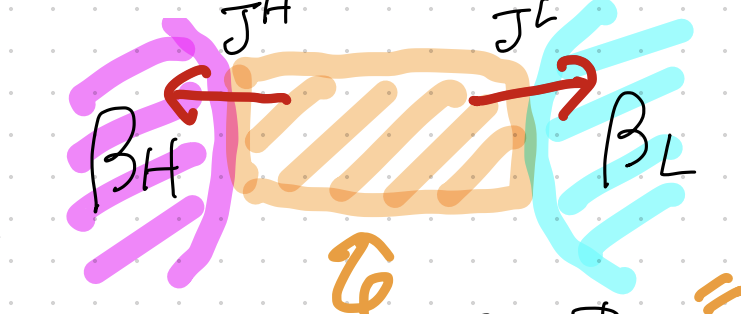
\includegraphics[width=100mm]{set.png}
    \end{center}
    \caption{設定}
    \label{fig:set}
\end{figure}

系が二つの熱浴に接触しているとする。$\alpha = \text{H,L}$で、それぞれの熱浴の逆温度を$\beta_{\alpha}$、遷移レートを$\omega_{j \to k}(t)$、系のエネルギーを$E_j(t)$とする。このとき、局所詳細釣り合い条件は、
\begin{align}
  \log \frac{\omega_{j \to k}(t)}{\omega_{k \to j}(t)} = \beta_{\alpha(j,k)}(E_j(t) - E_k(t))
\end{align}
である。($\alpha(j,k) = \text{H,L}$)\\
熱浴への熱の流れは、
\begin{align}
  {J}^{\alpha}_{j\to k}(t) =
  \begin{cases}
    E_j(t) - E_k(t) & \alpha(j,k) = \alpha\\
    0 & \text{otherwise}
    \end{cases}
\end{align}
である。また、エントロピー生成は、
\begin{align}
  \theta_{j \to k}(t) & \beta_{\alpha(j,k)}(E_j(t) - E_k(t))\\
    &= \beta_{\text{H}}J^{\text{H}}_{j\to k}(t) + \beta_{\text{L}}J^{\text{L}}_{j\to k}(t)
\end{align}
である。\\
\textbf{仮定}\\
\begin{figure}[H]
    \begin{center}
    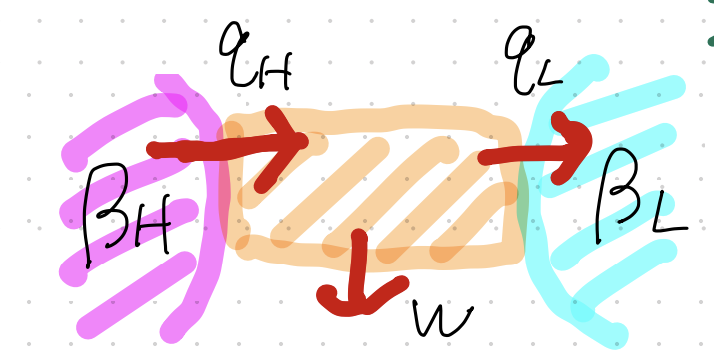
\includegraphics[width=100mm]{set2.png}
    \end{center}
    \caption{仮定}
    \label{fig:set2}
\end{figure}

以下の極限が存在し、その極限値が正であるとする:
\begin{align}
  q_H &= -\lim_{\tau \to \infty}\frac{1}{\tau}\int_0^{\tau} \dd{t}\ev{\hat{J}^H(t)}_t>0\\
  q_L &= \lim_{\tau \to \infty}\frac{1}{\tau}\int_0^{\tau} \dd{t}\ev{\hat{J}^L(t)}_t>0
\end{align}
これは、高温熱浴から系に入ってくる熱流および、低温熱浴に流れる熱流の時間平均である。また、このとき、平均のパワー(仕事率)は、
\begin{align}
  W = q_H - q_L
\end{align}
であり、効率は、
\begin{align}
  \eta = \frac{W}{q_H} = 1 - \frac{q_L}{q_H}
\end{align}
である。このとき、以下の不等式が成立する。

\begin{itembox}[l]{\textbf{Thm:熱機関の、パワーと効率のトレードオフ}}
    熱機関のパワーと効率は、以下の不等式を満たす:
    \begin{align}
      (q_H + q_L)^2 \leq \overline{\Xi} \beta_L q_H (\eta_{\text{C}} - \eta) 
    \end{align}

\end{itembox}
\textbf{Prf}\\
今、
\begin{align}
    \lim_{\tau \to \infty}\frac{1}{\tau}\int_0^{\tau} \dd{t}\ev{\hat{\theta}_t}_t &= -\beta_H q_H + \beta_L q_L\\
    &= -\beta_H q_H + \beta_L (q_H - W)\\
    &= \beta_L q_H \qty(-\frac{\beta_H}{\beta_L} + 1 - \frac{W}{q_H})\\
      &= \beta_L q_H (\eta_{\text{C}} - \eta) (\geq 0)
  \end{align}
  である。また、
\begin{align}
  g_{j \to k}(t) = \hat{J}_{j \to k}^L(t) - \hat{J}_{j \to k}^H(t)
\end{align}
とする。このとき、Shiraishi-Saito不等式より、
\begin{align}
  \left(\frac{1}{\tau}\int_0^{\tau} \dd{t}\ev{\hat{g}(t)}_t\right)^2 \leq \overline{\Xi} \lim_{\tau \to \infty}\frac{1}{\tau}\int_0^{\tau} \dd{t}\ev{\hat{\theta}_t}_t
\end{align}
である。ここで、
\begin{align}
  \overline{\Xi} = \lim_{\tau \to \infty}\frac{1}{\tau} \dd{t} \frac{1}{2}\sum_{j,k(j \neq k)}^{\Omega} R_{kj}(t)p_j(t) (E_j(t) - E_k(t))^2
\end{align}
である。(これは、どれくらいactiveに熱のやり取りをするかを表している。)このとき、
\begin{align}
  \qty(\frac{1}{\tau}\int_0^{\tau} \dd{t}\ev{\hat{g}(t)}_t)^2 = (q_H + q_L)^2
\end{align}
である。よって、
\begin{align}
  (q_H + q_L)^2 \leq \overline{\Xi} \beta_L q_H (\eta_{\text{C}} - \eta)
\end{align}
である。よって示された。\qedsymbol\\

上で得られた不等式を変形すると、
\begin{align}
  \overline{\Xi} \beta_L(\eta_{\text{C}} - \eta) \geq \frac{(q_H + q_L)^2}{q_H} \geq q_H + q_L
\end{align}
となる。これは、効率がカルノーサイクルに近づくと、$q_H, q_L$が0に近づくことを表している。このもとで、パワーは0に近づくことがわかる。\\
あるいは、以下のようにも変形できる:
\begin{align}
  W &\leq \overline{\Xi} \beta_L\frac{q_H}{(q_H + q_L)^2}(\eta_{\text{C}} - \eta)W\\
  &= \overline{\Xi} \beta_L\frac{q_H}{(q_H + q_L)^2}\eta(\eta_{\text{C}} - \eta)\quad (\because W = q_H \eta)\\
    &\leq \overline{\Xi} \beta_L\eta(\eta_{\text{C}} - \eta)
\end{align}
これは、効率がカルノーサイクルに近づくと、パワーが0に近づくことを直接的に示している。\\

\subsubsection{熱力学的不確定性関係}

\section{量子力学}

\section{相対論}

\section{場の量子論}

\section{その他}





\end{document}